\chapter{Additional Material for Chapter 3}
\graphicspath{{figures/ch_3/}}
\addtocontents{toc}{\protect\setcounter{tocdepth}{0}}
\section{Monotonicity of \texorpdfstring{\( \MakeLowercase{g} \)}{g}}
\label{ch_3:sec:monotonicity}
It is clear that \( g \) is monotonic within each of its piecewise-defined functions.
In the following sections, we consider if monotonicity holds at the change points between piecewise functions.

\subsection{Monotonicity in \texorpdfstring{\( \hat{\phi}_p \)}{ϕp}}


\begin{itemize}
	\item Case 1: \( \hat{\phi}_n < \hat{\theta}_1 \). Not monotonic. \\
\begin{equation}
g(\hat{\theta}_1, \hat{\phi}_n, \hat{\phi}_p)
=
\left\{
\begin{array}{ll}
0 & \hat{\phi}_p < \hat{\phi}_n < \hat{\theta}_1  \\
0 & \hat{\phi}_n = \hat{\phi}_p < \hat{\theta}_1 \\
1 &	\hat{\phi}_n < \hat{\phi}_p < \hat{\theta}_1 \\
\frac{\hat{\theta}_1 - \hat{\phi}_n}{\hat{\phi}_p - \hat{\phi}_n} = 1 & \hat{\phi}_n < \hat{\phi}_p = \hat{\theta}_1 \\
\frac{\hat{\theta}_1 - \hat{\phi}_n}{\hat{\phi}_p - \hat{\phi}_n} & \hat{\phi}_n < \hat{\theta}_1 < \hat{\phi}_p \\
\end{array}
\right.
\end{equation}

\item Case 2: \( \hat{\theta}_1 < \hat{\phi}_n \). Monotonic. \\
\begin{equation}
g(\hat{\theta}_1, \hat{\phi}_n, \hat{\phi}_p)
=
\left\{
\begin{array}{ll}
0 \hspace*{3em} & \hat{\phi}_p < \hat{\theta}_1 < \hat{\phi}_n  \\
0 & \hat{\theta}_1 = \hat{\phi}_p < \hat{\phi}_n \\
0 &	\hat{\theta}_1 < \hat{\phi}_p < \hat{\phi}_n \\
0 & \hat{\theta}_1 < \hat{\phi}_p = \hat{\phi}_n \\
0 & \hat{\theta}_1 < \hat{\phi}_n < \hat{\phi}_p \\
\end{array}
\right.
\end{equation}

\item Case 3: \( \hat{\theta}_1 = \hat{\phi}_n \). Monotonic. \\
\begin{equation}
g(\hat{\theta}_1, \hat{\phi}_n, \hat{\phi}_p)
=
\left\{
\begin{array}{ll}
0 & \hat{\phi}_p < \hat{\theta}_1 = \hat{\phi}_n	\\
\frac{\hat{\theta}_1 - \hat{\phi}_n}{\hat{\phi}_p - \hat{\phi}_n} = \frac{0}{0} \equiv 0 & \hat{\phi}_p = \hat{\theta}_1 = \hat{\phi}_n 	\\
\frac{\hat{\theta}_1 - \hat{\phi}_n}{\hat{\phi}_p - \hat{\phi}_n} = \frac{0}{\hat{\phi}_p - \hat{\phi}_n} = 0 & \hat{\theta}_1 = \hat{\phi}_n < \hat{\phi}_p	\\
\end{array}
\right.
\end{equation}
\end{itemize}

\subsection{Monotonicity in \texorpdfstring{\( \hat{\theta}_1 \)}{θ1}}


\begin{itemize}
	\item Case 1: \( \hat{\phi}_n < \hat{\phi}_p \). Monotonic. \\
\begin{equation}
g(\hat{\theta}_1, \hat{\phi}_n, \hat{\phi}_p)
=
\left\{
\begin{array}{ll}
0 & \hat{\theta}_1 < \hat{\phi}_n < \hat{\phi}_p  \\
\frac{\hat{\theta}_1 - \hat{\phi}_n}{\hat{\phi}_p - \hat{\phi}_n} = 0 & \hat{\phi}_n = \hat{\theta}_1 < \hat{\phi}_p \\
\frac{\hat{\theta}_1 - \hat{\phi}_n}{\hat{\phi}_p - \hat{\phi}_n} &	\hat{\phi}_n < \hat{\theta}_1 < \hat{\phi}_p \\
\frac{\hat{\theta}_1 - \hat{\phi}_n}{\hat{\phi}_p - \hat{\phi}_n} = 1 & \hat{\phi}_n < \hat{\theta}_1 = \hat{\phi}_p \\
1 & \hat{\phi}_n < \hat{\phi}_p < \hat{\theta}_1 \\
\end{array}
\right.
\end{equation}

\item Case 2: \( \hat{\phi}_p < \hat{\phi}_n \). Monotonic. \\
\begin{equation}
g(\hat{\theta}_1, \hat{\phi}_n, \hat{\phi}_p)
=
\left\{
\begin{array}{ll}
0 \hspace*{3em} & \hat{\theta}_1 < \hat{\phi}_p < \hat{\phi}_n  \\
0 & \hat{\phi}_p = \hat{\theta}_1 < \hat{\phi}_n \\
0 &	\hat{\phi}_p < \hat{\theta}_1 < \hat{\phi}_n \\
0 & \hat{\phi}_p < \hat{\theta}_1 = \hat{\phi}_n \\
0 & \hat{\phi}_p < \hat{\phi}_n < \hat{\theta}_1 \\
\end{array}
\right.
\end{equation}

\item Case 3: \( \hat{\phi}_p = \hat{\phi}_n \). Monotonic. \\
\begin{equation}
g(\hat{\theta}_1, \hat{\phi}_n, \hat{\phi}_p)
=
\left\{
\begin{array}{ll}
0 & \hat{\theta}_1 < \hat{\phi}_p = \hat{\phi}_n	\\
\frac{\hat{\theta}_1 - \hat{\phi}_n}{\hat{\phi}_p - \hat{\phi}_n} = \frac{0}{0} \equiv 0 & \hat{\theta}_1 = \hat{\phi}_p = \hat{\phi}_n 	\\
0 & \hat{\phi}_p = \hat{\phi}_n < \hat{\theta}_1	\\
\end{array}
\right.
\end{equation}
\end{itemize}

\subsection{Monotonicity in \texorpdfstring{\( \hat{\phi}_n \)}{ϕ n}}


\begin{itemize}
	\item Case 1: \( \hat{\phi}_p < \hat{\theta}_1 \). Monotonic. \\
\begin{equation}
g(\hat{\theta}_1, \hat{\phi}_n, \hat{\phi}_p)
=
\left\{
\begin{array}{ll}
1 \hspace*{3em} & \hat{\phi}_n < \hat{\phi}_p < \hat{\theta}_1  \\
0 & \hat{\phi}_p = \hat{\phi}_n < \hat{\theta}_1 \\
0 &	\hat{\phi}_p < \hat{\phi}_n < \hat{\theta}_1 \\
0 & \hat{\phi}_p < \hat{\phi}_n = \hat{\theta}_1 \\
0 & \hat{\phi}_p < \hat{\theta}_1 < \hat{\phi}_n \\
\end{array}
\right.
\end{equation}

\item Case 2: \( \hat{\theta}_1 < \hat{\phi}_p \). Monotonic.
\begin{equation}
g(\hat{\theta}_1, \hat{\phi}_n, \hat{\phi}_p)
=
\left\{
\begin{array}{ll}
\frac{\hat{\theta}_1 - \hat{\phi}_n}{\hat{\phi}_p - \hat{\phi}_n} & \hat{\phi}_n < \hat{\theta}_1 < \hat{\phi}_p  \\
\frac{\hat{\theta}_1 - \hat{\phi}_n}{\hat{\phi}_p - \hat{\phi}_n} = \frac{0}{\hat{\phi}_p - \hat{\phi}_n} = 0 & \hat{\theta}_1 = \hat{\phi}_n < \hat{\phi}_p \\
0 &	\hat{\theta}_1 < \hat{\phi}_n < \hat{\phi}_p \\
0 & \hat{\theta}_1 < \hat{\phi}_n = \hat{\phi}_p \\
0 & \hat{\theta}_1 < \hat{\phi}_p < \hat{\phi}_n \\
\end{array}
\right.
\end{equation}

\item Case 3: \( \hat{\theta}_1 = \hat{\phi}_p \). Monotonic. \\
\begin{equation}
g(\hat{\theta}_1, \hat{\phi}_n, \hat{\phi}_p)
=
\left\{
\begin{array}{ll}
\frac{\hat{\theta}_1 - \hat{\phi}_n}{\hat{\phi}_p - \hat{\phi}_n} = 1 & \hat{\phi}_n < \hat{\theta}_1 = \hat{\phi}_p	\\
\frac{\hat{\theta}_1 - \hat{\phi}_n}{\hat{\phi}_p - \hat{\phi}_n} = \frac{0}{0} \equiv 0 & \hat{\phi}_n = \hat{\theta}_1 = \hat{\phi}_p 	\\
0 & \hat{\theta}_1 = \hat{\phi}_p < \hat{\phi}_n	\\
\end{array}
\right.
\end{equation}
\end{itemize}

\section{Additional Figures}

\begin{figure}
\centering
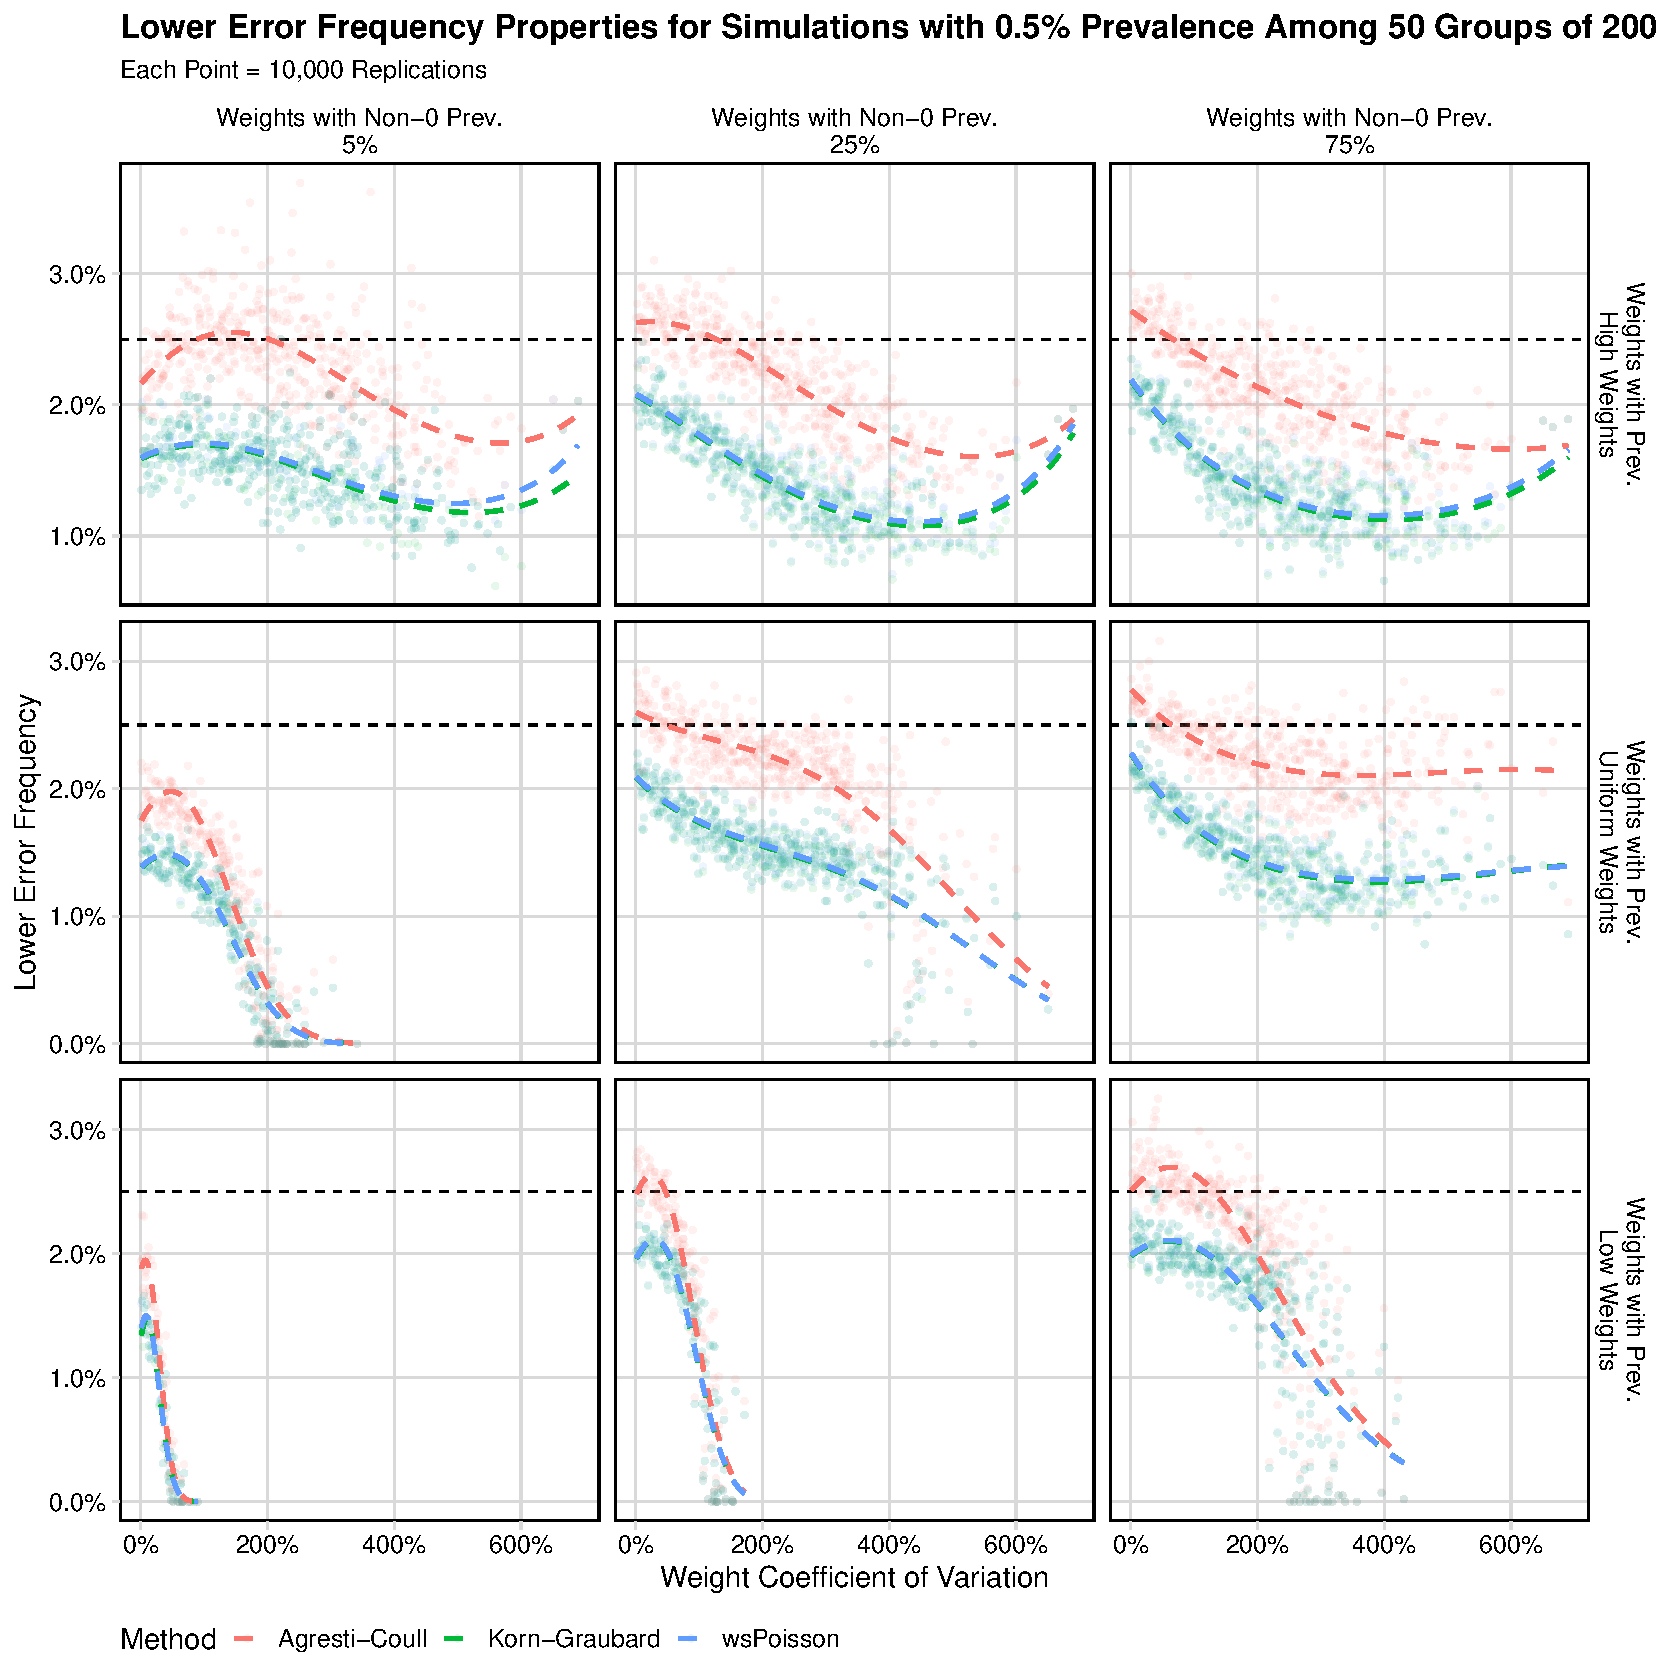
\includegraphics[width=0.8\textwidth]{perfect_lower_error_frequency_50_groups_0_005_prev}
\caption{Lower error properties for the wsPoisson model and two standard methods, the Dean-Pagano modification of the Agresti-Coull method and of the Korn-Graubard method.
Each point represents 10,000 simulations of datasets from a population with 0.5\% prevalence, where 50 groups of 200 people are sampled.
The horizontal dashed line indicates the nominal lower error rate, 2.5\%.
Colored dashed lines are estimates from a logistic regression model using quadratic splines.}
\label{ch_3:fig:perfect_lower_error_frequency_50_groups_0_005_prev}
\end{figure}

\begin{figure}
\centering
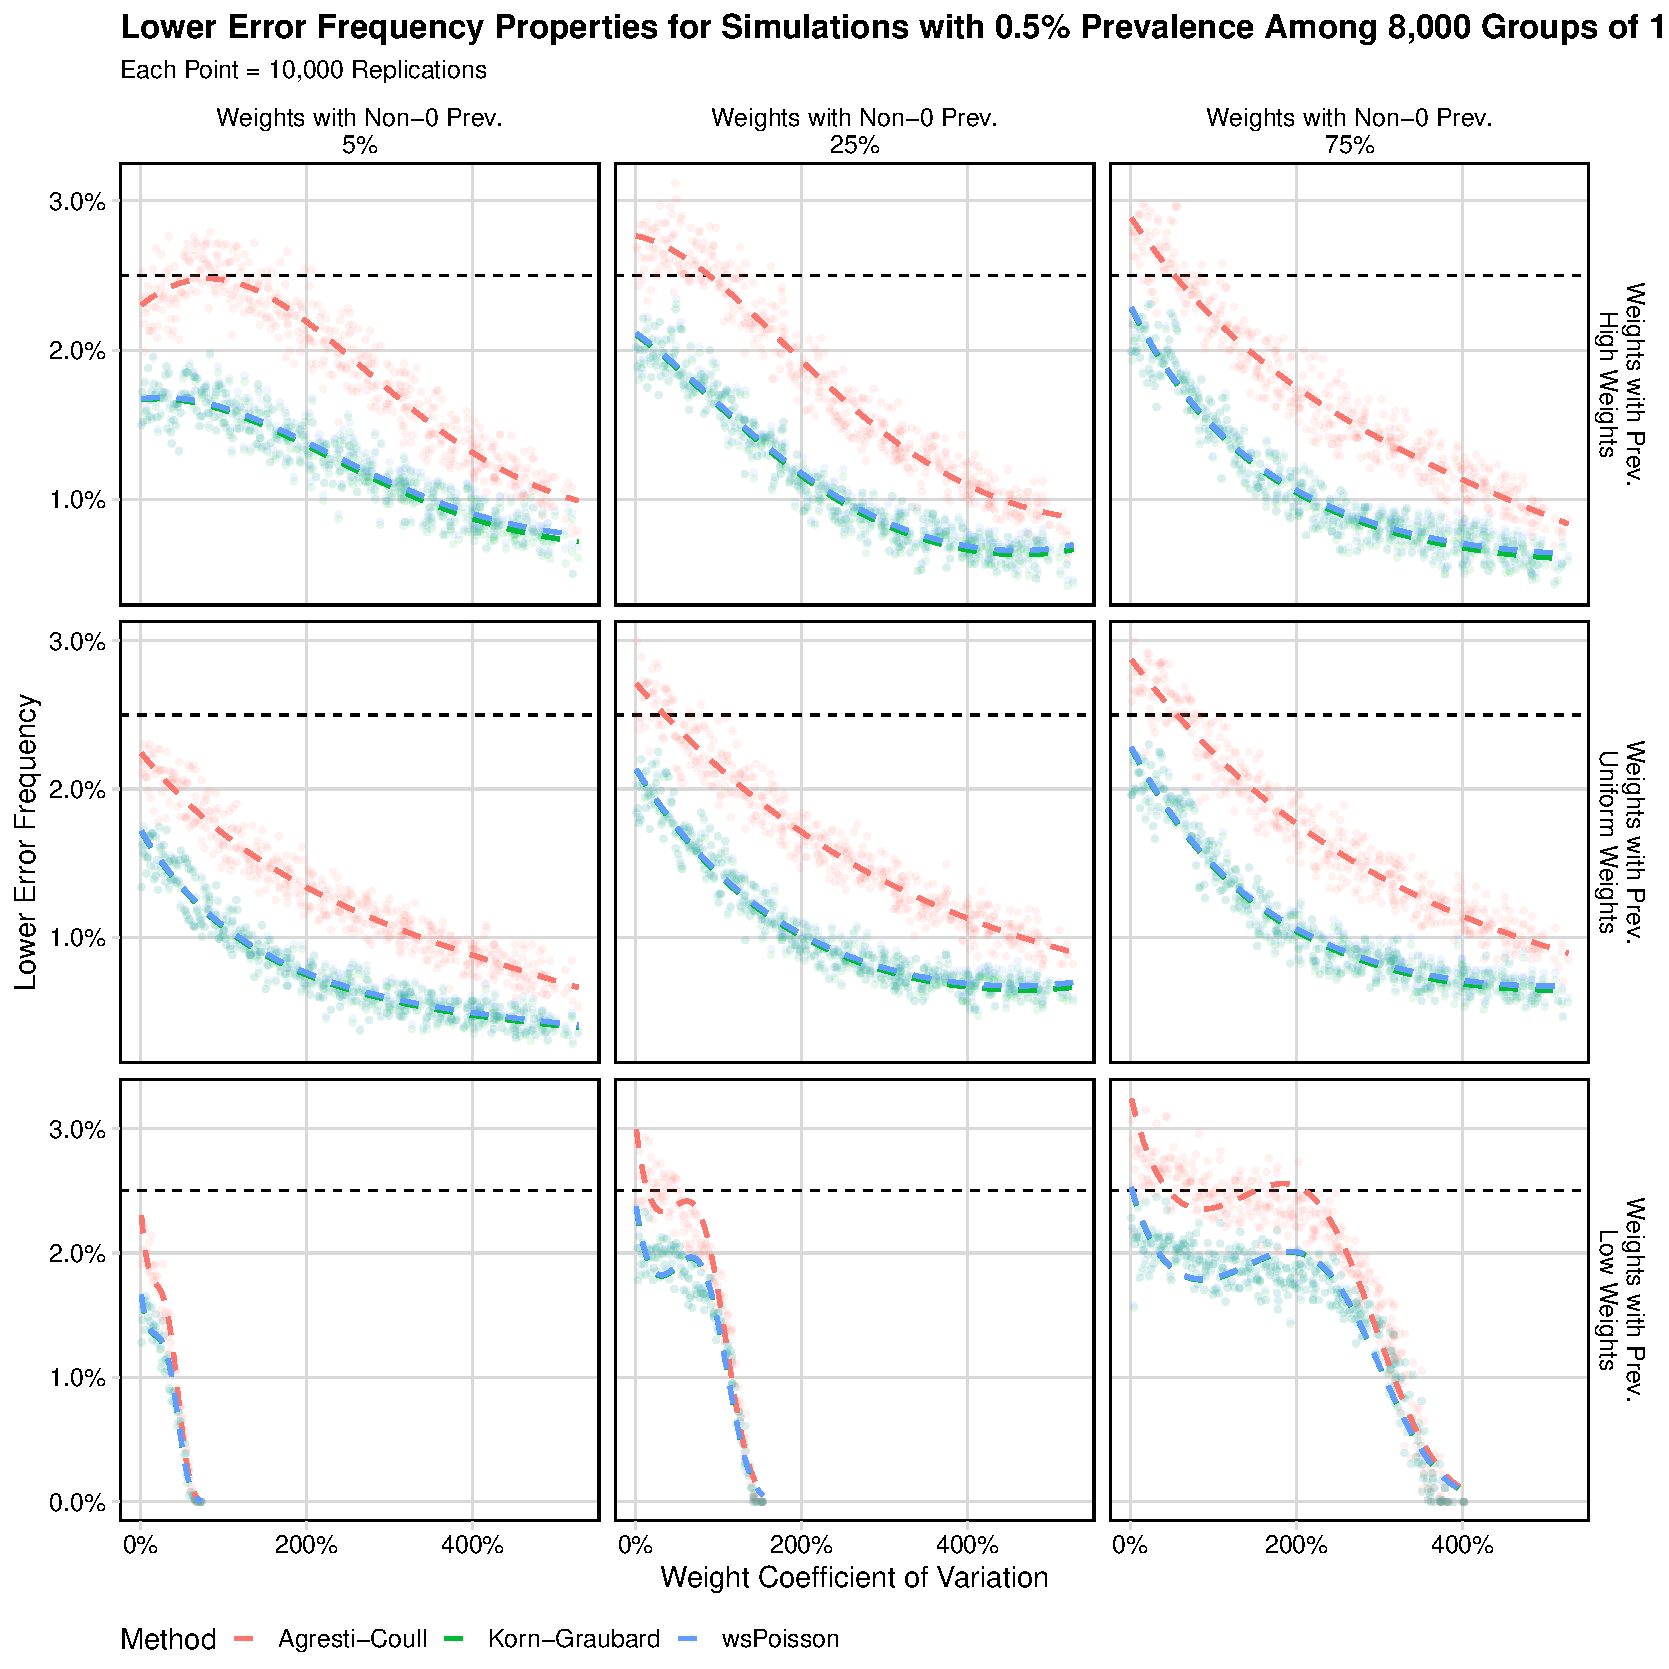
\includegraphics[width=0.8\textwidth]{perfect_lower_error_frequency_8000_groups_0_005_prev}
\caption{Lower error properties for the wsPoisson model and two standard methods, the Dean-Pagano modification of the Agresti-Coull method and of the Korn-Graubard method.
Each point represents 10,000 simulations of datasets from a population with 0.5\% prevalence, where 8000 individuals are sampled.
The horizontal dashed line indicates the nominal lower error rate, 2.5\%.
Colored dashed lines are estimates from a logistic regression model using quadratic splines.}
\label{ch_3:fig:perfect_lower_error_frequency_8000_groups_0_005_prev}
\end{figure}

\begin{figure}
\centering
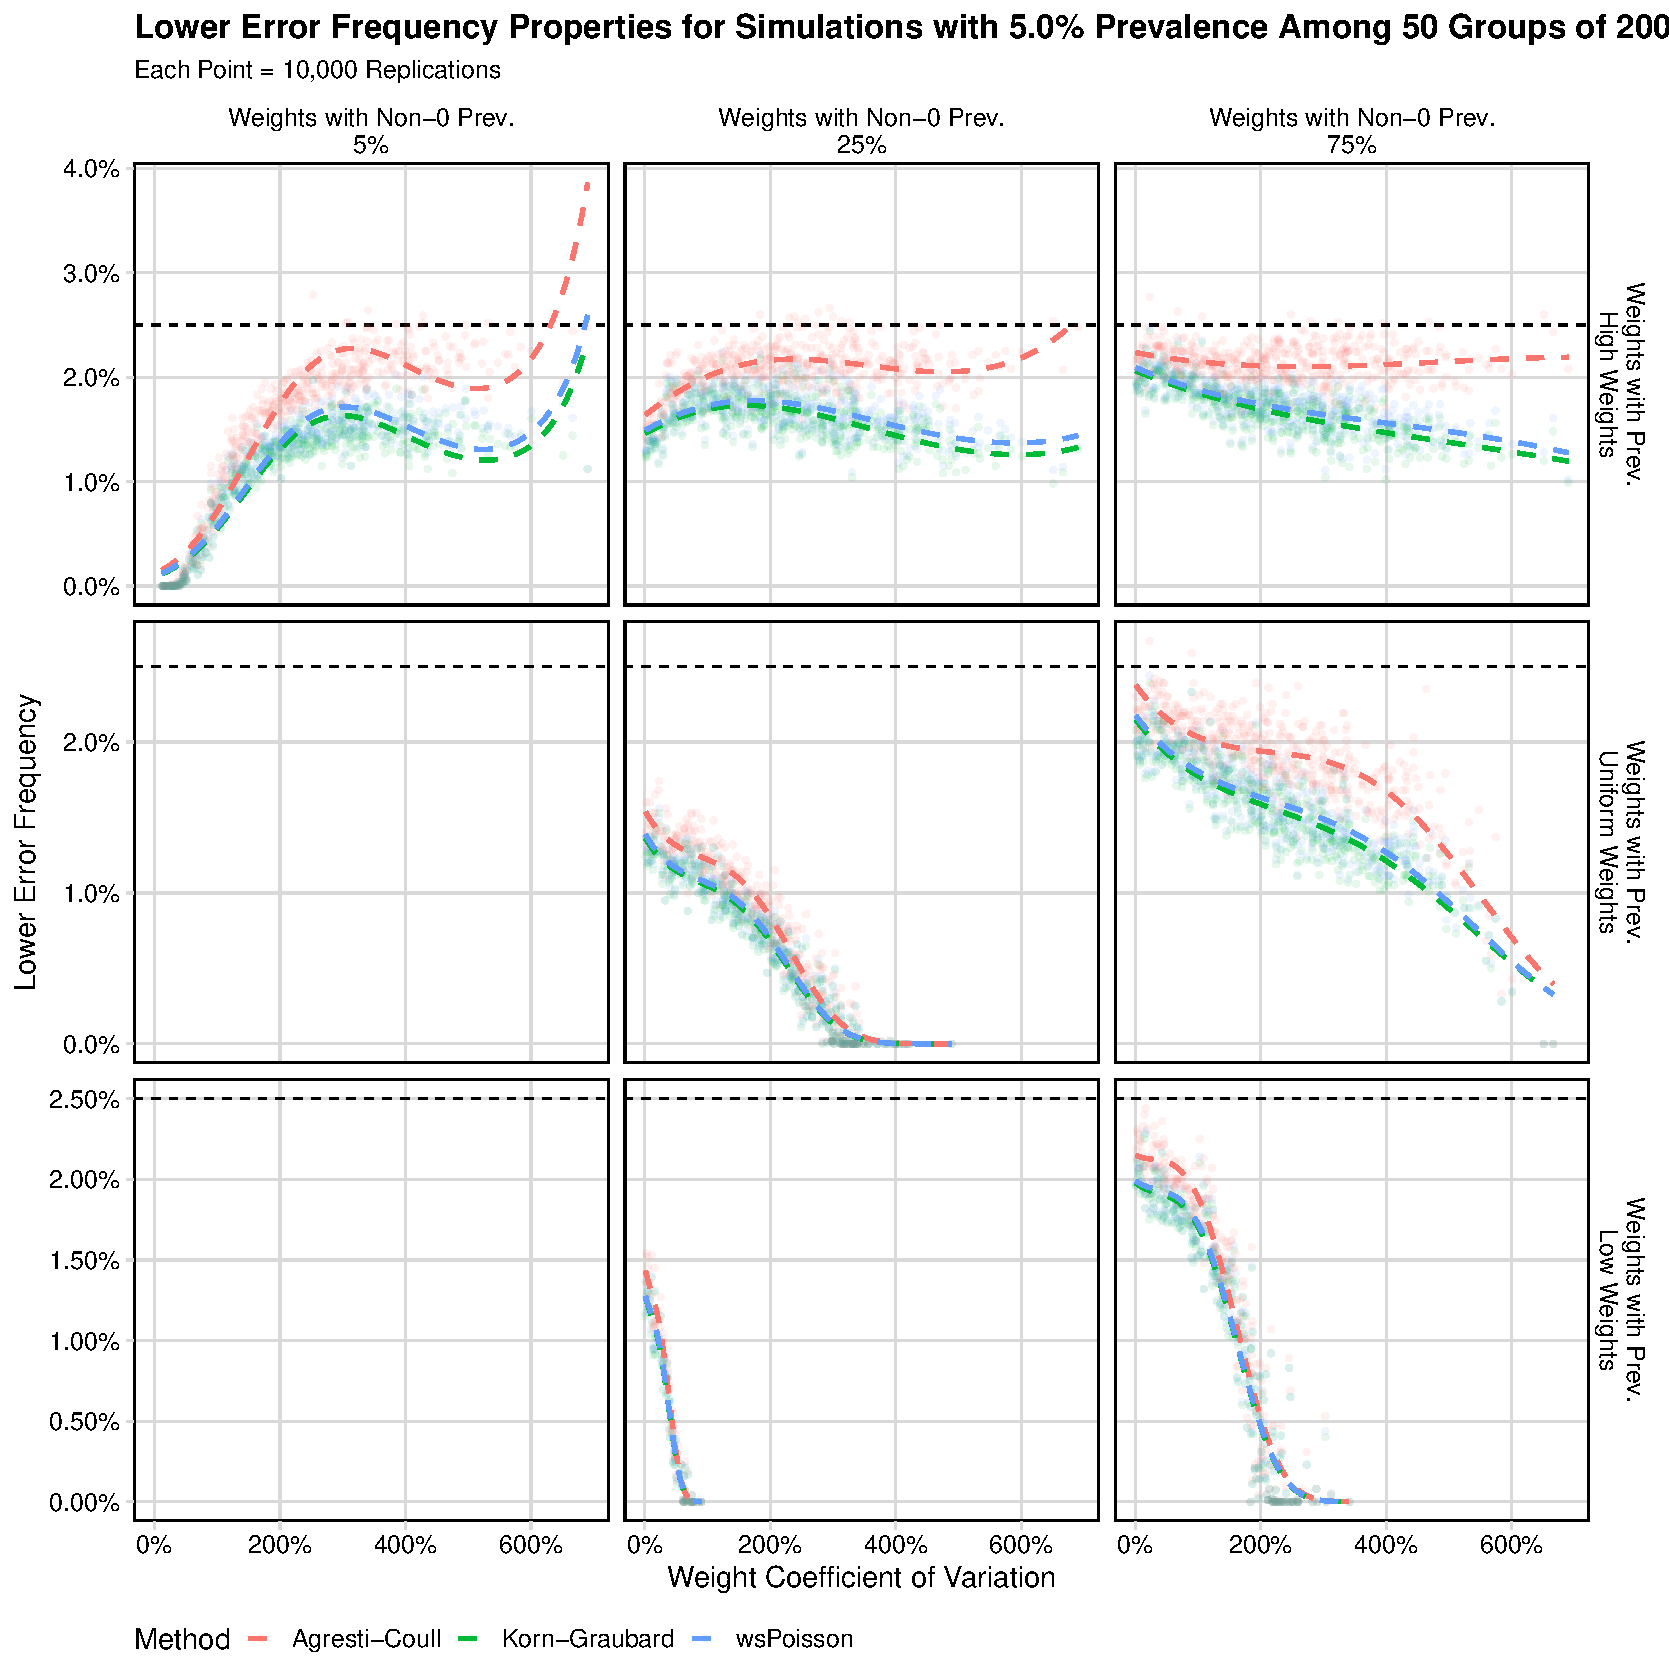
\includegraphics[width=0.8\textwidth]{perfect_lower_error_frequency_50_groups_0_05_prev}
\caption{Lower error properties for the wsPoisson model and two standard methods, the Dean-Pagano modification of the Agresti-Coull method and of the Korn-Graubard method.
Each point represents 10,000 simulations of datasets from a population with 5\% prevalence, where 50 groups of 200 people are sampled.
The horizontal dashed line indicates the nominal lower error rate, 2.5\%.
Colored dashed lines are estimates from a logistic regression model using quadratic splines.}
\label{ch_3:fig:perfect_lower_error_frequency_50_groups_0_05_prev}
\end{figure}

\begin{figure}
\centering
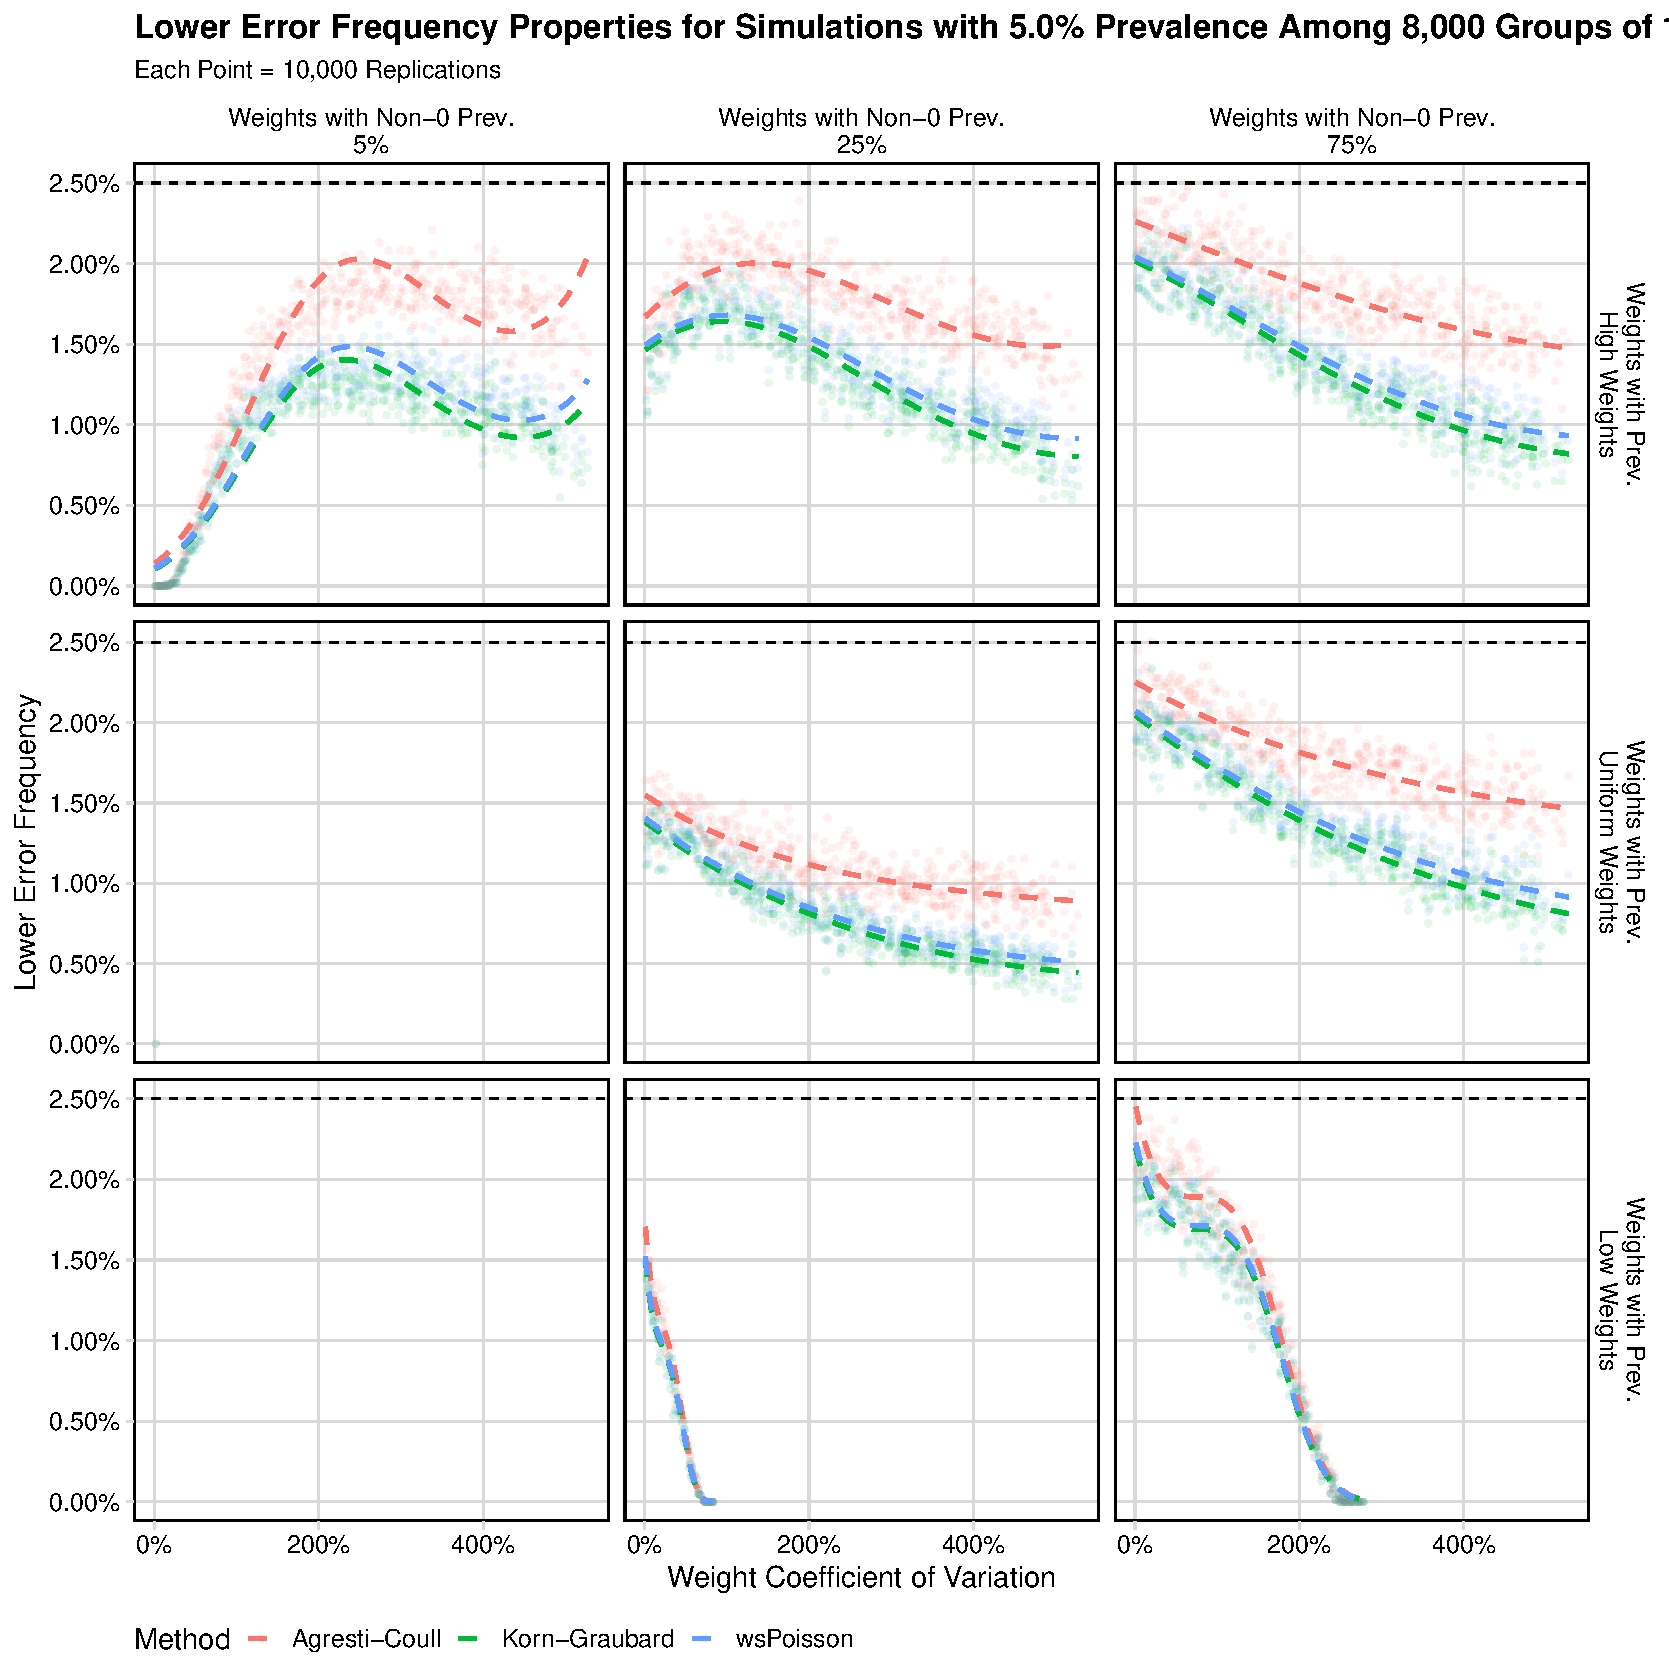
\includegraphics[width=0.8\textwidth]{perfect_lower_error_frequency_8000_groups_0_05_prev}
\caption{Lower error properties for the wsPoisson model and two standard methods, the Dean-Pagano modification of the Agresti-Coull method and of the Korn-Graubard method.
Each point represents 10,000 simulations of datasets from a population with 5\% prevalence, where 8000 individuals are sampled.
The horizontal dashed line indicates the nominal lower error rate, 2.5\%.
Colored dashed lines are estimates from a logistic regression model using quadratic splines.}
\label{ch_3:fig:perfect_lower_error_frequency_8000_groups_0_05_prev}
\end{figure}

\begin{figure}
\centering
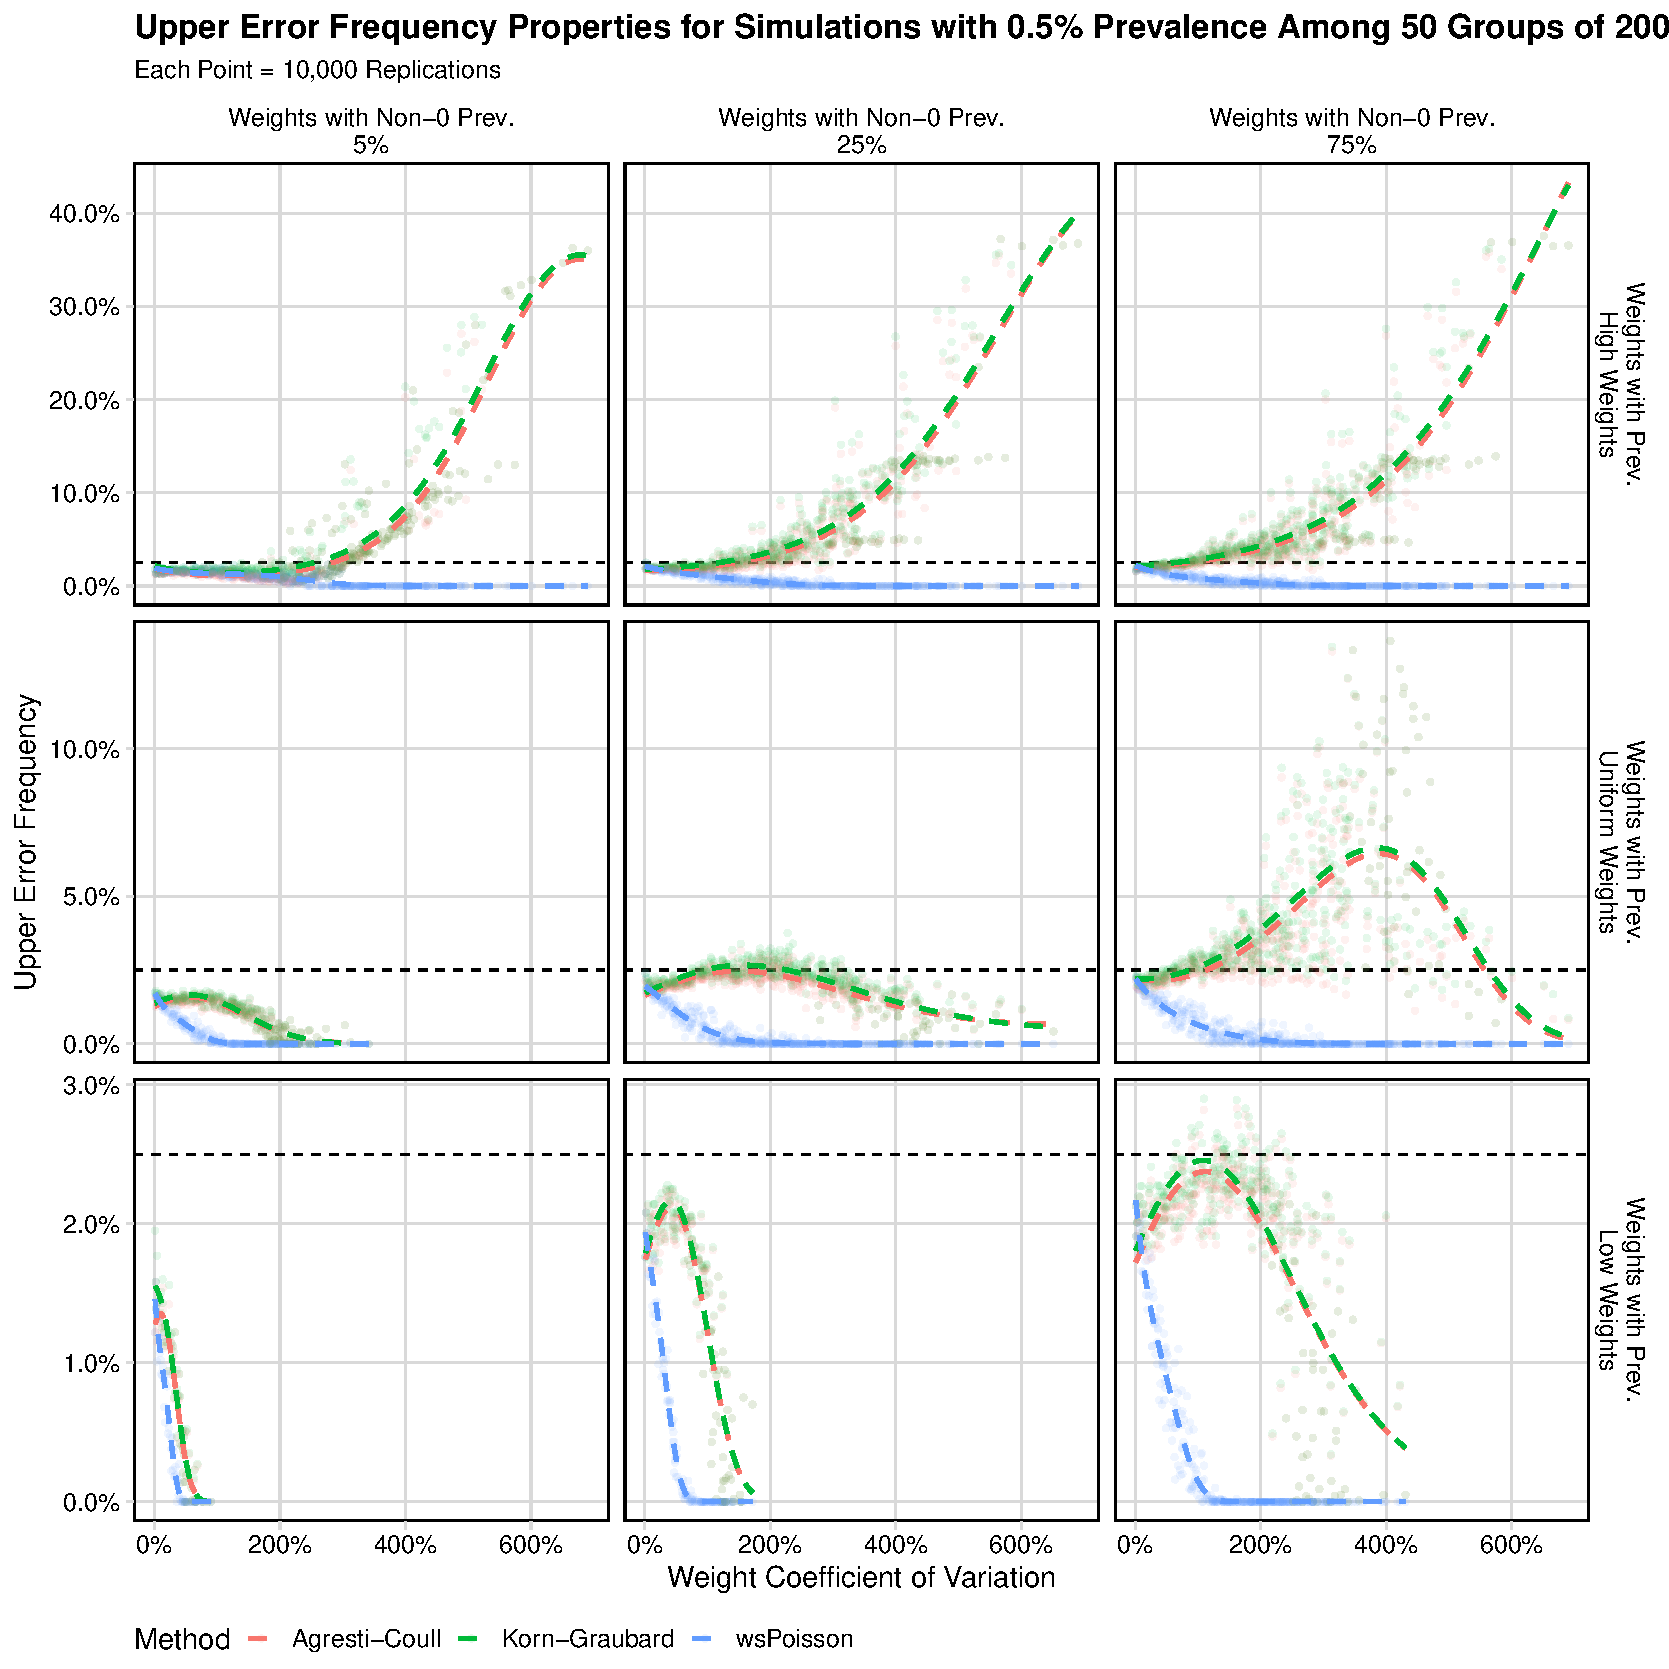
\includegraphics[width=0.8\textwidth]{perfect_upper_error_frequency_50_groups_0_005_prev}
\caption{Upper error properties for the wsPoisson model and two standard methods, the Dean-Pagano modification of the Agresti-Coull method and of the Korn-Graubard method.
Each point represents 10,000 simulations of datasets from a population with 0.5\% prevalence, where 50 groups of 200 people are sampled.
The horizontal dashed line indicates the nominal upper error rate, 2.5\%.
Colored dashed lines are estimates from a logistic regression model using quadratic splines.}
\label{ch_3:fig:perfect_upper_error_frequency_50_groups_0_005_prev}
\end{figure}

\begin{figure}
\centering
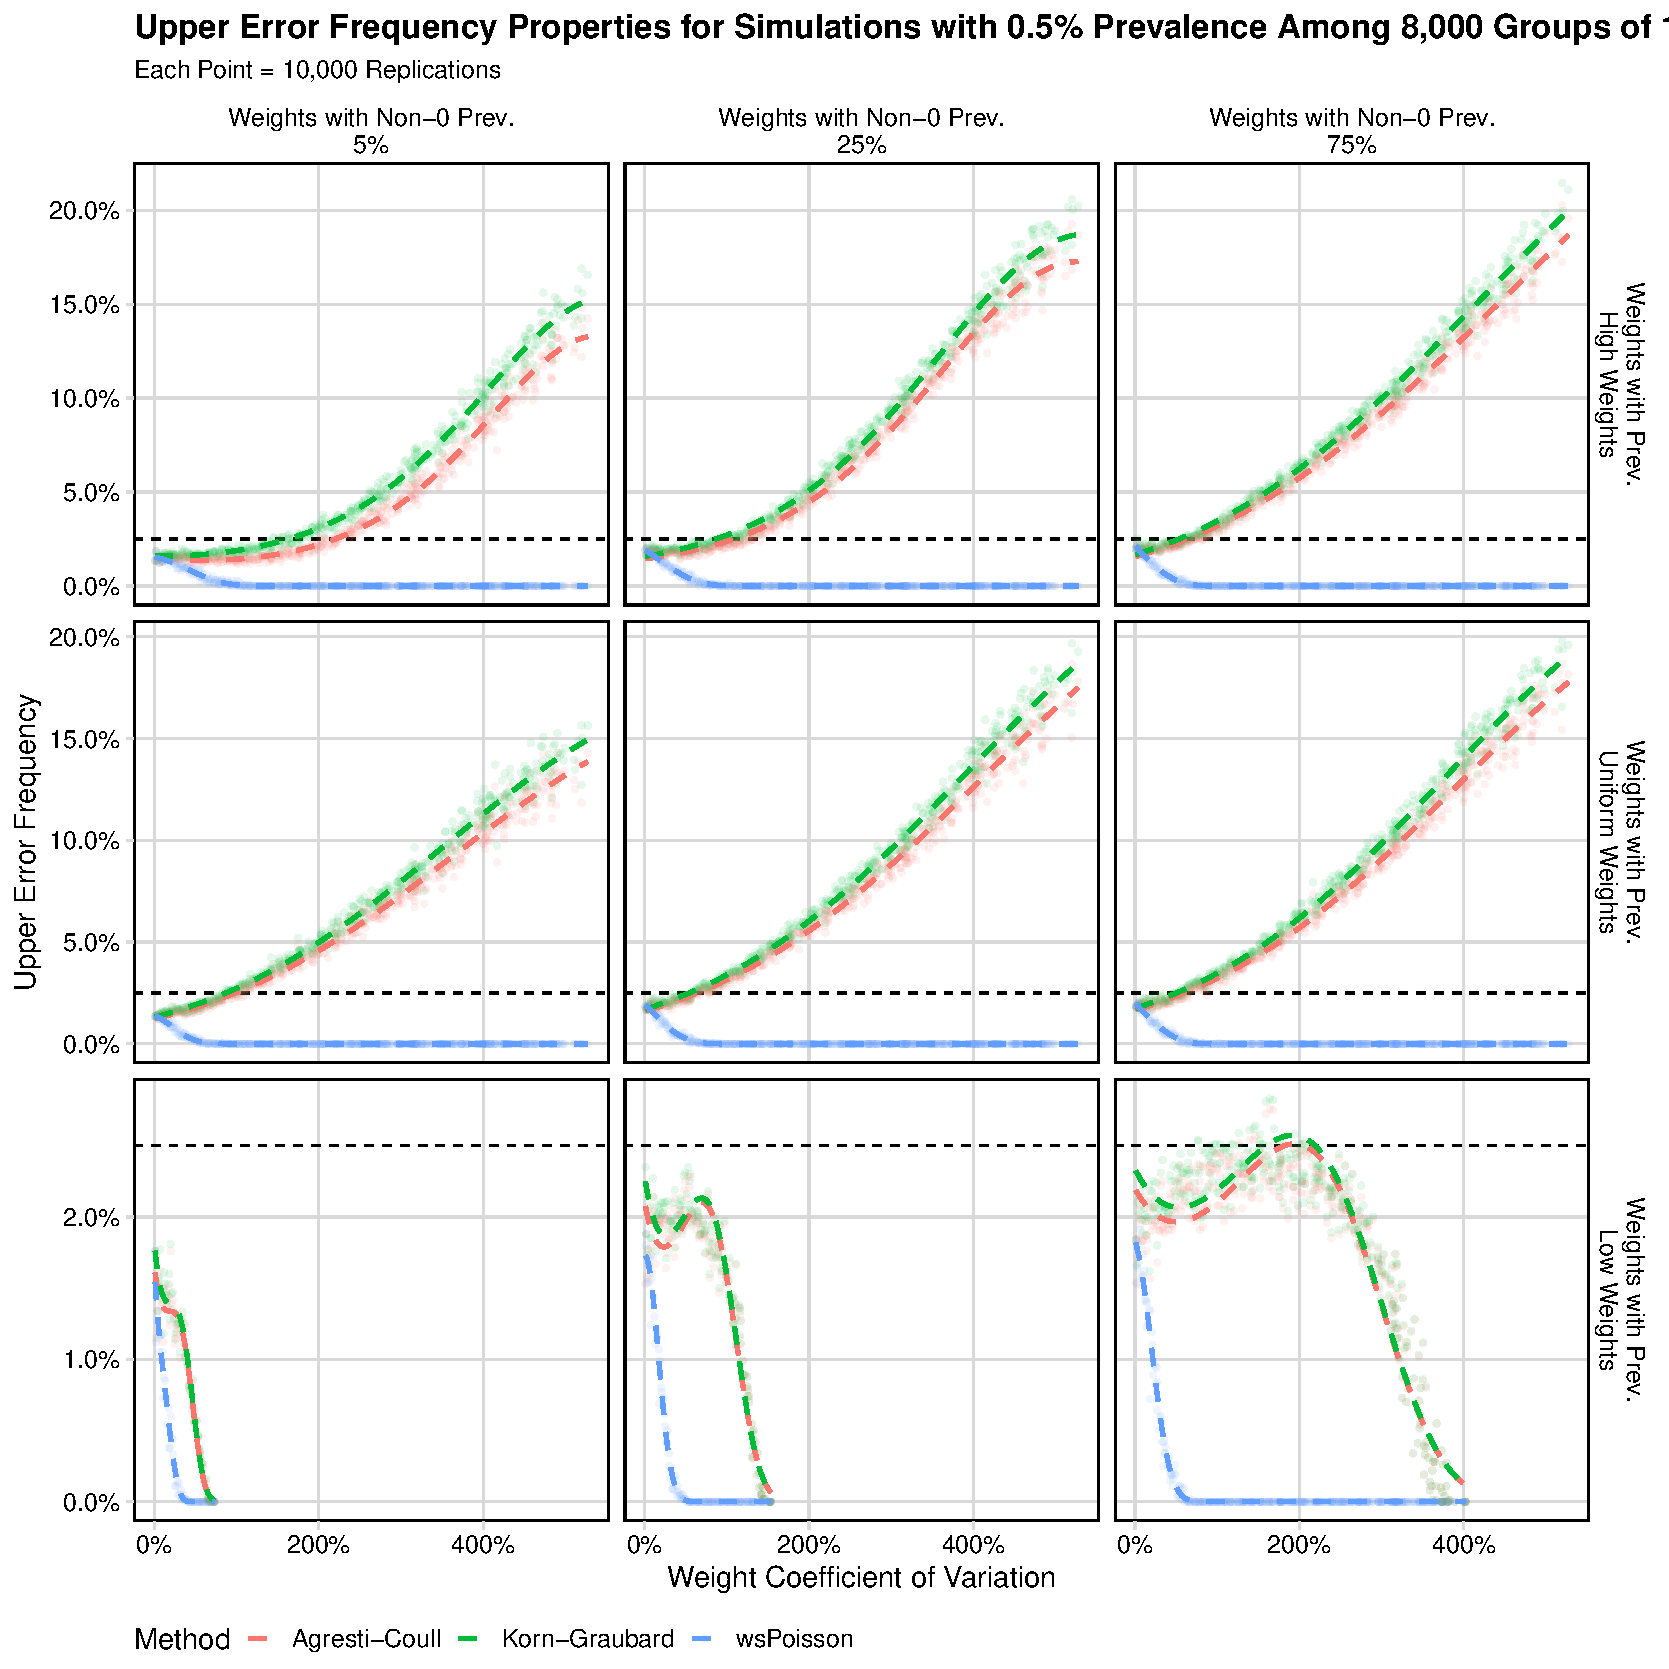
\includegraphics[width=0.8\textwidth]{perfect_upper_error_frequency_8000_groups_0_005_prev}
\caption{Upper error properties for the wsPoisson model and two standard methods, the Dean-Pagano modification of the Agresti-Coull method and of the Korn-Graubard method.
Each point represents 10,000 simulations of datasets from a population with 0.5\% prevalence, where 8000 individuals are sampled.
The horizontal dashed line indicates the nominal upper error rate, 2.5\%.
Colored dashed lines are estimates from a logistic regression model using quadratic splines.}
\label{ch_3:fig:perfect_upper_error_frequency_8000_groups_0_005_prev}
\end{figure}

\begin{figure}
\centering
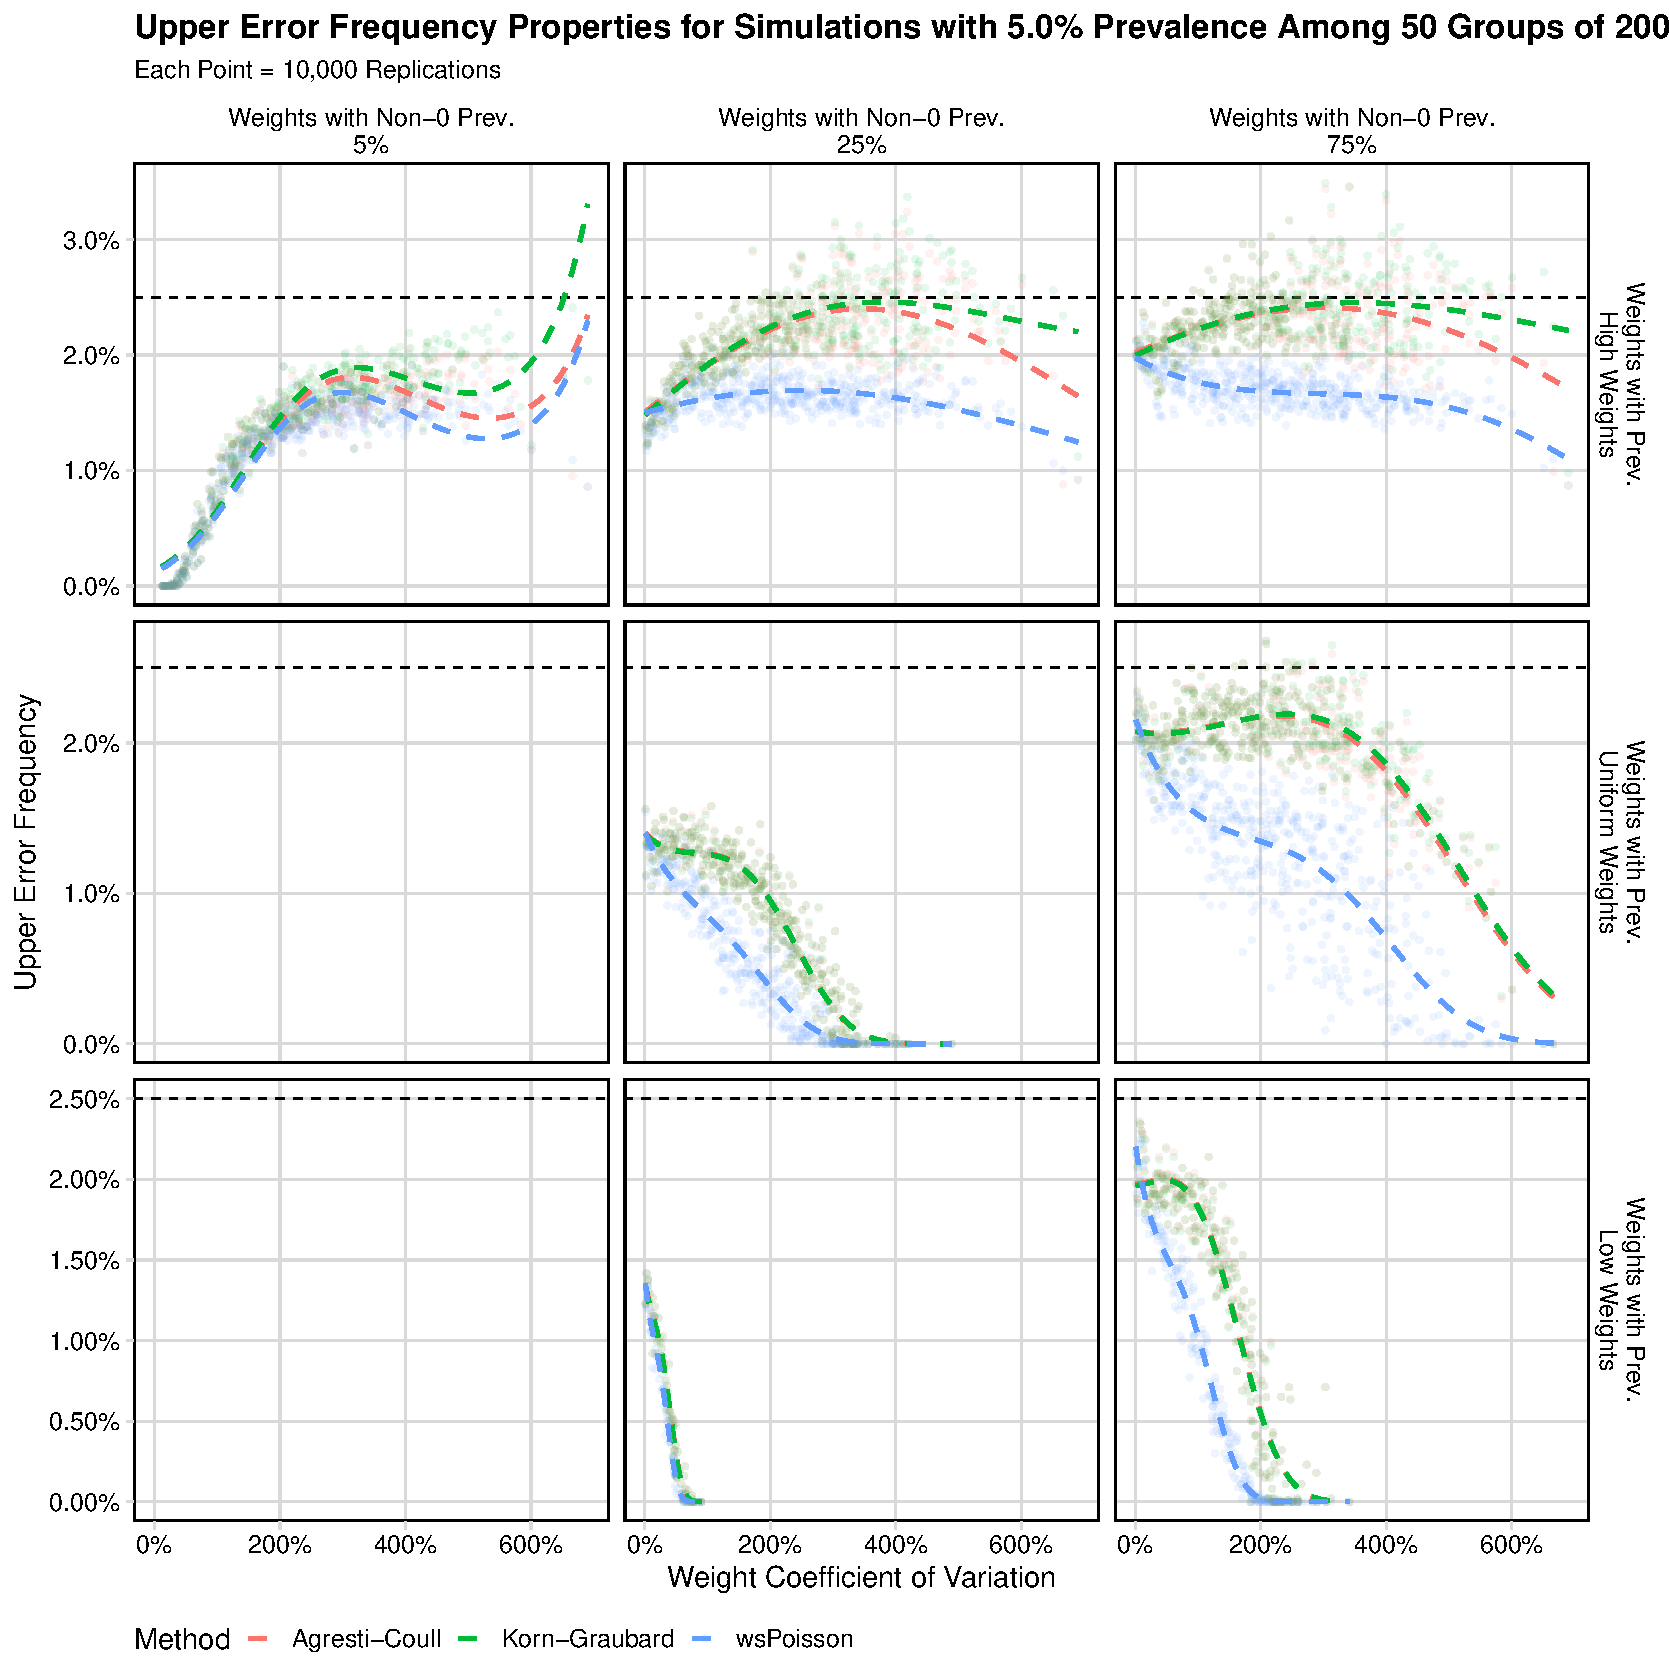
\includegraphics[width=0.8\textwidth]{perfect_upper_error_frequency_50_groups_0_05_prev}
\caption{Upper error properties for the wsPoisson model and two standard methods, the Dean-Pagano modification of the Agresti-Coull method and of the Korn-Graubard method.
Each point represents 10,000 simulations of datasets from a population with 5\% prevalence, where 50 groups of 200 people are sampled.
The horizontal dashed line indicates the nominal upper error rate, 2.5\%.
Colored dashed lines are estimates from a logistic regression model using quadratic splines.}
\label{ch_3:fig:perfect_upper_error_frequency_50_groups_0_05_prev}
\end{figure}

\begin{figure}
\centering
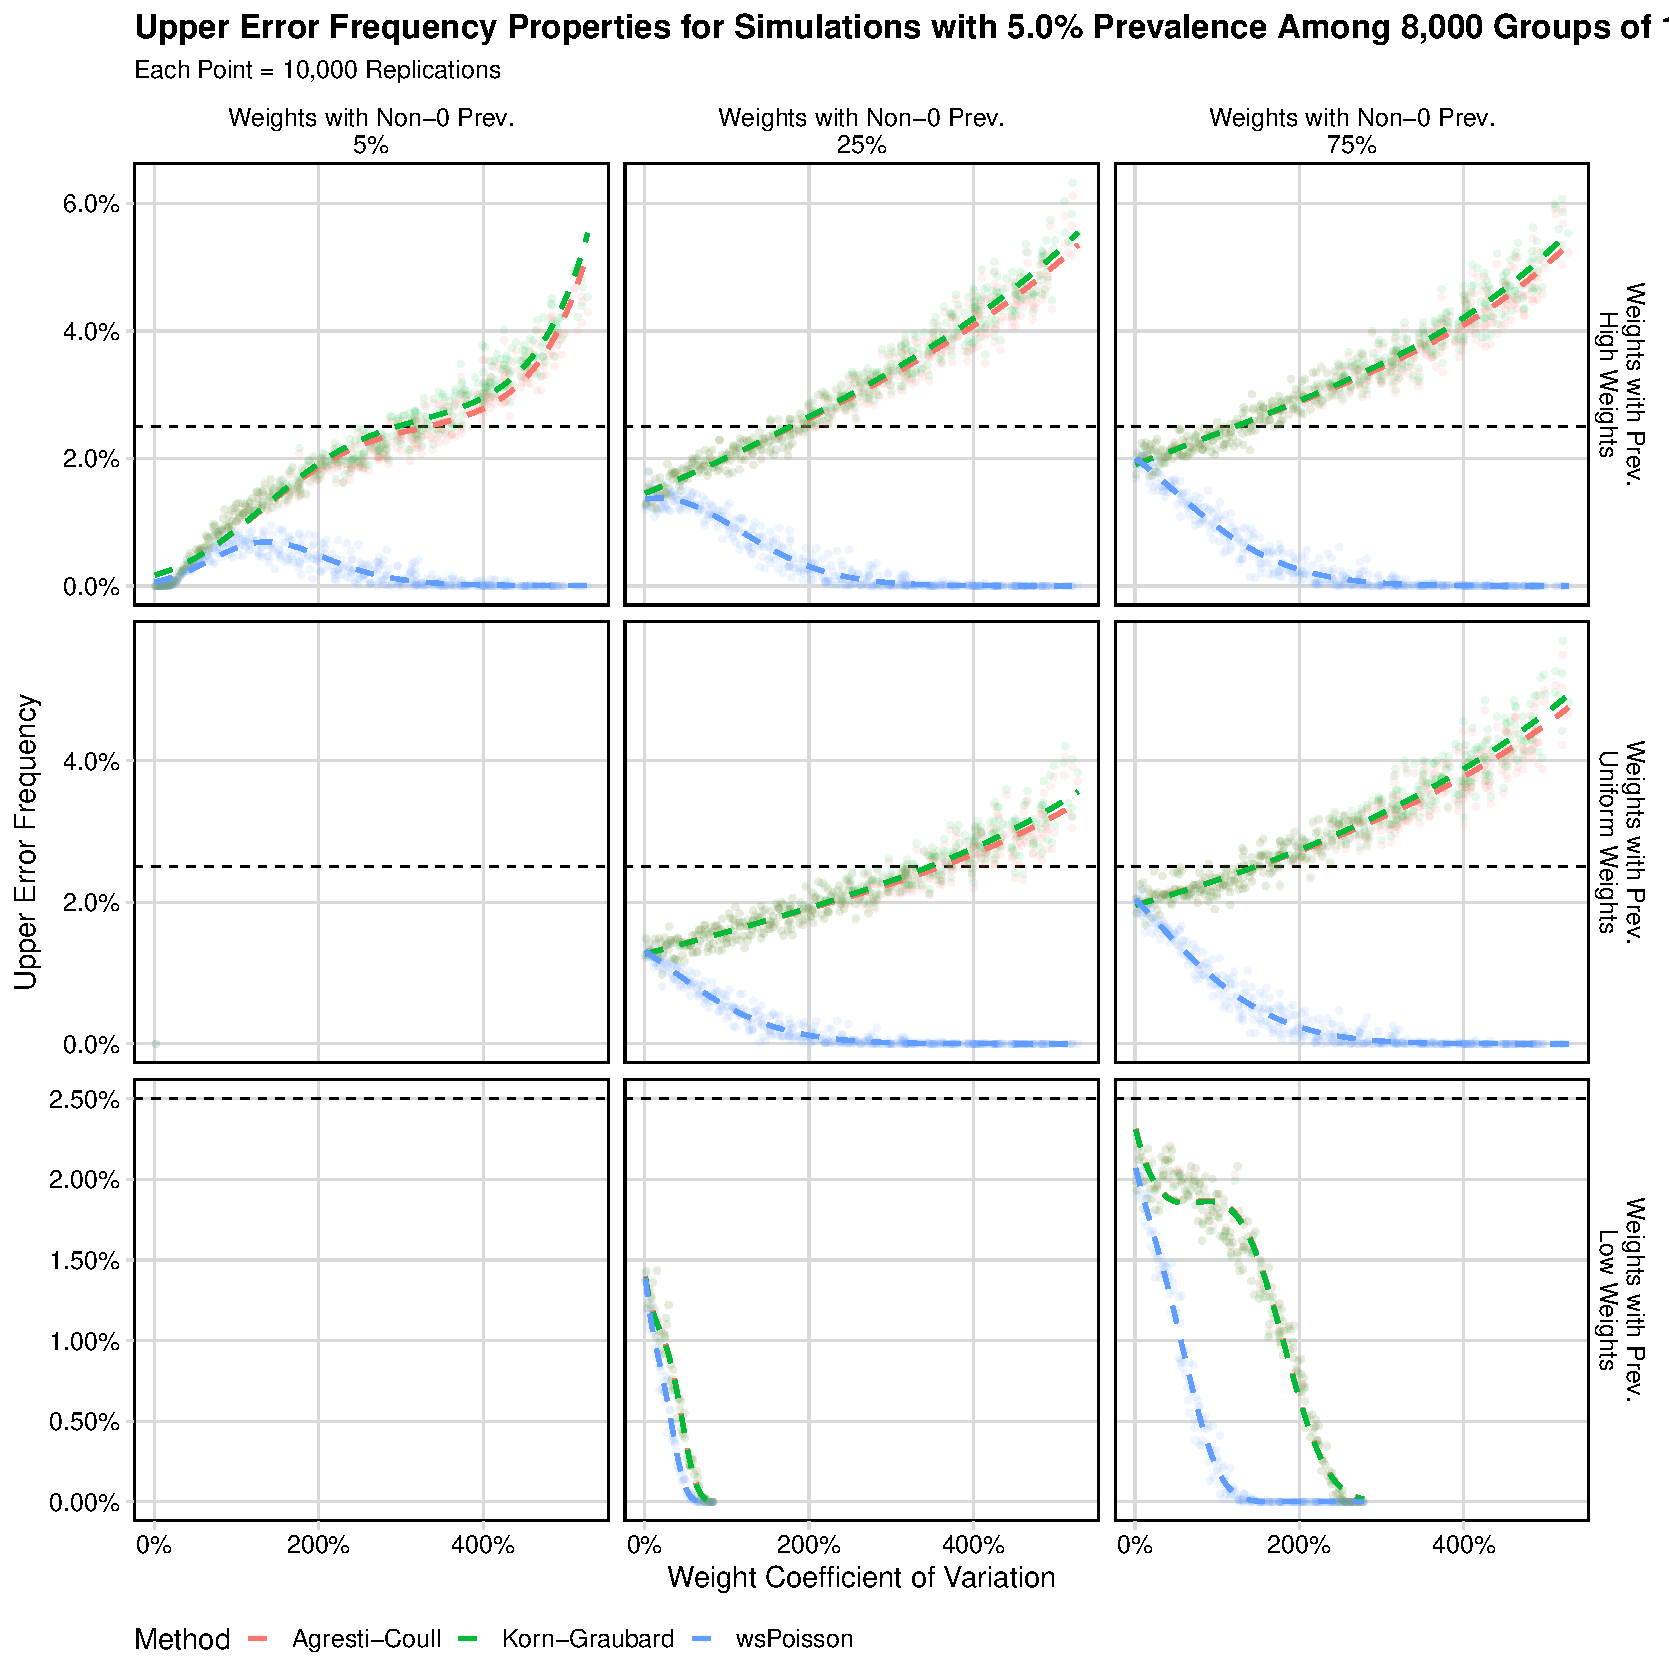
\includegraphics[width=0.8\textwidth]{perfect_upper_error_frequency_8000_groups_0_05_prev}
\caption{Upper error properties for the wsPoisson model and two standard methods, the Dean-Pagano modification of the Agresti-Coull method and of the Korn-Graubard method.
Each point represents 10,000 simulations of datasets from a population with 5\% prevalence, where 8000 individuals are sampled.
The horizontal dashed line indicates the nominal upper error rate, 2.5\%.
Colored dashed lines are estimates from a logistic regression model using quadratic splines.}
\label{ch_3:fig:perfect_upper_error_frequency_8000_groups_0_05_prev}
\end{figure}

\begin{figure}
\centering
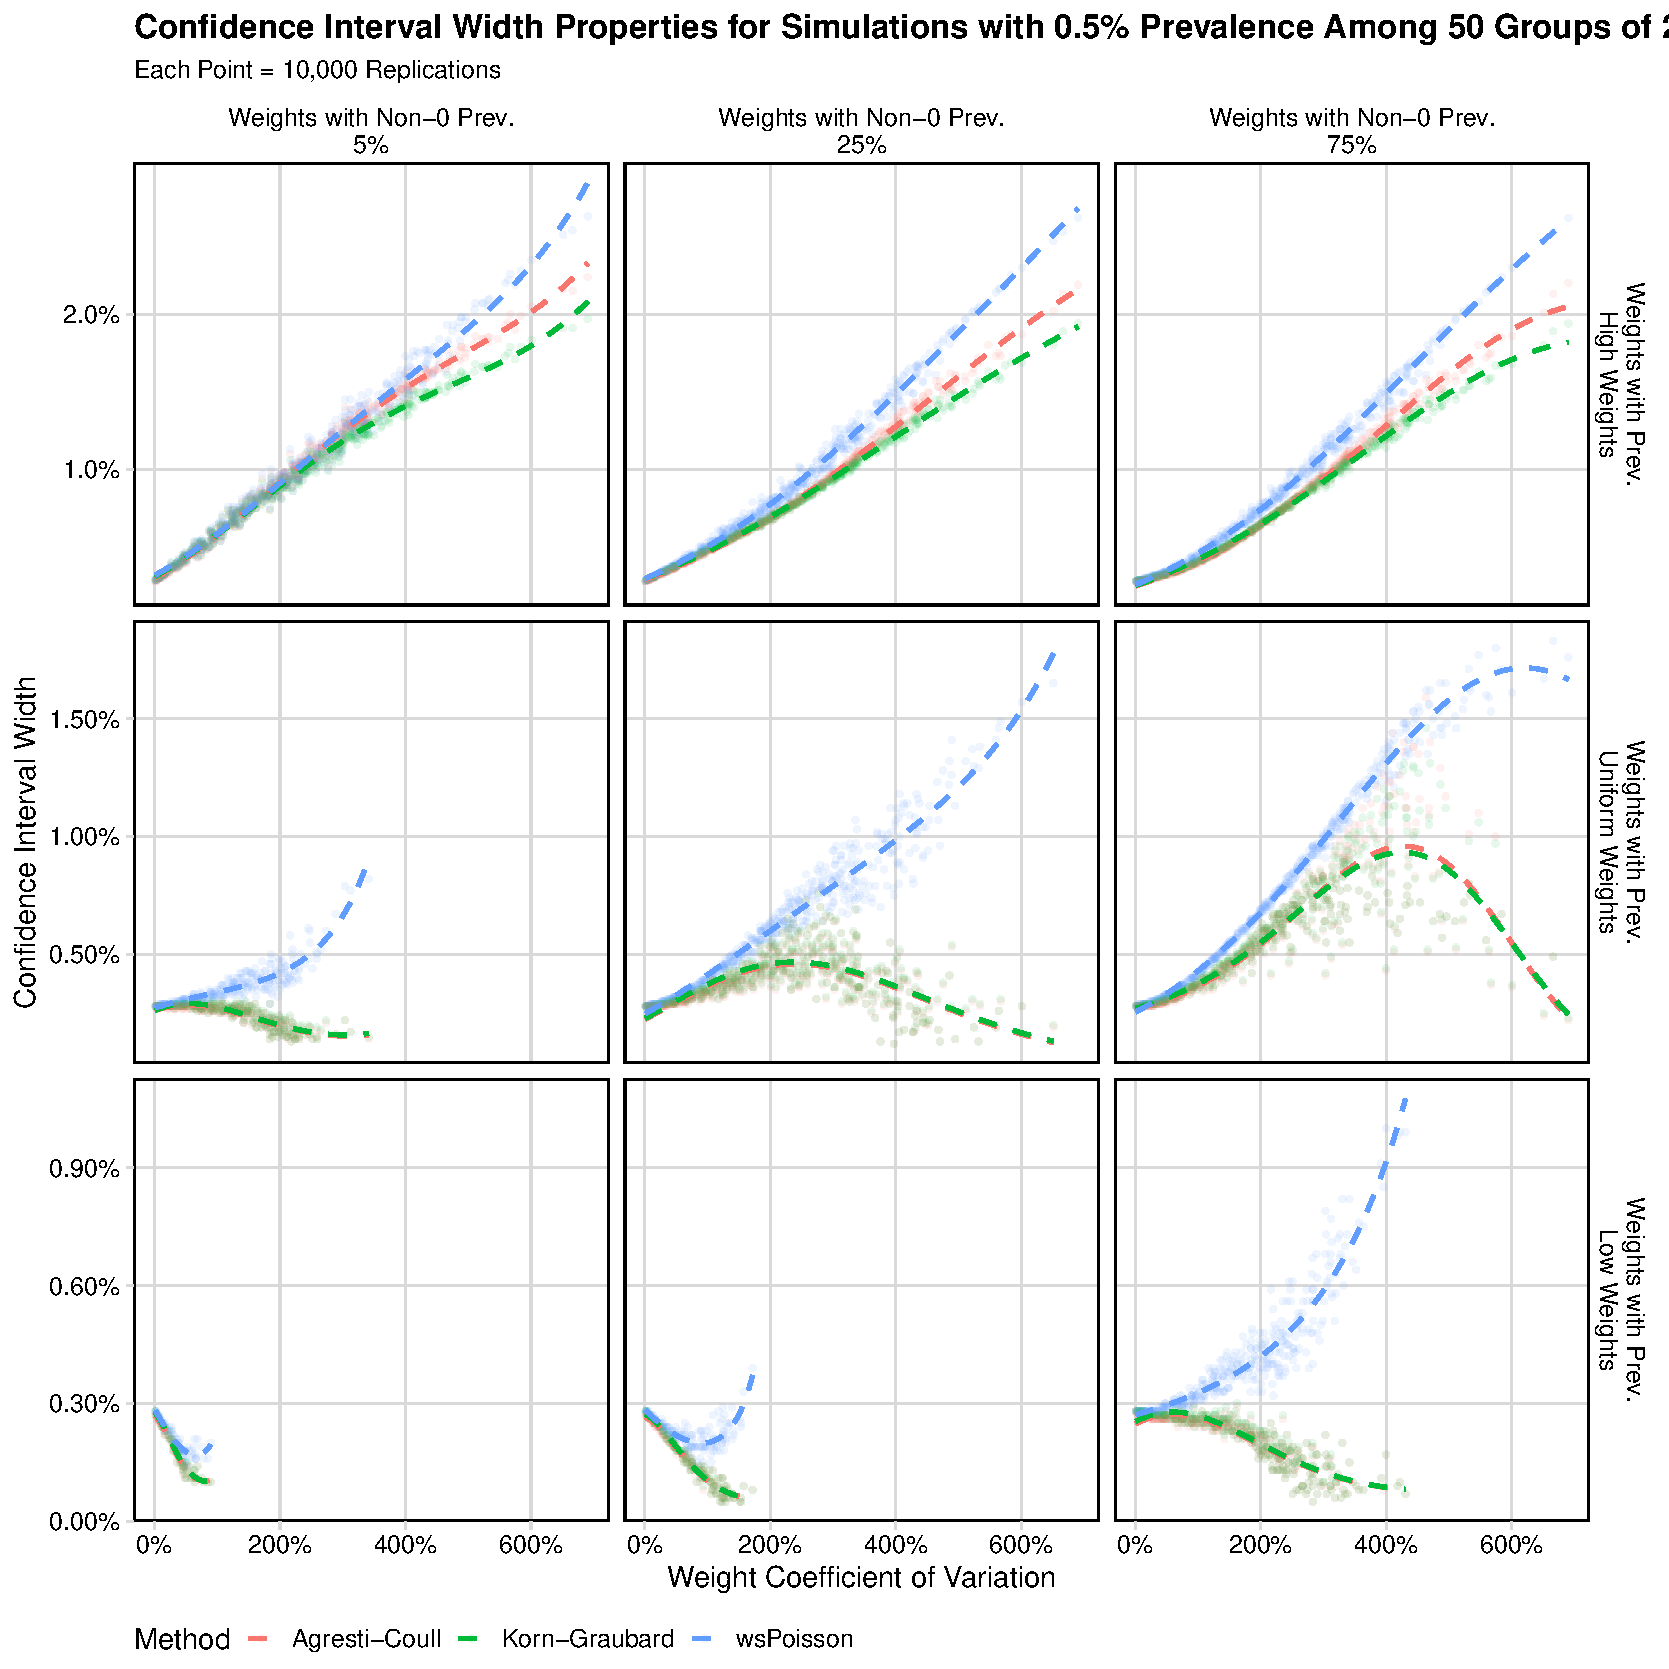
\includegraphics[width=0.8\textwidth]{perfect_confidence_interval_width_50_groups_0_005_prev}
\caption{Confidence interval width properties for the wsPoisson model and two standard methods, the Dean-Pagano modification of the Agresti-Coull method and of the Korn-Graubard method.
Each point represents 10,000 simulations of datasets from a population with 0.5\% prevalence, where 50 groups of 200 people are sampled.
Colored dashed lines are estimates from a logistic regression model using quadratic splines.}
\label{ch_3:fig:perfect_confidence_interval_width_50_groups_0_005_prev}
\end{figure}


\begin{figure}
\centering
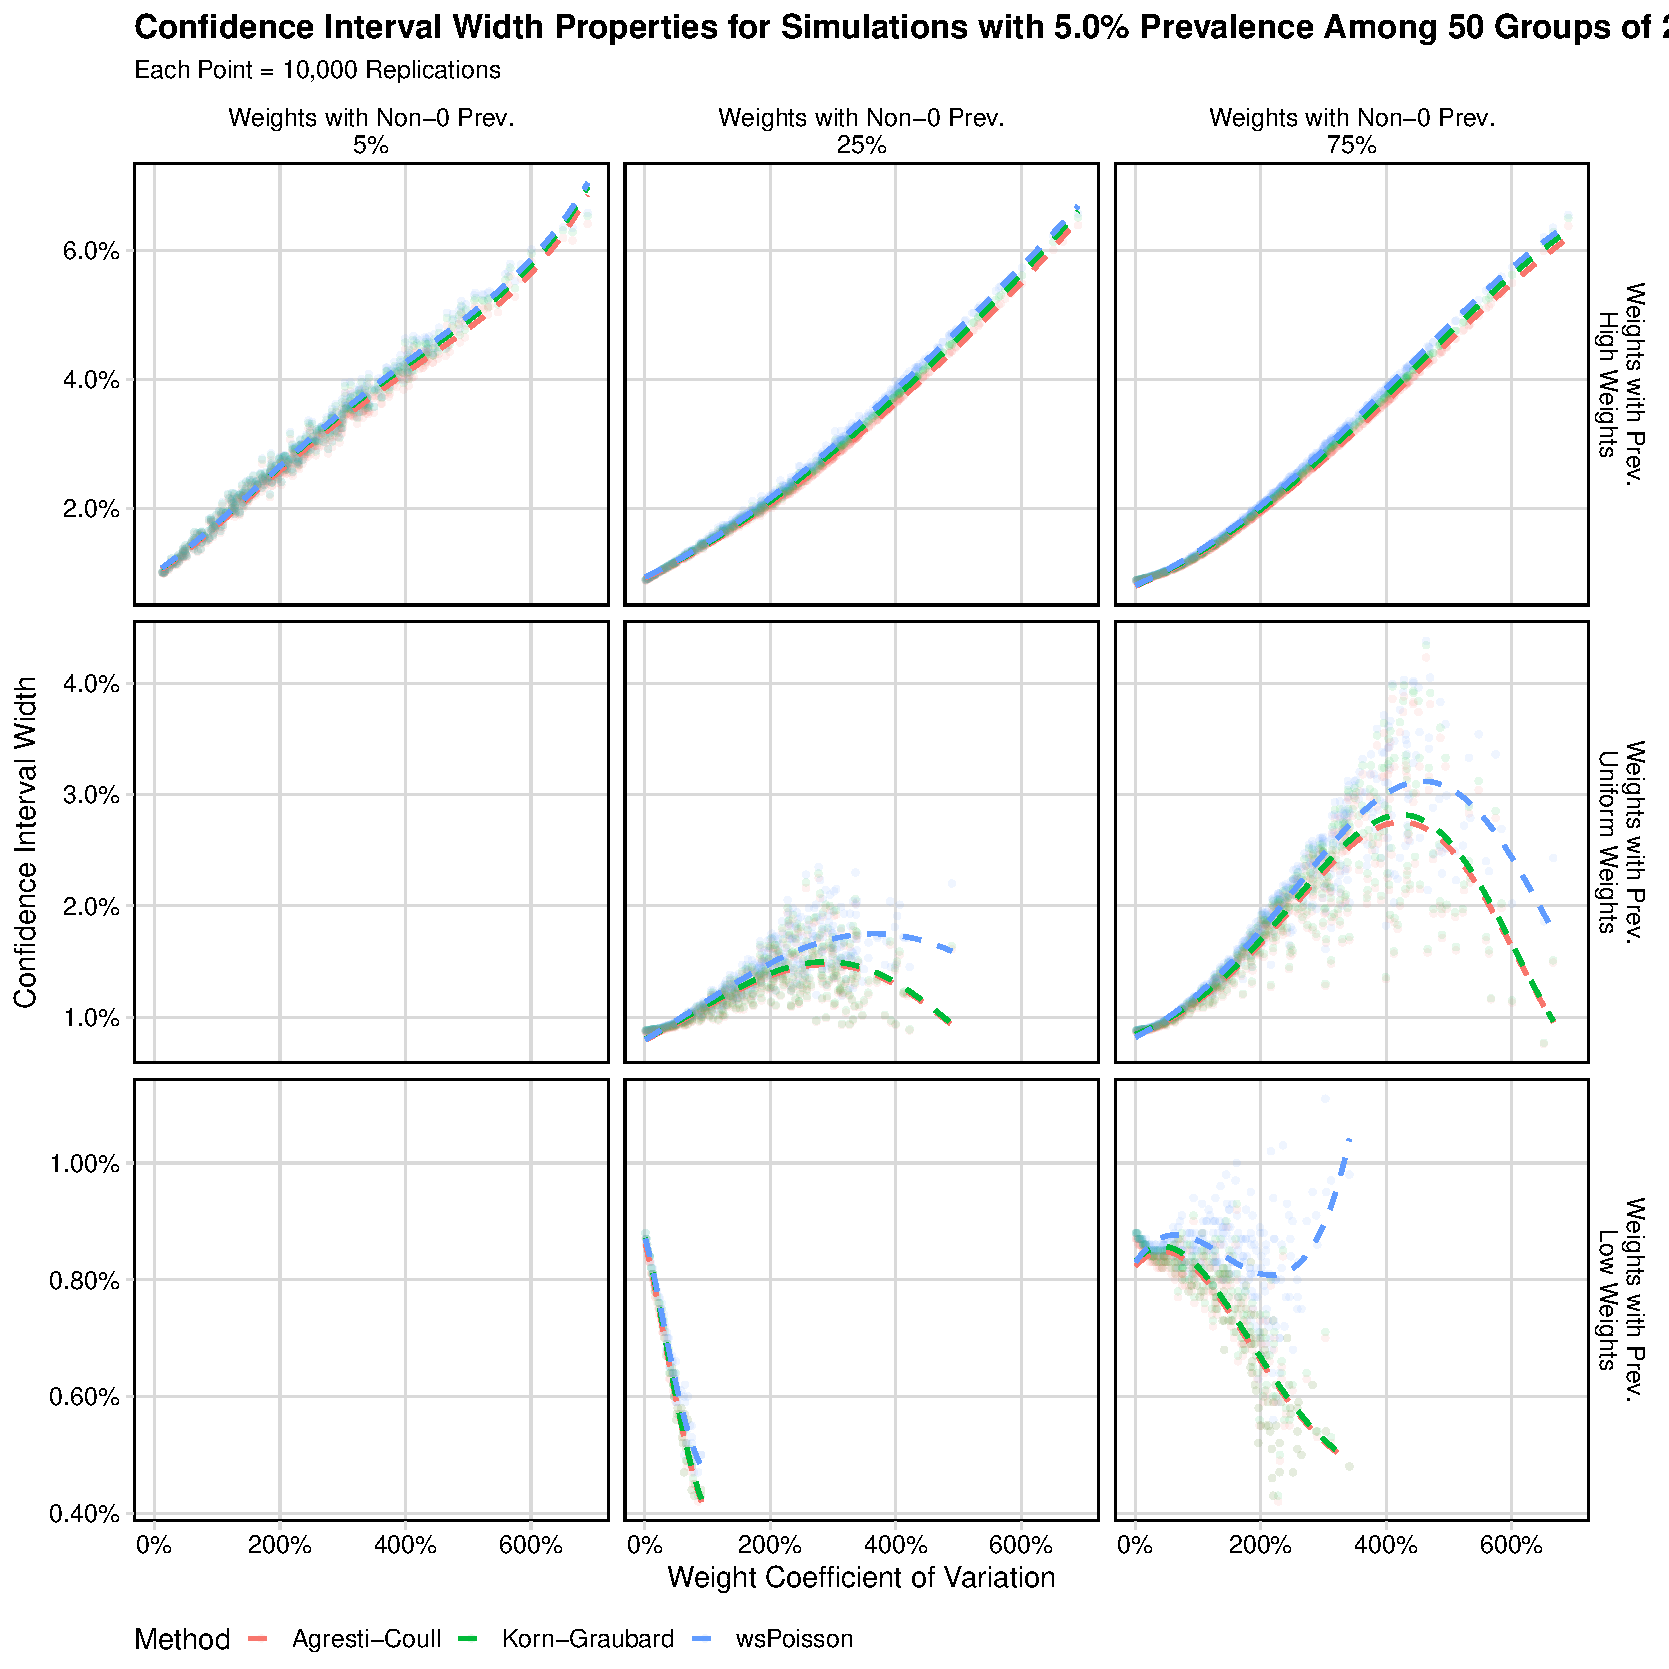
\includegraphics[width=0.8\textwidth]{perfect_confidence_interval_width_50_groups_0_05_prev}
\caption{Confidence interval width properties for the wsPoisson model and two standard methods, the Dean-Pagano modification of the Agresti-Coull method and of the Korn-Graubard method.
Each point represents 10,000 simulations of datasets from a population with 5\% prevalence, where 50 groups of 200 people are sampled.
Colored dashed lines are estimates from a logistic regression model using quadratic splines.}
\label{ch_3:fig:perfect_confidence_interval_width_50_groups_0_05_prev}
\end{figure}


\begin{figure}
\centering
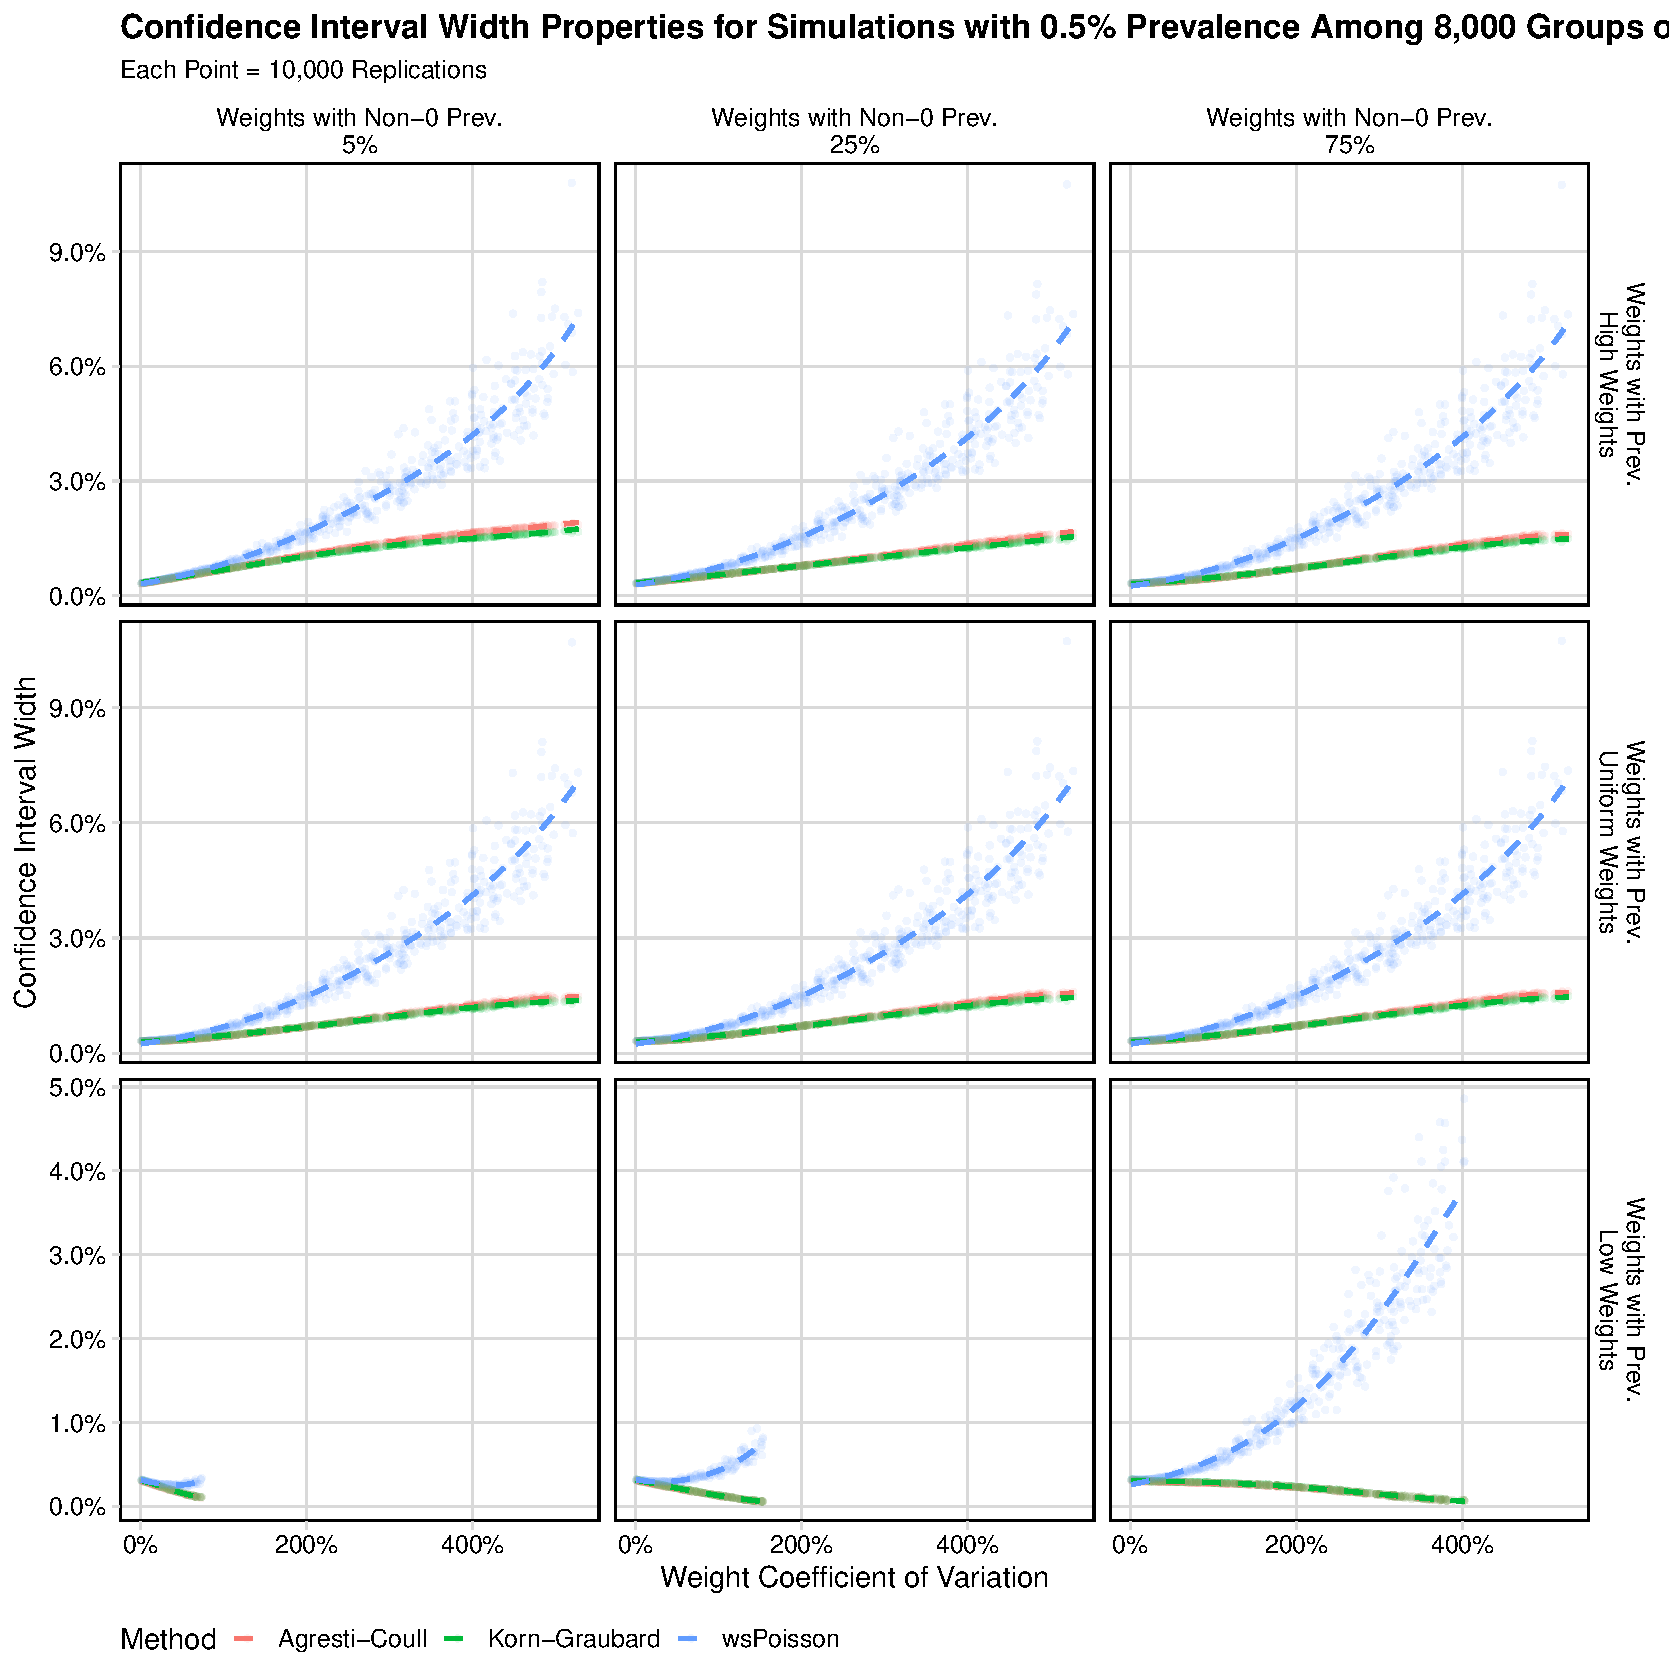
\includegraphics[width=0.8\textwidth]{perfect_confidence_interval_width_8000_groups_0_005_prev}
\caption{Confidence interval width properties for the wsPoisson model and two standard methods, the Dean-Pagano modification of the Agresti-Coull method and of the Korn-Graubard method.
Each point represents 10,000 simulations of datasets from a population with 0.5\% prevalence, where 8000 individuals are sampled.
Colored dashed lines are estimates from a logistic regression model using quadratic splines.}
\label{ch_3:fig:perfect_confidence_interval_width_8000_groups_0_005_prev}
\end{figure}


\begin{figure}
\centering
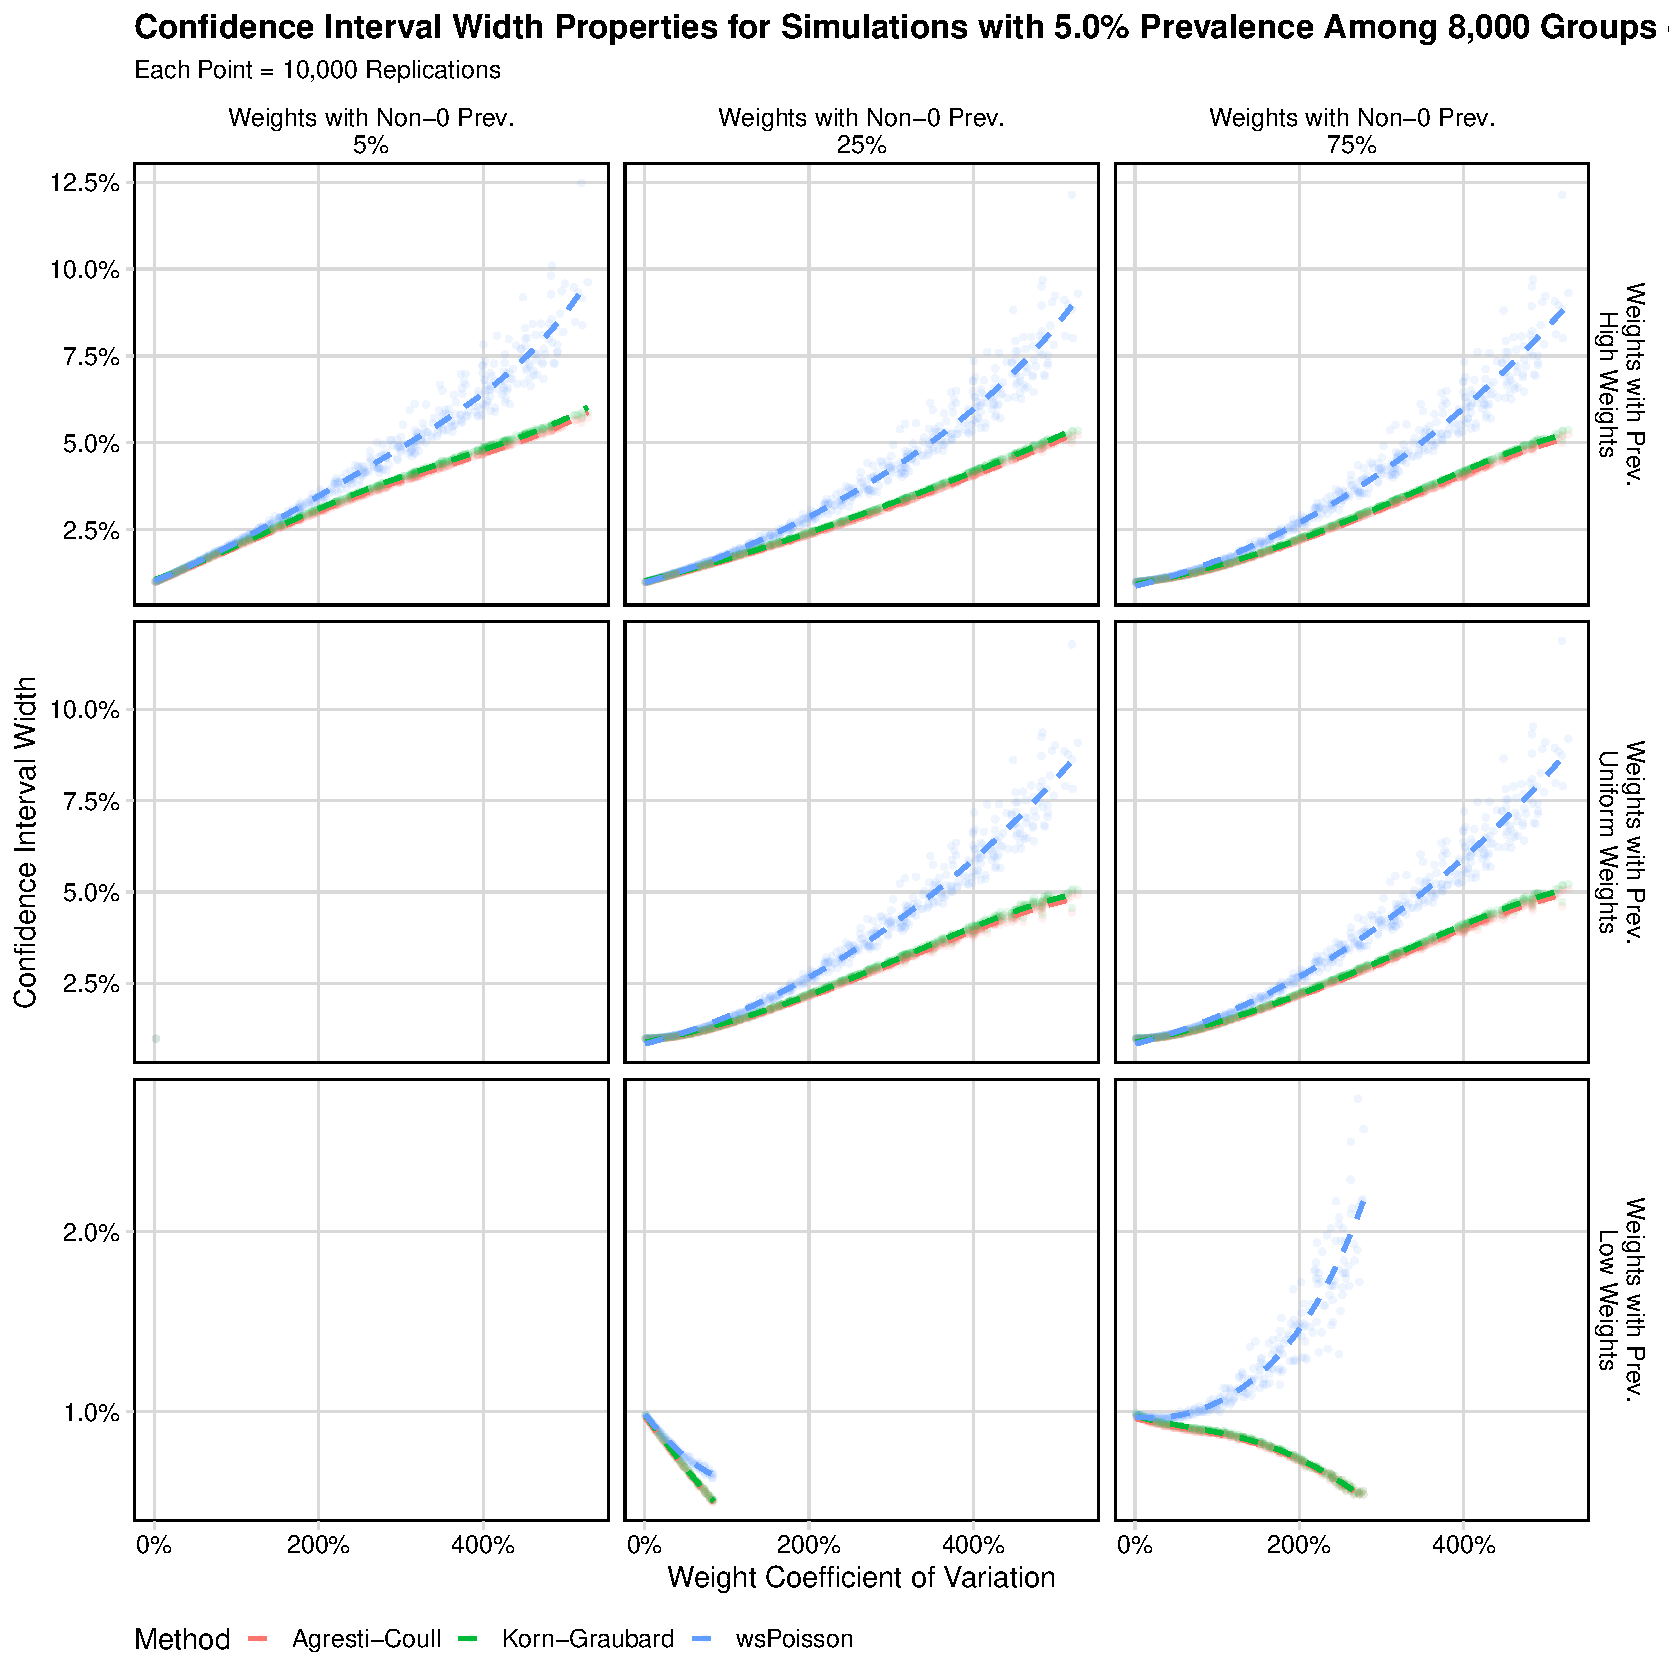
\includegraphics[width=0.8\textwidth]{perfect_confidence_interval_width_8000_groups_0_05_prev}
\caption{Confidence interval width properties for the wsPoisson model and two standard methods, the Dean-Pagano modification of the Agresti-Coull method and of the Korn-Graubard method.
Each point represents 10,000 simulations of datasets from a population with 5\% prevalence, where 8000 individuals are sampled.
Colored dashed lines are estimates from a logistic regression model using quadratic splines.}
\label{ch_3:fig:perfect_confidence_interval_width_8000_groups_0_05_prev}
\end{figure}

% Start of Imperfect

\begin{figure}
\centering
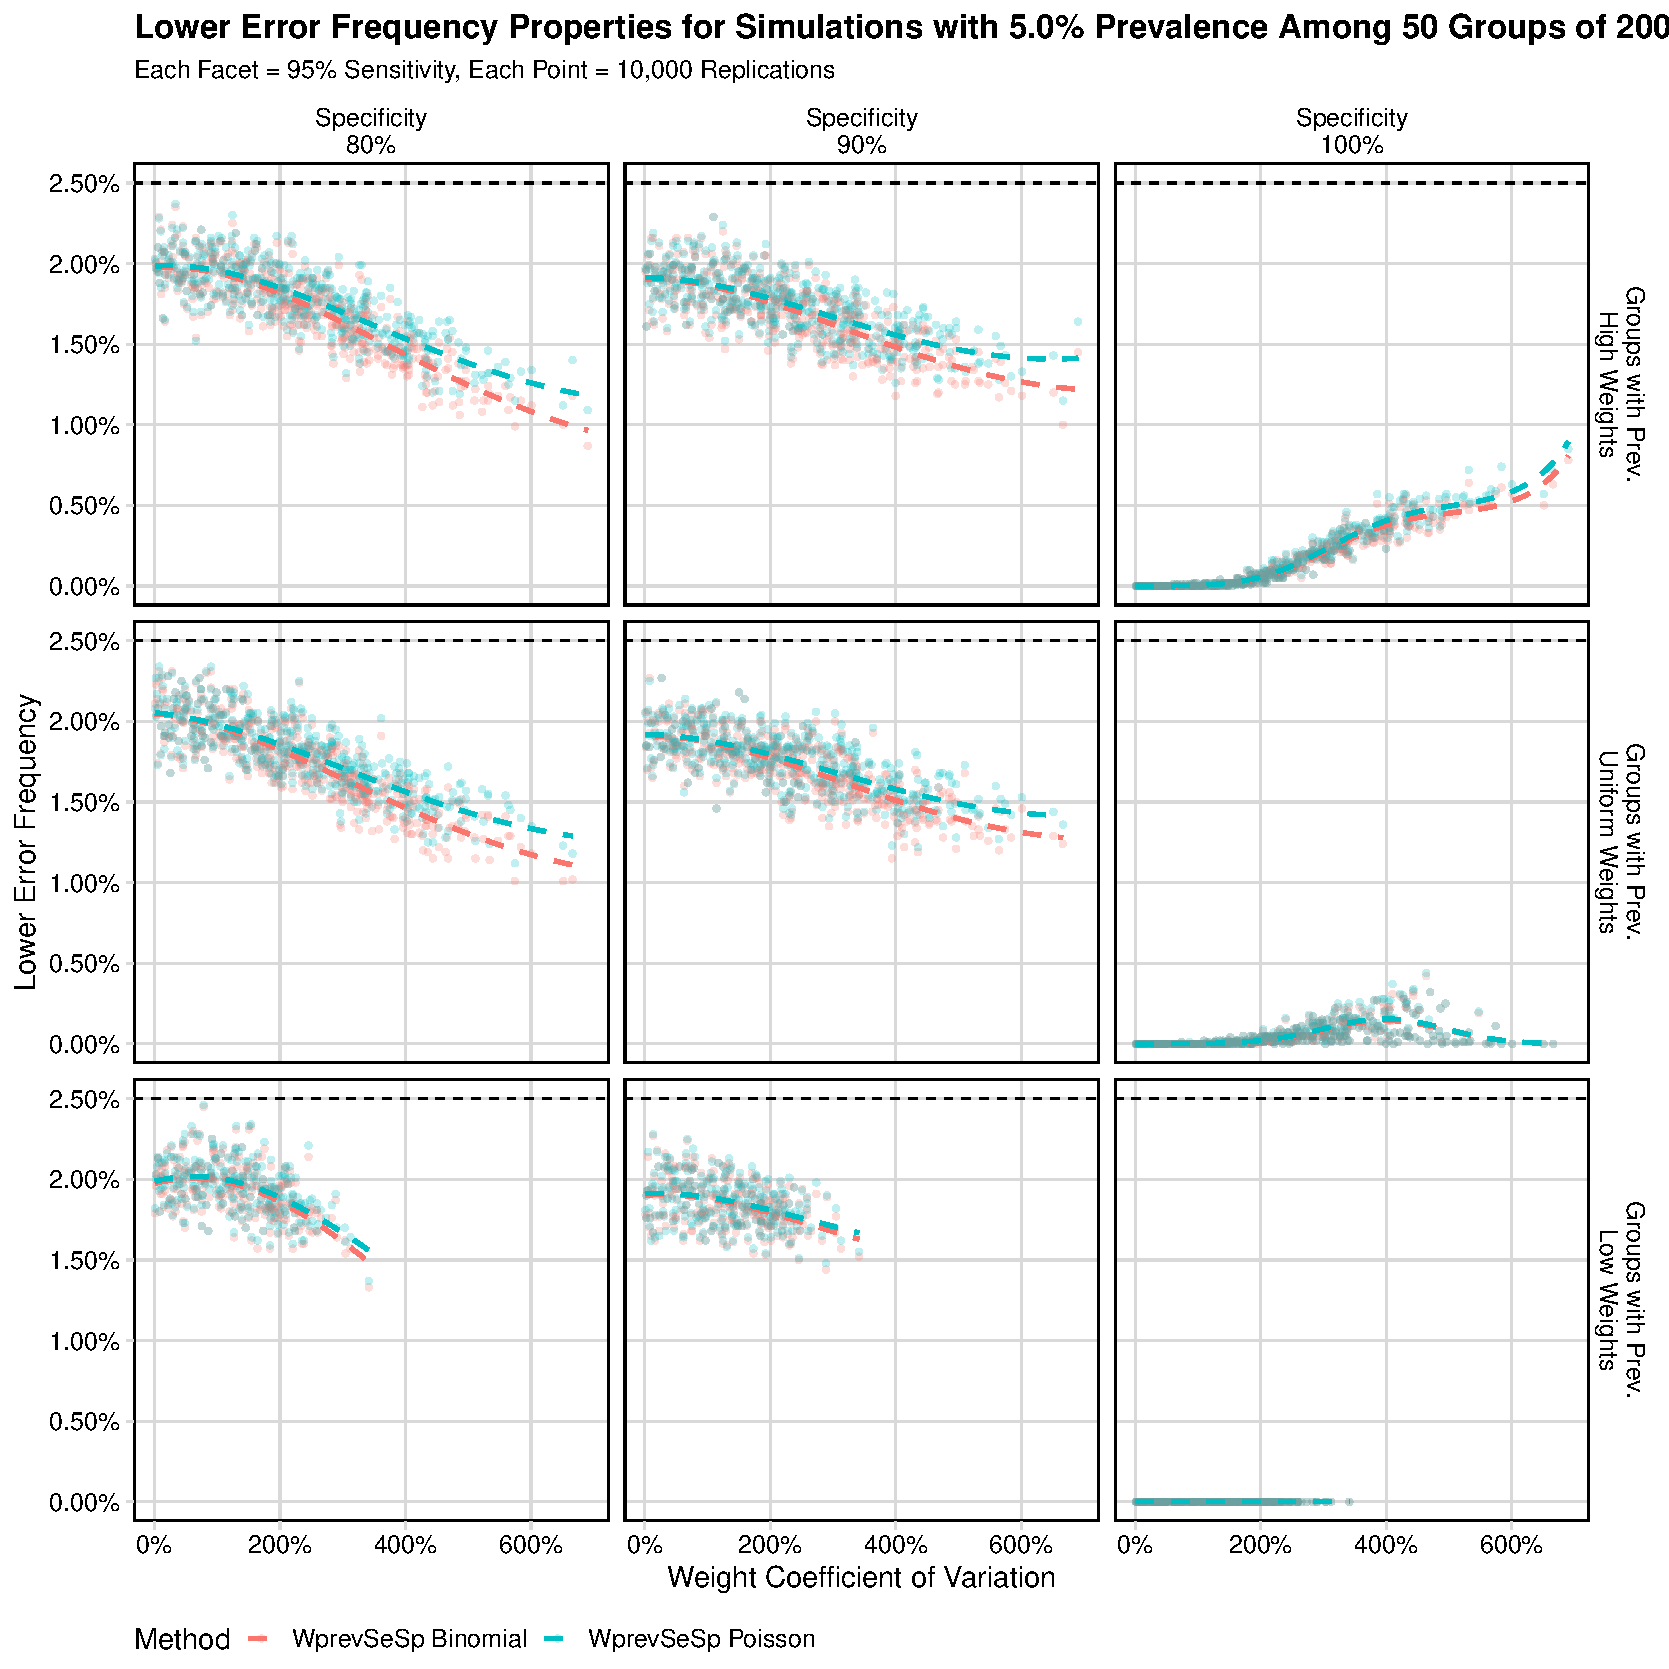
\includegraphics[width=0.8\textwidth]{imperfect_lower_error_frequency_50_groups_0_05_prev}
\caption{Lower error properties for the confidence interval procedures, WprevSeSp Binomial and WprevSeSp Poisson.
Each point represents 10,000 simulations of datasets from a population with 0.5\% prevalence, where 50 groups of 200 people are sampled.
Each dataset also includes simulated results of tests to evaluate the sensitivity and specificity of the assay performed on 60 and 300 individuals, respectively.
The horizontal dashed line indicates the nominal lower error rate, 2.5\%.
Colored dashed lines are estimates from a logistic regression model using quadratic splines. If the WprevSeSp Binomial line is not visible, then it is covered by the WprevSeSp Poisson line.}
\label{ch_3:fig:imperfect_lower_error_frequency_50_groups_0_05_prev}
\end{figure}

\begin{figure}
\centering
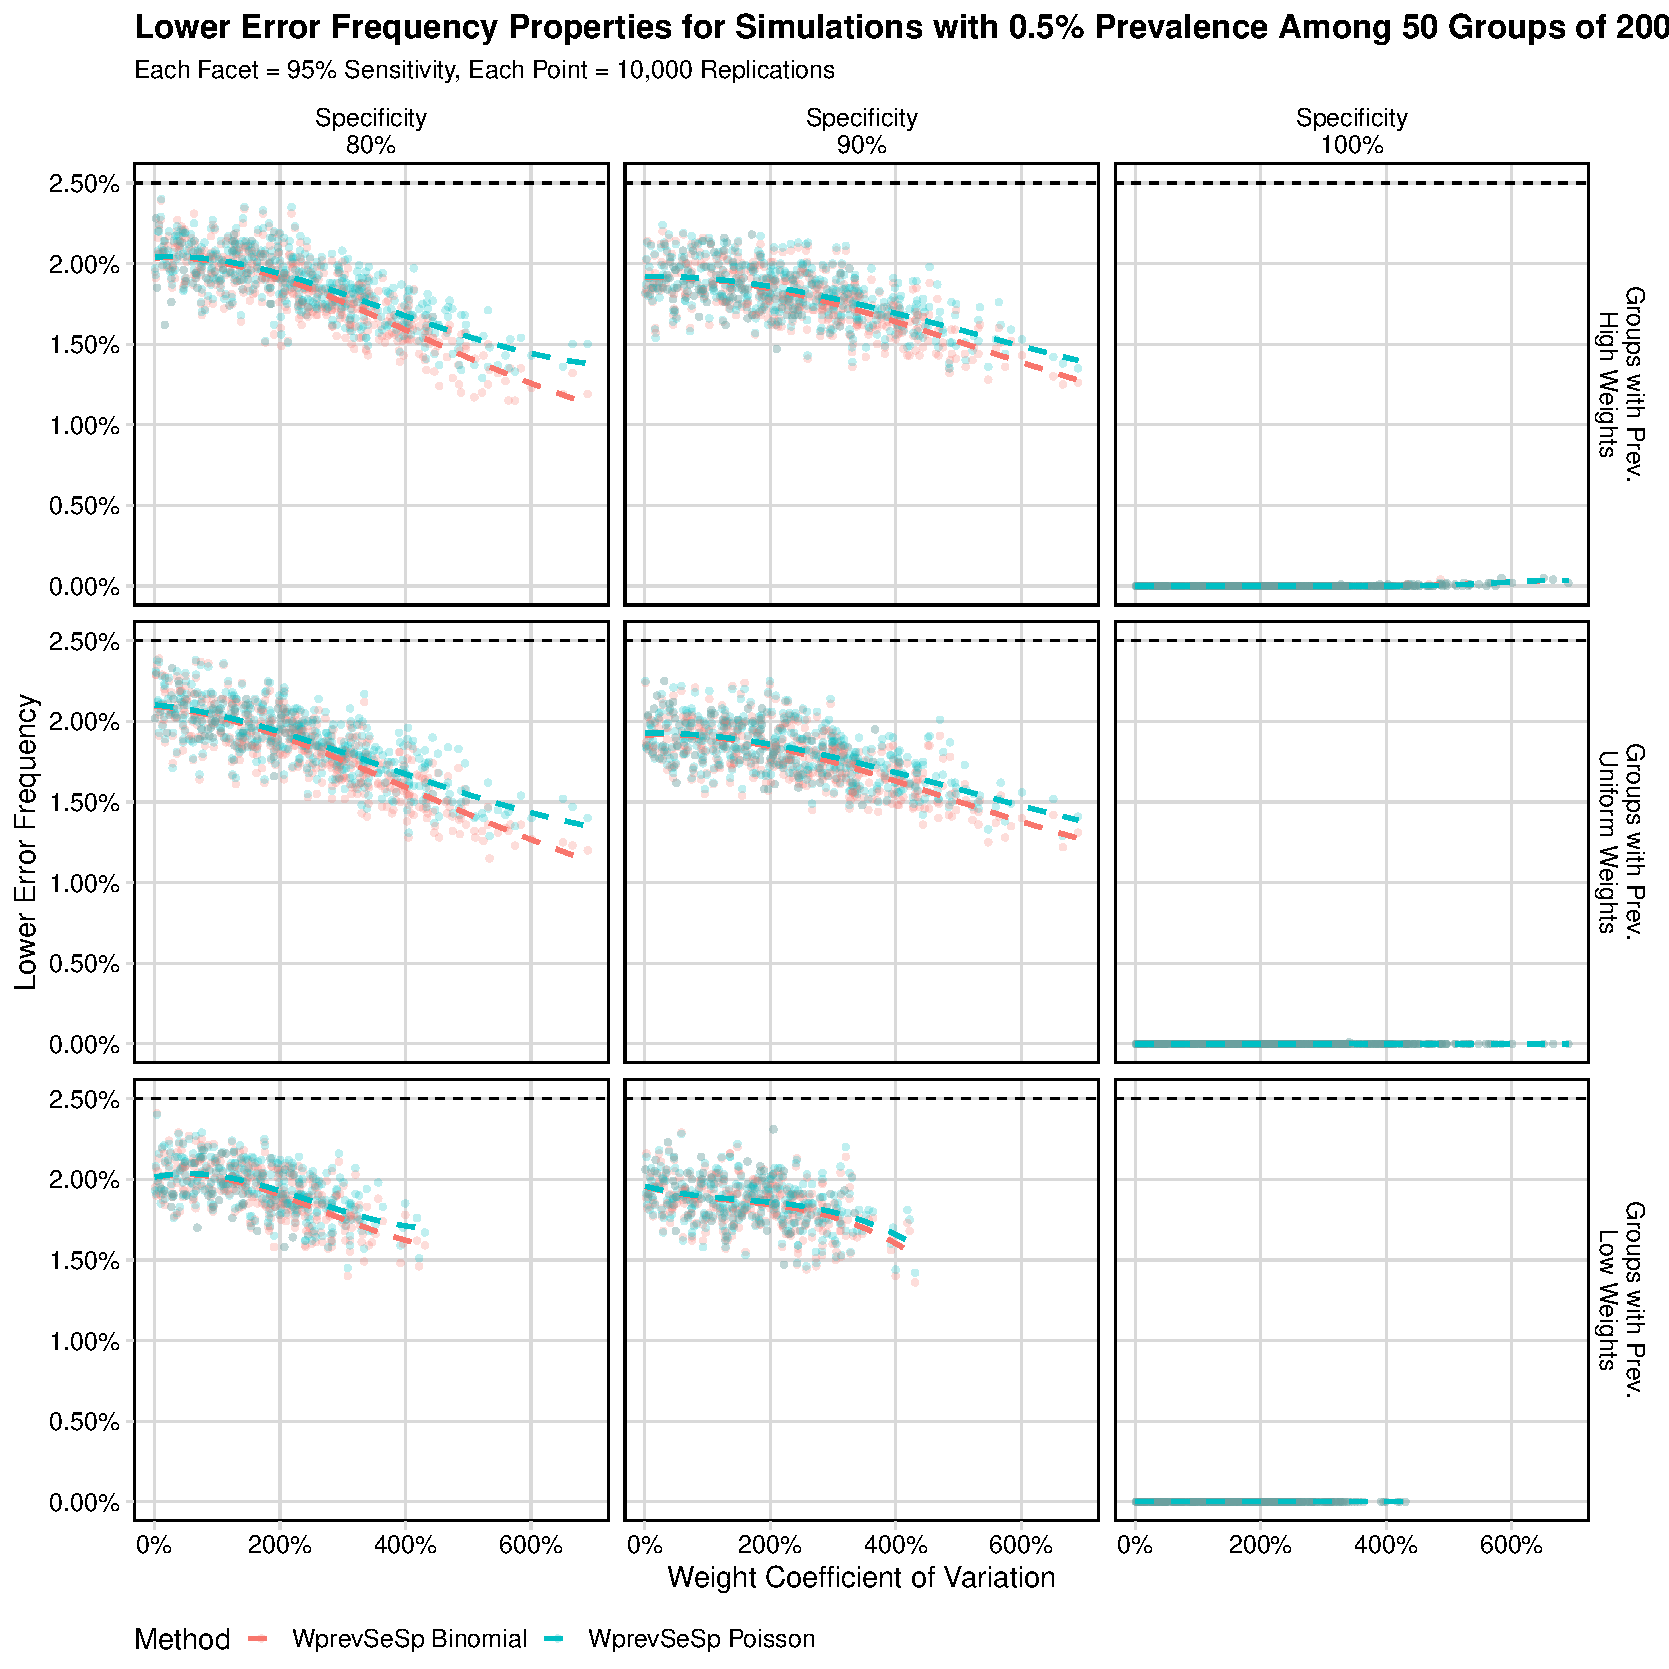
\includegraphics[width=0.8\textwidth]{imperfect_lower_error_frequency_50_groups_0_005_prev}
\caption{Lower error properties for the confidence interval procedures, WprevSeSp Binomial and WprevSeSp Poisson.
Each point represents 10,000 simulations of datasets from a population with 0.5\% prevalence, where 8000 individuals are sampled.
Each dataset also includes simulated results of tests to evaluate the sensitivity and specificity of the assay performed on 60 and 300 individuals, respectively.
The horizontal dashed line indicates the nominal lower error rate, 2.5\%.
Colored dashed lines are estimates from a logistic regression model using quadratic splines.}
\label{ch_3:fig:imperfect_lower_error_frequency_50_groups_0_005_prev}
\end{figure}

\begin{figure}
\centering
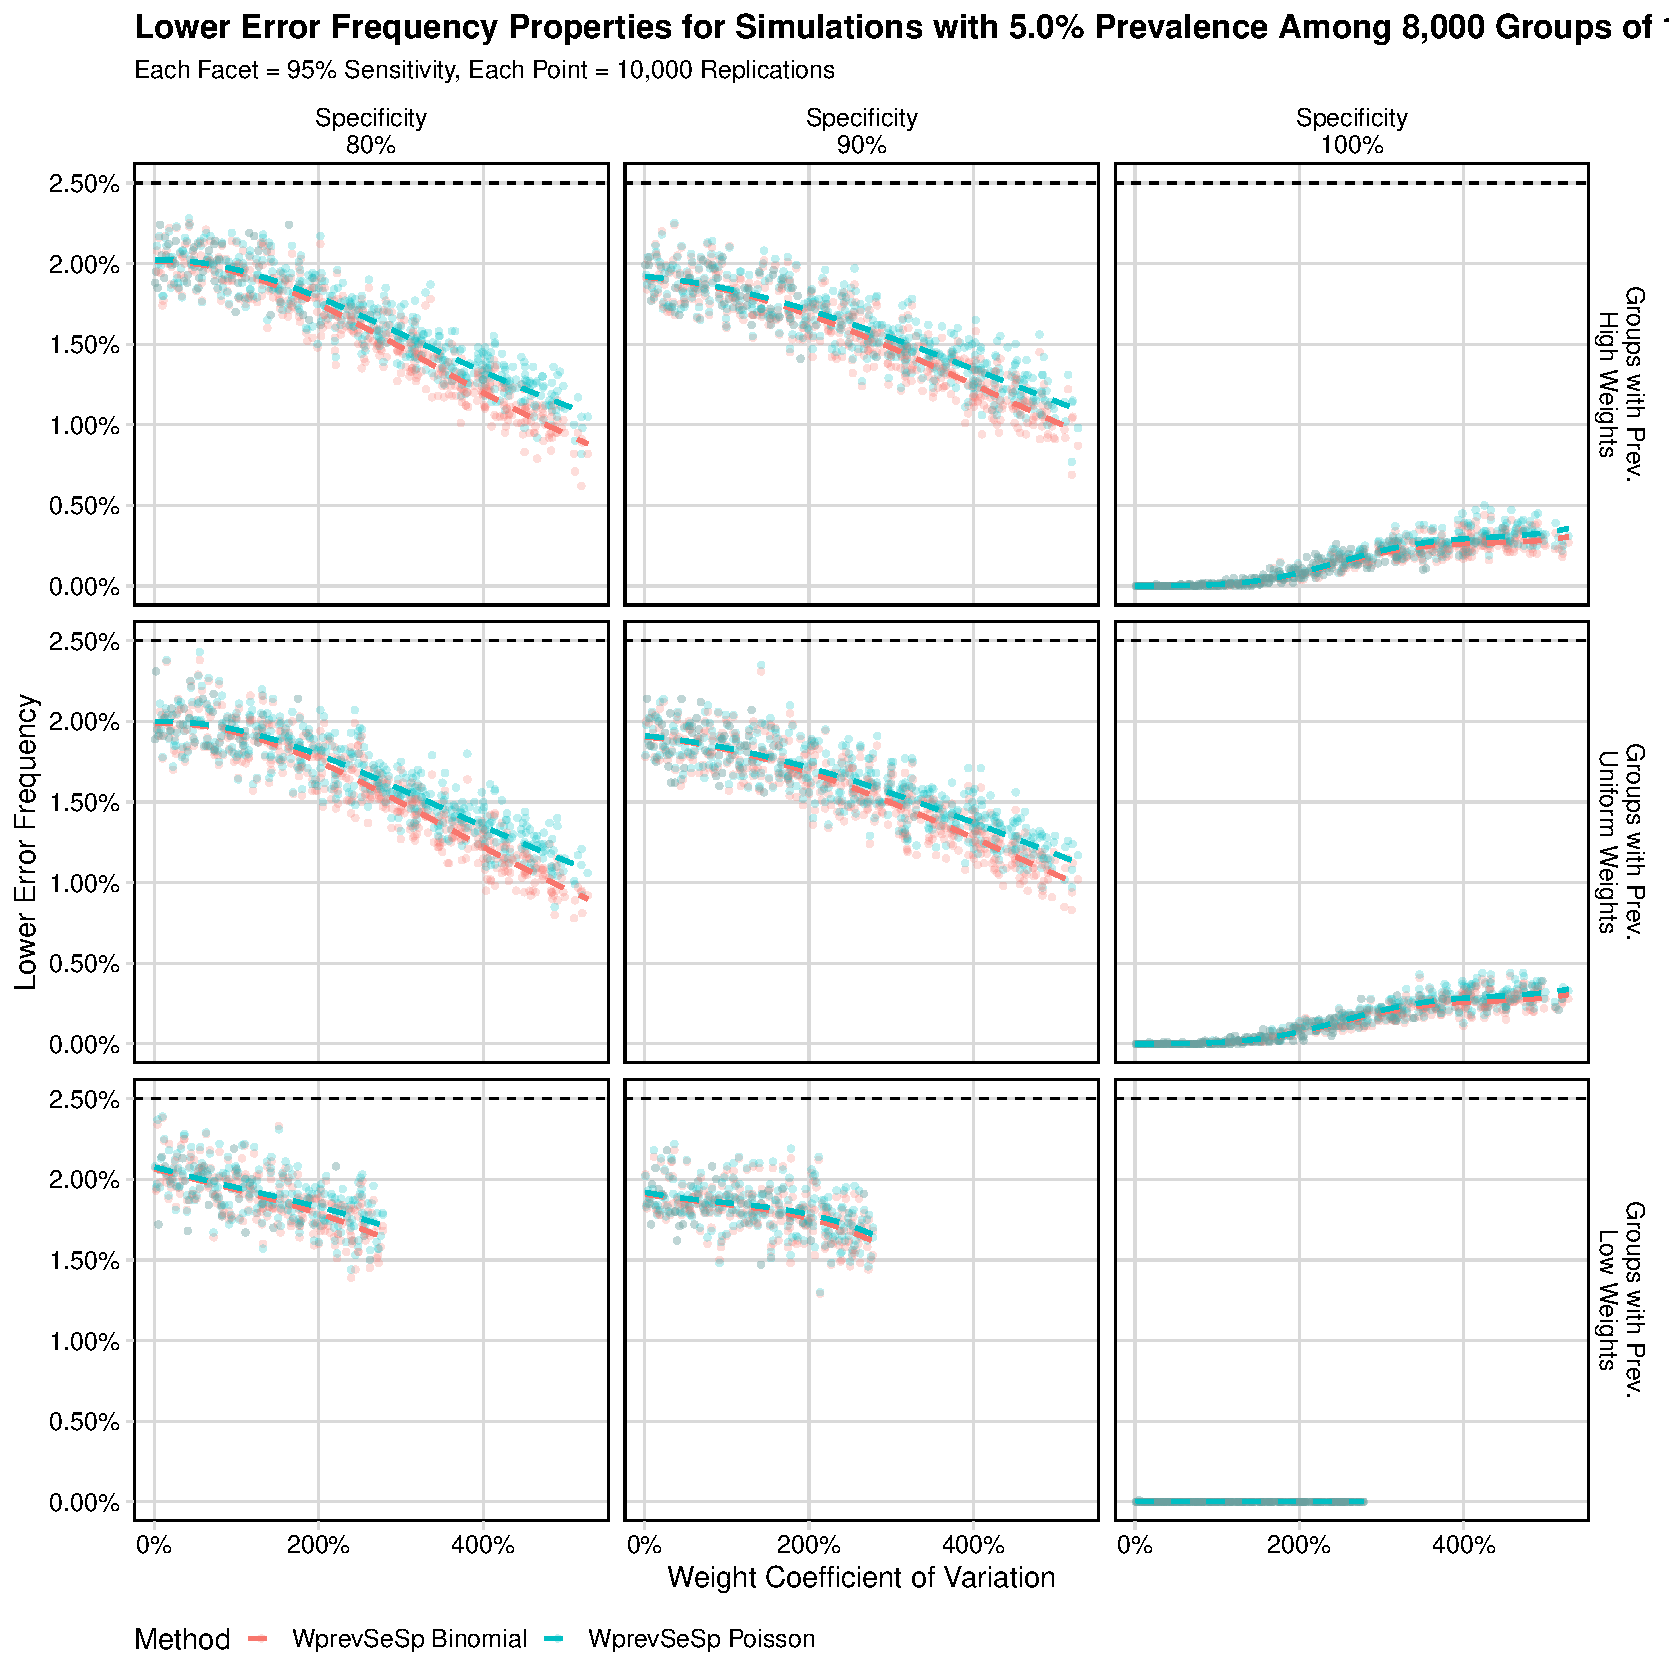
\includegraphics[width=0.8\textwidth]{imperfect_lower_error_frequency_8000_groups_0_05_prev}
\caption{Lower error properties for the confidence interval procedures, WprevSeSp Binomial and WprevSeSp Poisson.
Each point represents 10,000 simulations of datasets from a population with 5\% prevalence, where 50 groups of 200 people are sampled.
Each dataset also includes simulated results of tests to evaluate the sensitivity and specificity of the assay performed on 60 and 300 individuals, respectively.
The horizontal dashed line indicates the nominal lower error rate, 2.5\%.
Colored dashed lines are estimates from a logistic regression model using quadratic splines.}
\label{ch_3:fig:imperfect_lower_error_frequency_8000_groups_0_05_prev}
\end{figure}

\begin{figure}
\centering
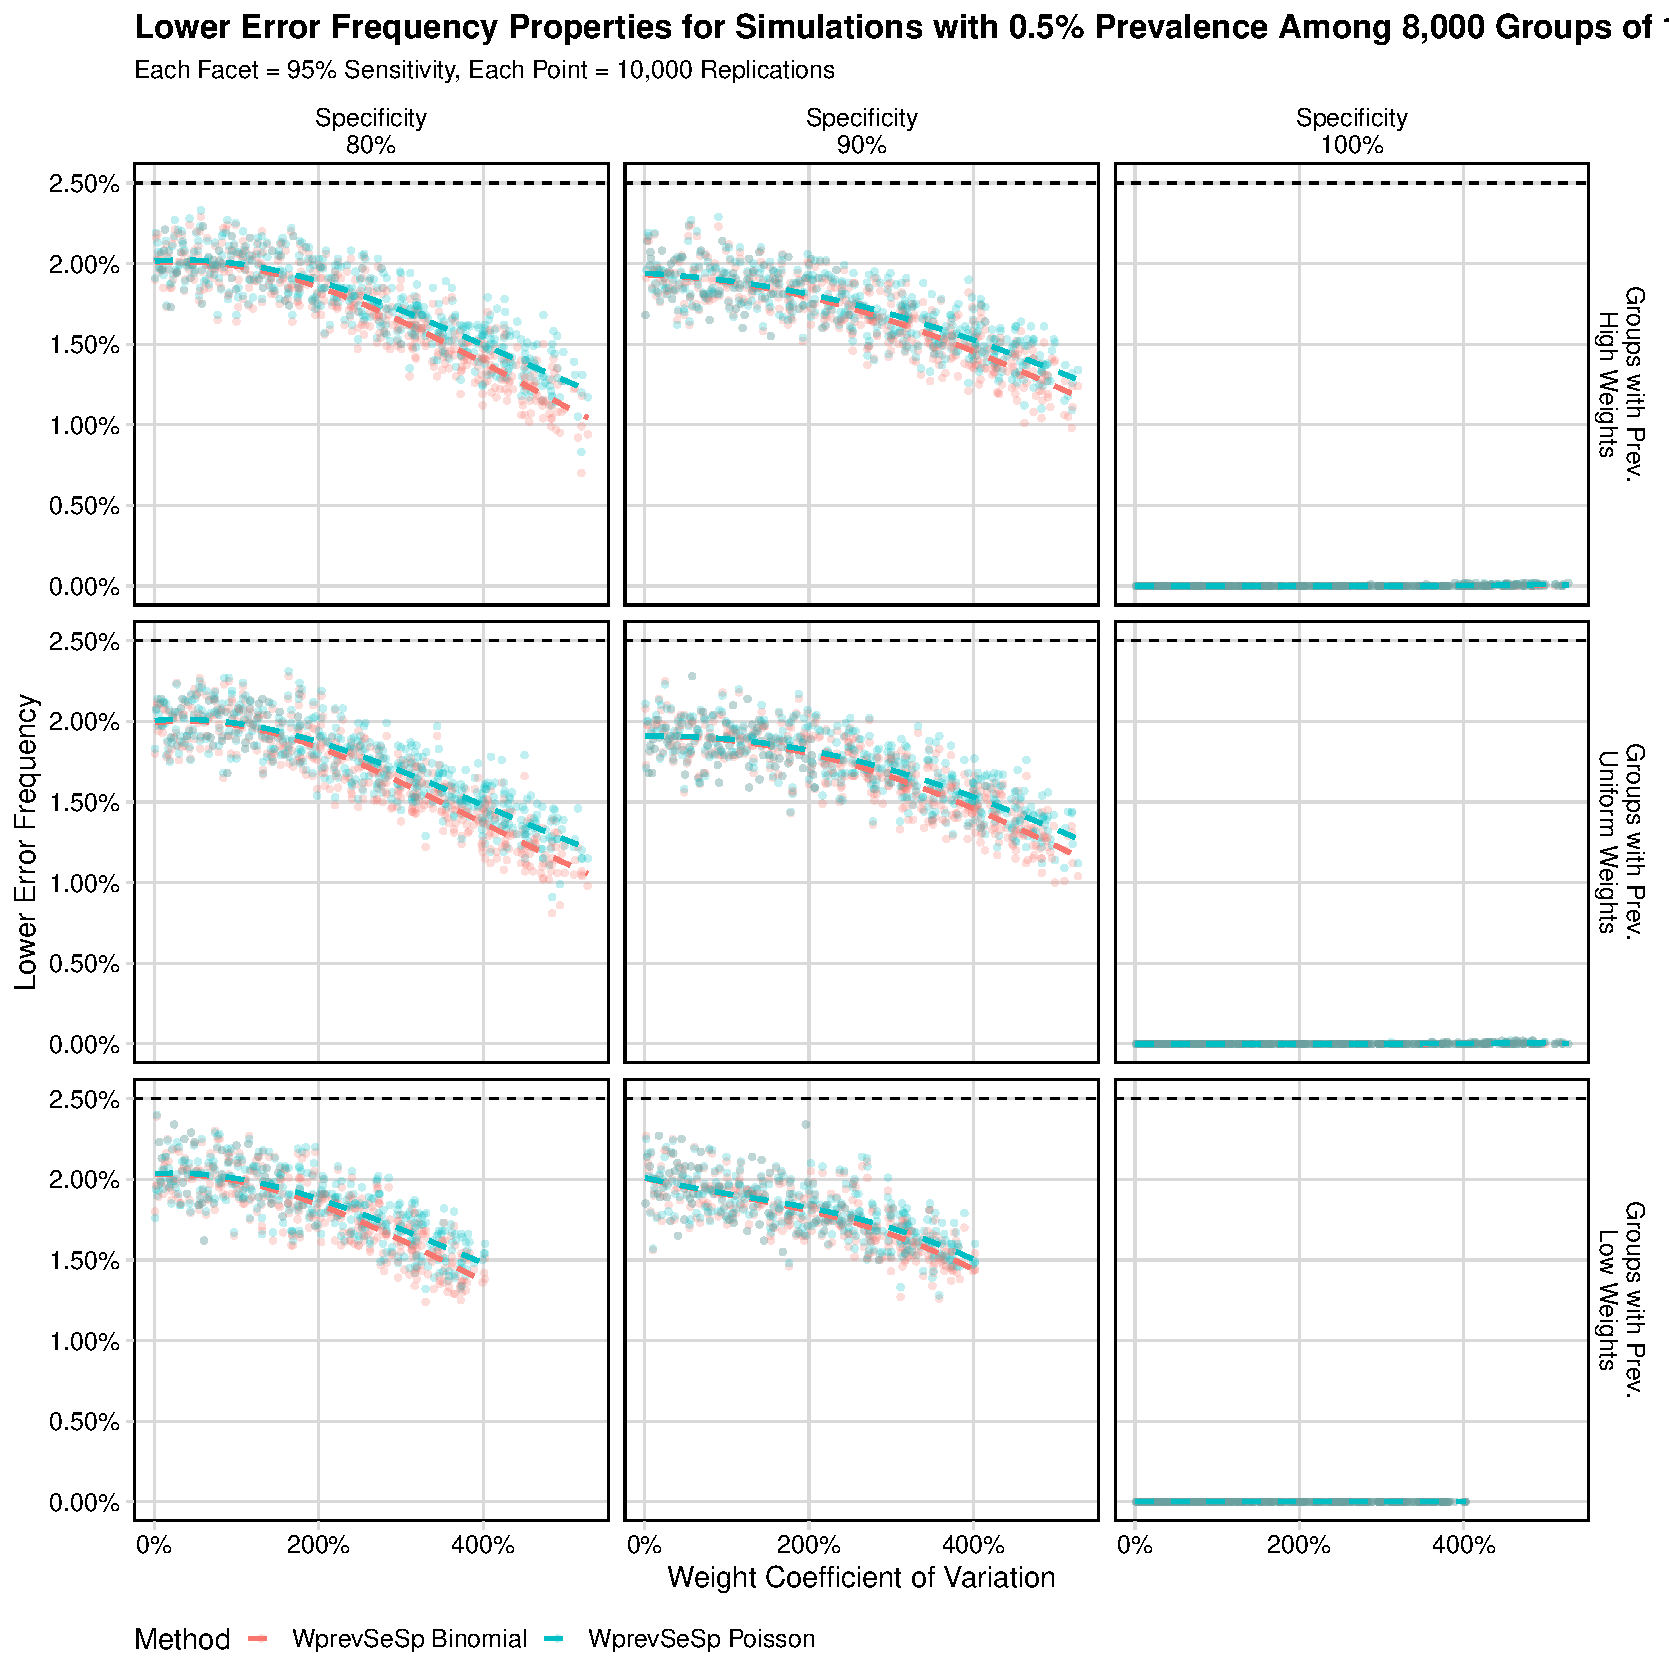
\includegraphics[width=0.8\textwidth]{imperfect_lower_error_frequency_8000_groups_0_005_prev}
\caption{Lower error properties for the confidence interval procedures, WprevSeSp Binomial and WprevSeSp Poisson.
Each point represents 10,000 simulations of datasets from a population with 5\% prevalence, where 8000 individuals are sampled.
Each dataset also includes simulated results of tests to evaluate the sensitivity and specificity of the assay performed on 60 and 300 individuals, respectively.
The horizontal dashed line indicates the nominal lower error rate, 2.5\%.
Colored dashed lines are estimates from a logistic regression model using quadratic splines.}
\label{ch_3:fig:imperfect_lower_error_frequency_8000_groups_0_005_prev}
\end{figure}

\begin{figure}
\centering
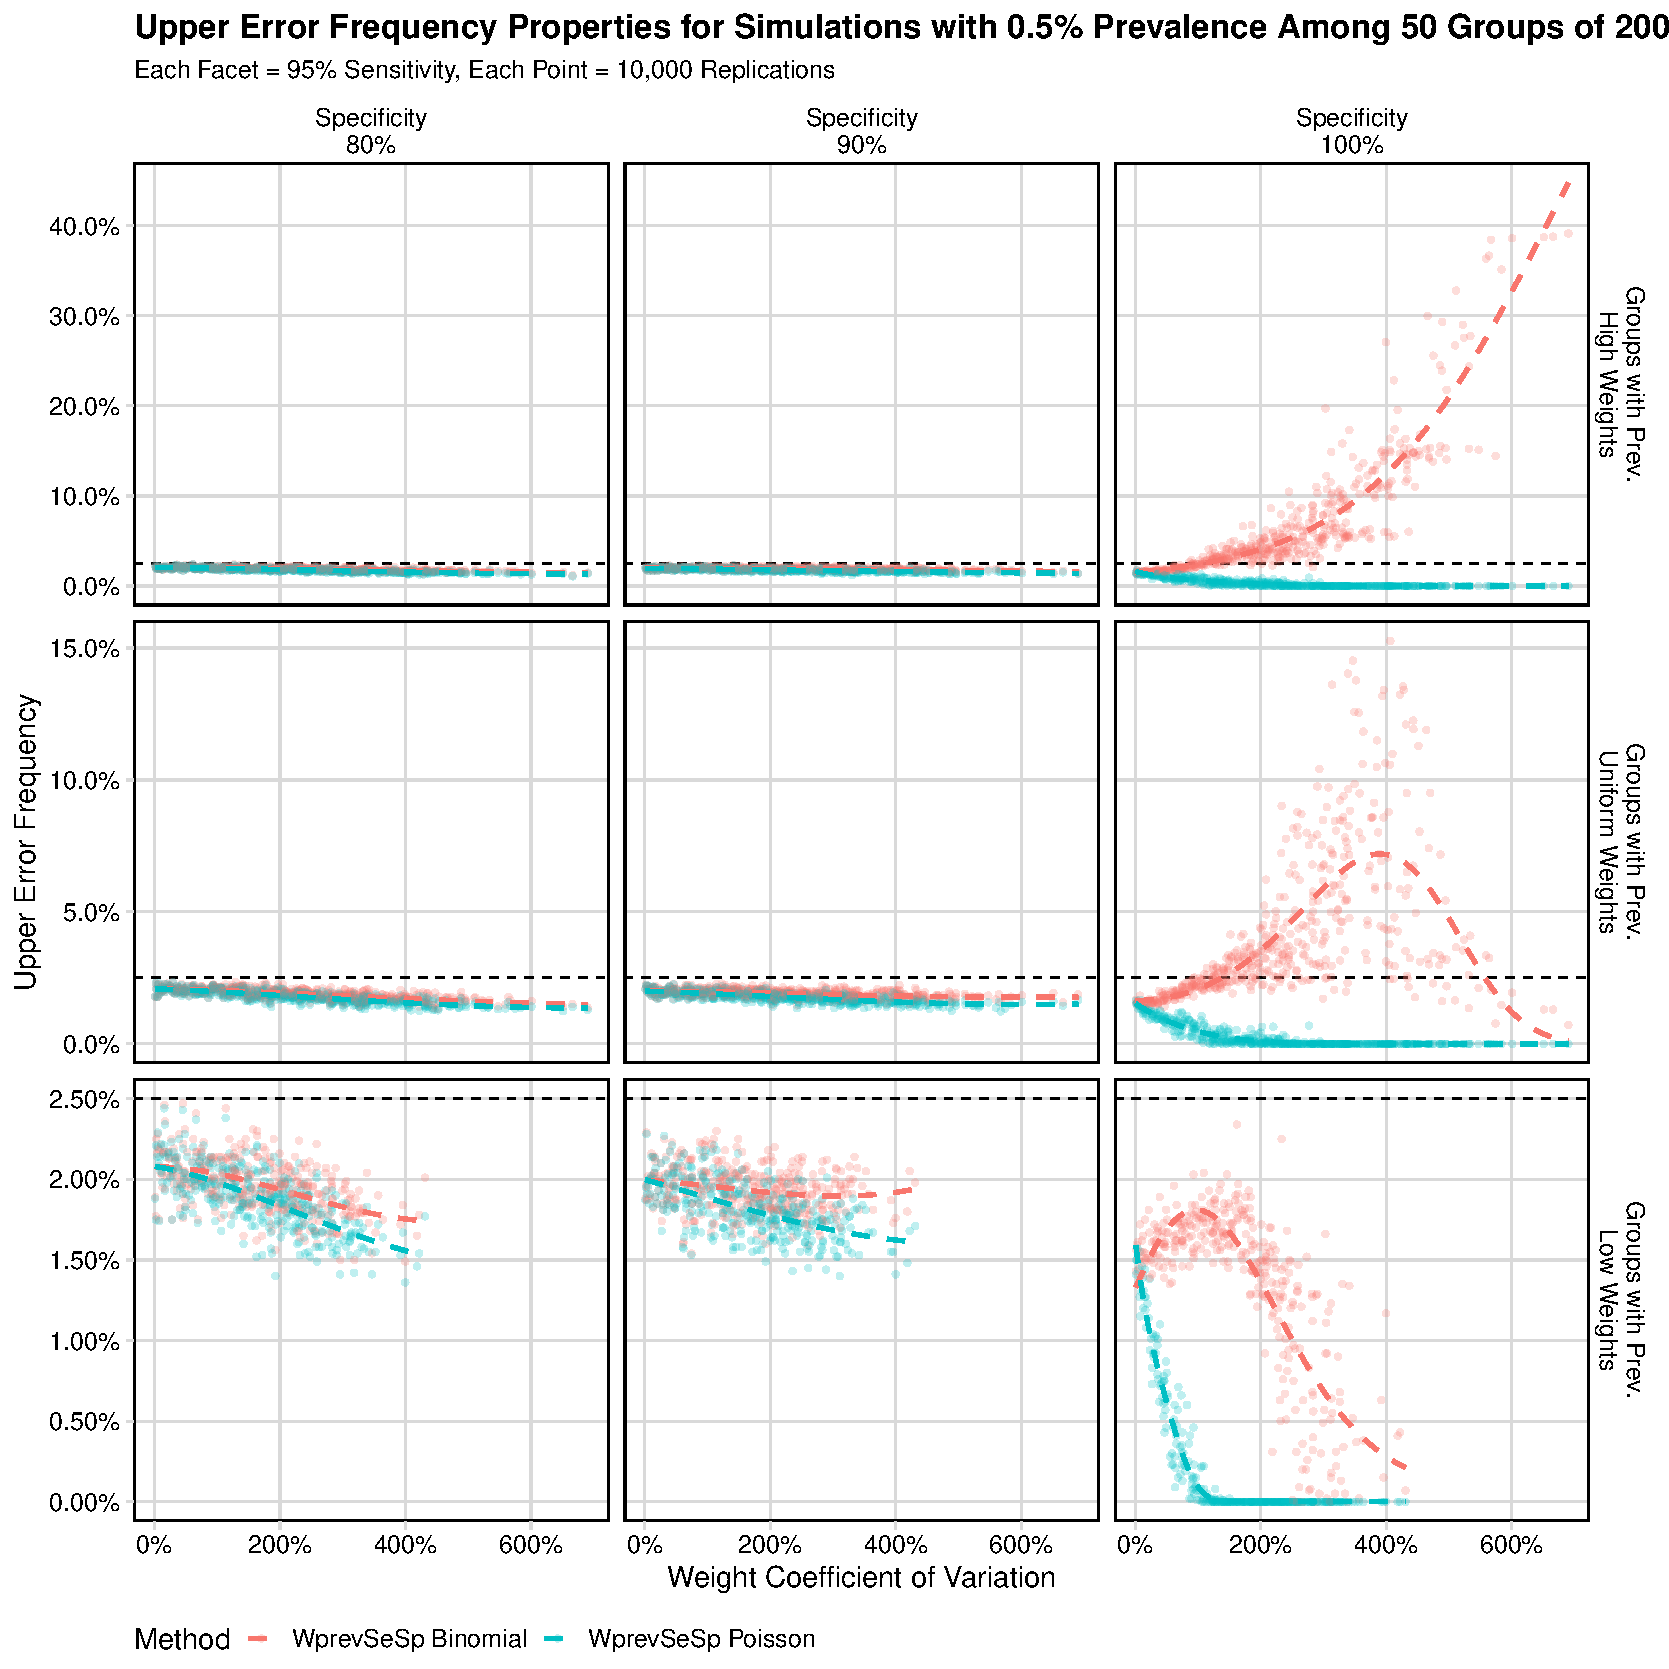
\includegraphics[width=0.8\textwidth]{imperfect_upper_error_frequency_50_groups_0_005_prev}
\caption{Upper error properties for the confidence interval procedures, WprevSeSp Binomial and WprevSeSp Poisson.
Each point represents 10,000 simulations of datasets from a population with 0.5\% prevalence, where 50 groups of 200 people are sampled.
Each dataset also includes simulated results of tests to evaluate the sensitivity and specificity of the assay performed on 60 and 300 individuals, respectively.
The horizontal dashed line indicates the nominal upper error rate, 2.5\%.
Colored dashed lines are estimates from a logistic regression model using quadratic splines.}
\label{ch_3:fig:imperfect_upper_error_frequency_50_groups_0_005_prev}
\end{figure}

\begin{figure}
\centering
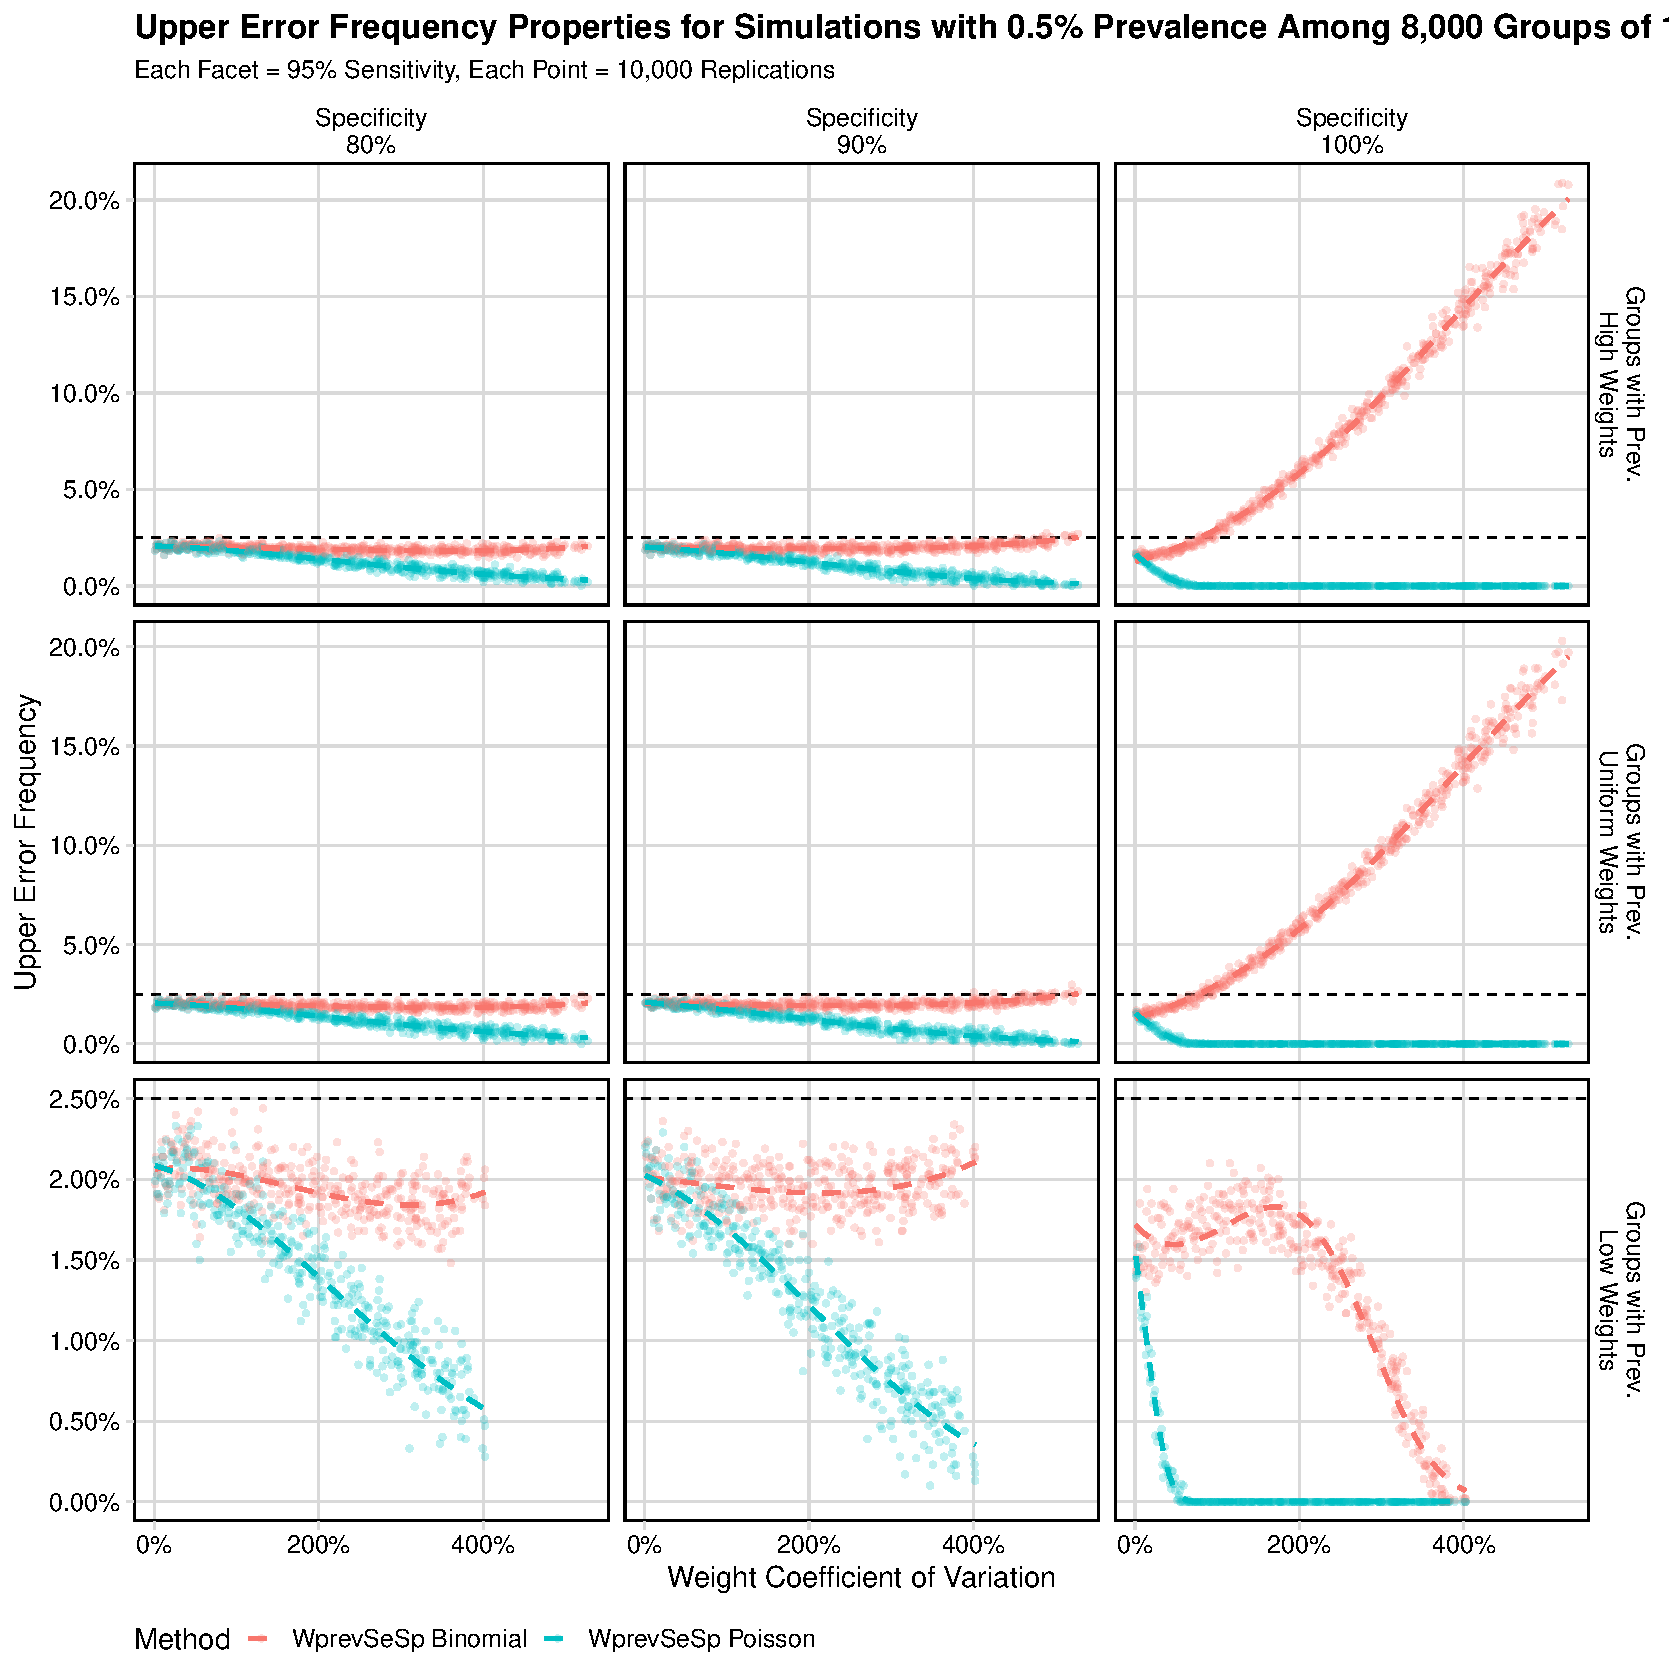
\includegraphics[width=0.8\textwidth]{imperfect_upper_error_frequency_8000_groups_0_005_prev}
\caption{Upper error properties for the confidence interval procedures, WprevSeSp Binomial and WprevSeSp Poisson.
Each point represents 10,000 simulations of datasets from a population with 0.5\% prevalence, where 8000 individuals are sampled.
Each dataset also includes simulated results of tests to evaluate the sensitivity and specificity of the assay performed on 60 and 300 individuals, respectively.
The horizontal dashed line indicates the nominal upper error rate, 2.5\%.
Colored dashed lines are estimates from a logistic regression model using quadratic splines.}
\label{ch_3:fig:imperfect_upper_error_frequency_8000_groups_0_005_prev}
\end{figure}

\begin{figure}
\centering
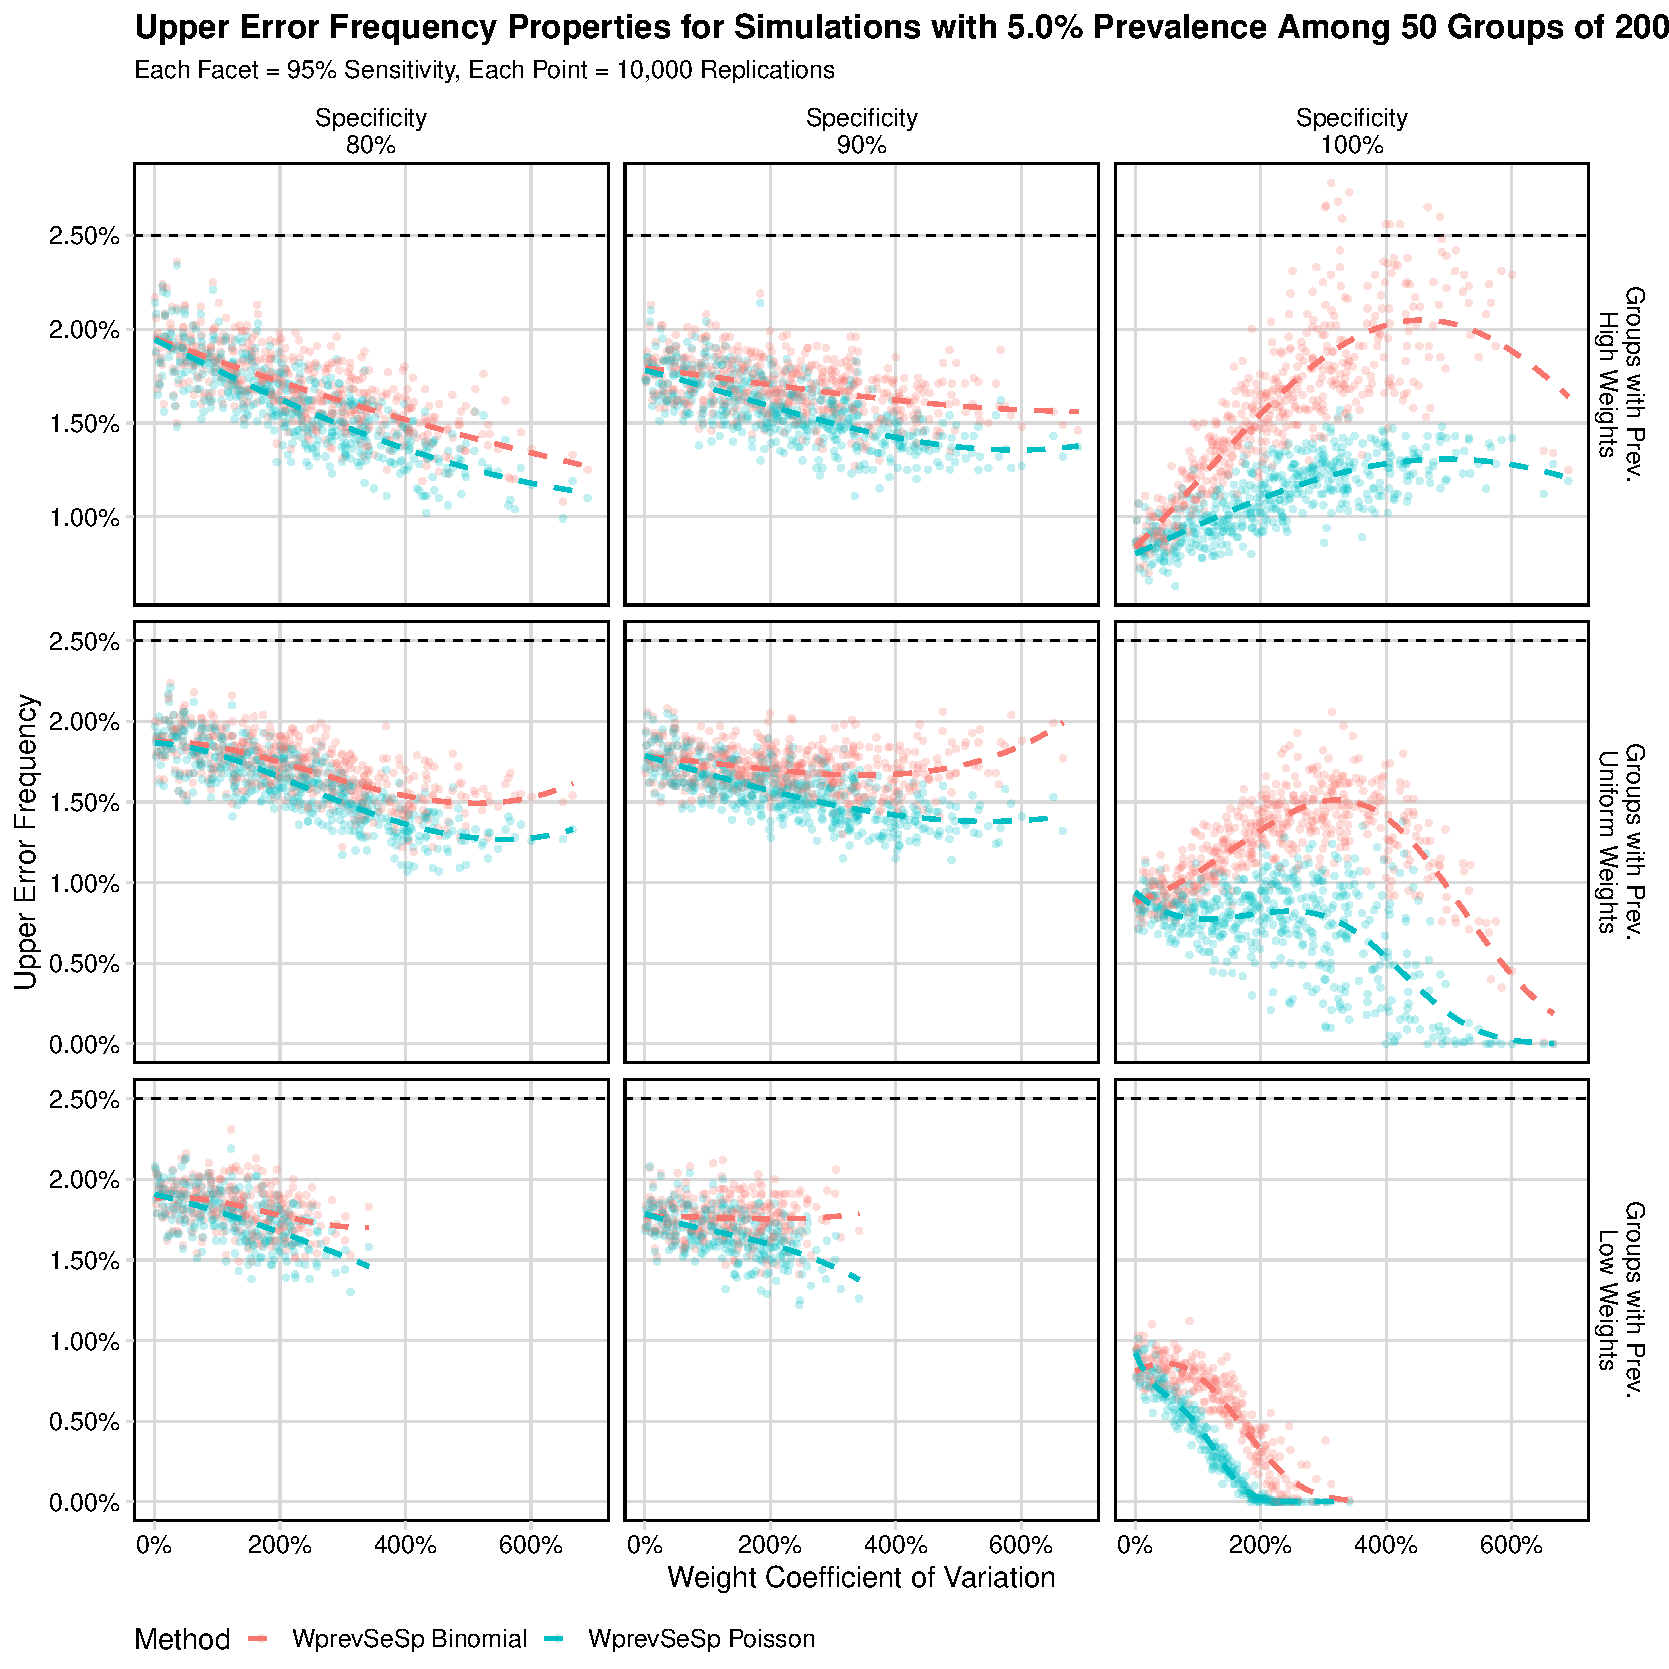
\includegraphics[width=0.8\textwidth]{imperfect_upper_error_frequency_50_groups_0_05_prev}
\caption{Upper error properties for the confidence interval procedures, WprevSeSp Binomial and WprevSeSp Poisson.
Each point represents 10,000 simulations of datasets from a population with 5\% prevalence, where 50 groups of 200 people are sampled.
Each dataset also includes simulated results of tests to evaluate the sensitivity and specificity of the assay performed on 60 and 300 individuals, respectively.
The horizontal dashed line indicates the nominal upper error rate, 2.5\%.
Colored dashed lines are estimates from a logistic regression model using quadratic splines.}
\label{ch_3:fig:imperfect_upper_error_frequency_50_groups_0_05_prev}
\end{figure}

\begin{figure}
\centering
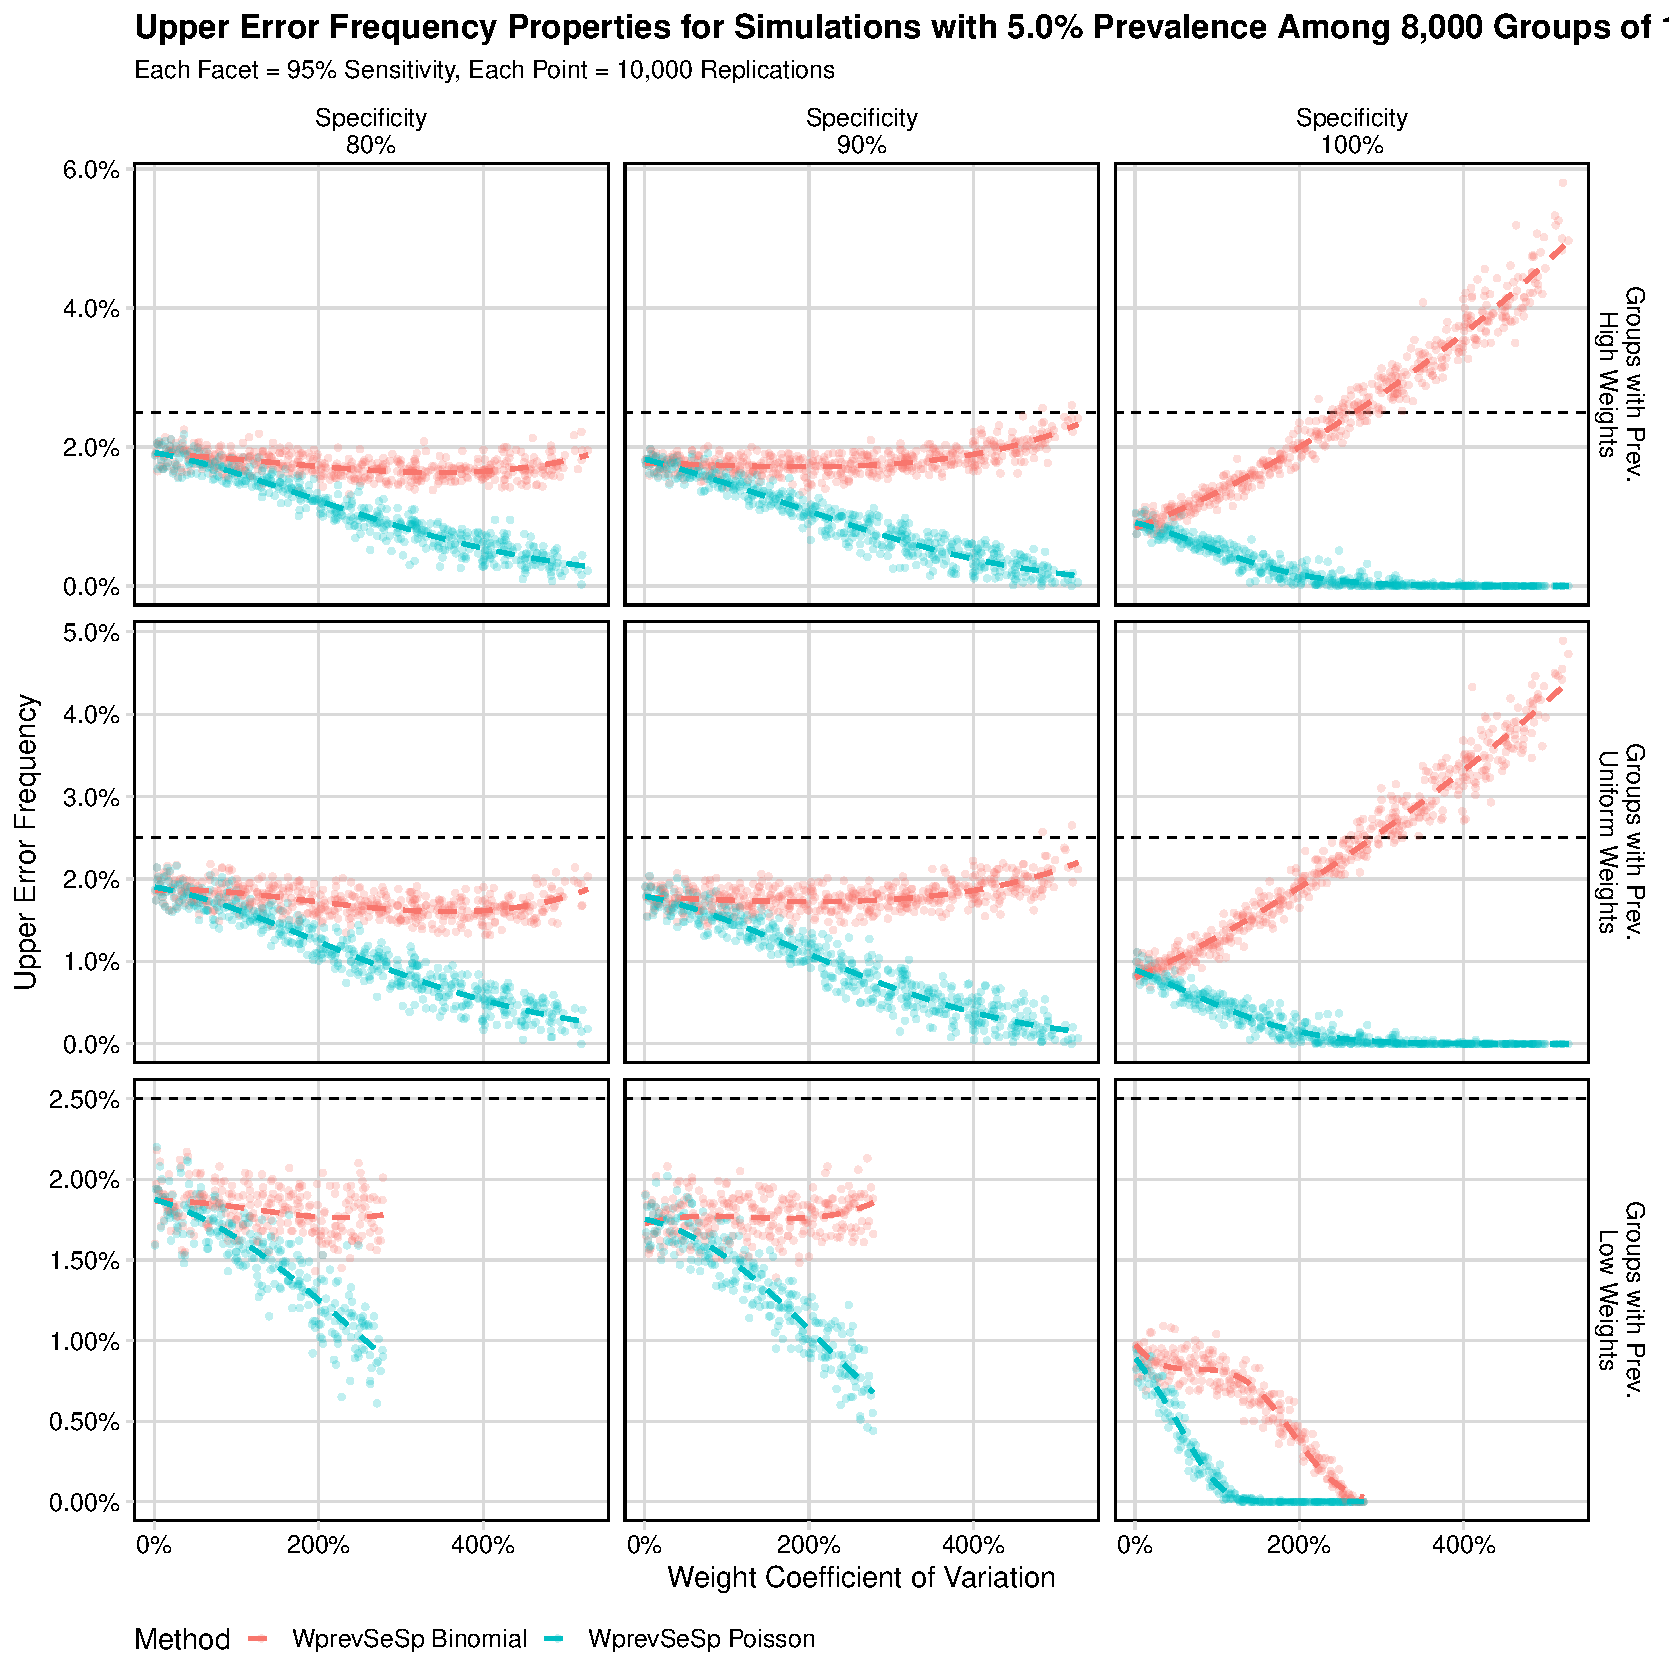
\includegraphics[width=0.8\textwidth]{imperfect_upper_error_frequency_8000_groups_0_05_prev}
\caption{Upper error properties for the confidence interval procedures, WprevSeSp Binomial and WprevSeSp Poisson.
Each point represents 10,000 simulations of datasets from a population with 5\% prevalence, where 8000 individuals are sampled.
Each dataset also includes simulated results of tests to evaluate the sensitivity and specificity of the assay performed on 60 and 300 individuals, respectively.
The horizontal dashed line indicates the nominal upper error rate, 2.5\%.
Colored dashed lines are estimates from a logistic regression model using quadratic splines.}
\label{ch_3:fig:imperfect_upper_error_frequency_8000_groups_0_05_prev}
\end{figure}

\begin{figure}
\centering
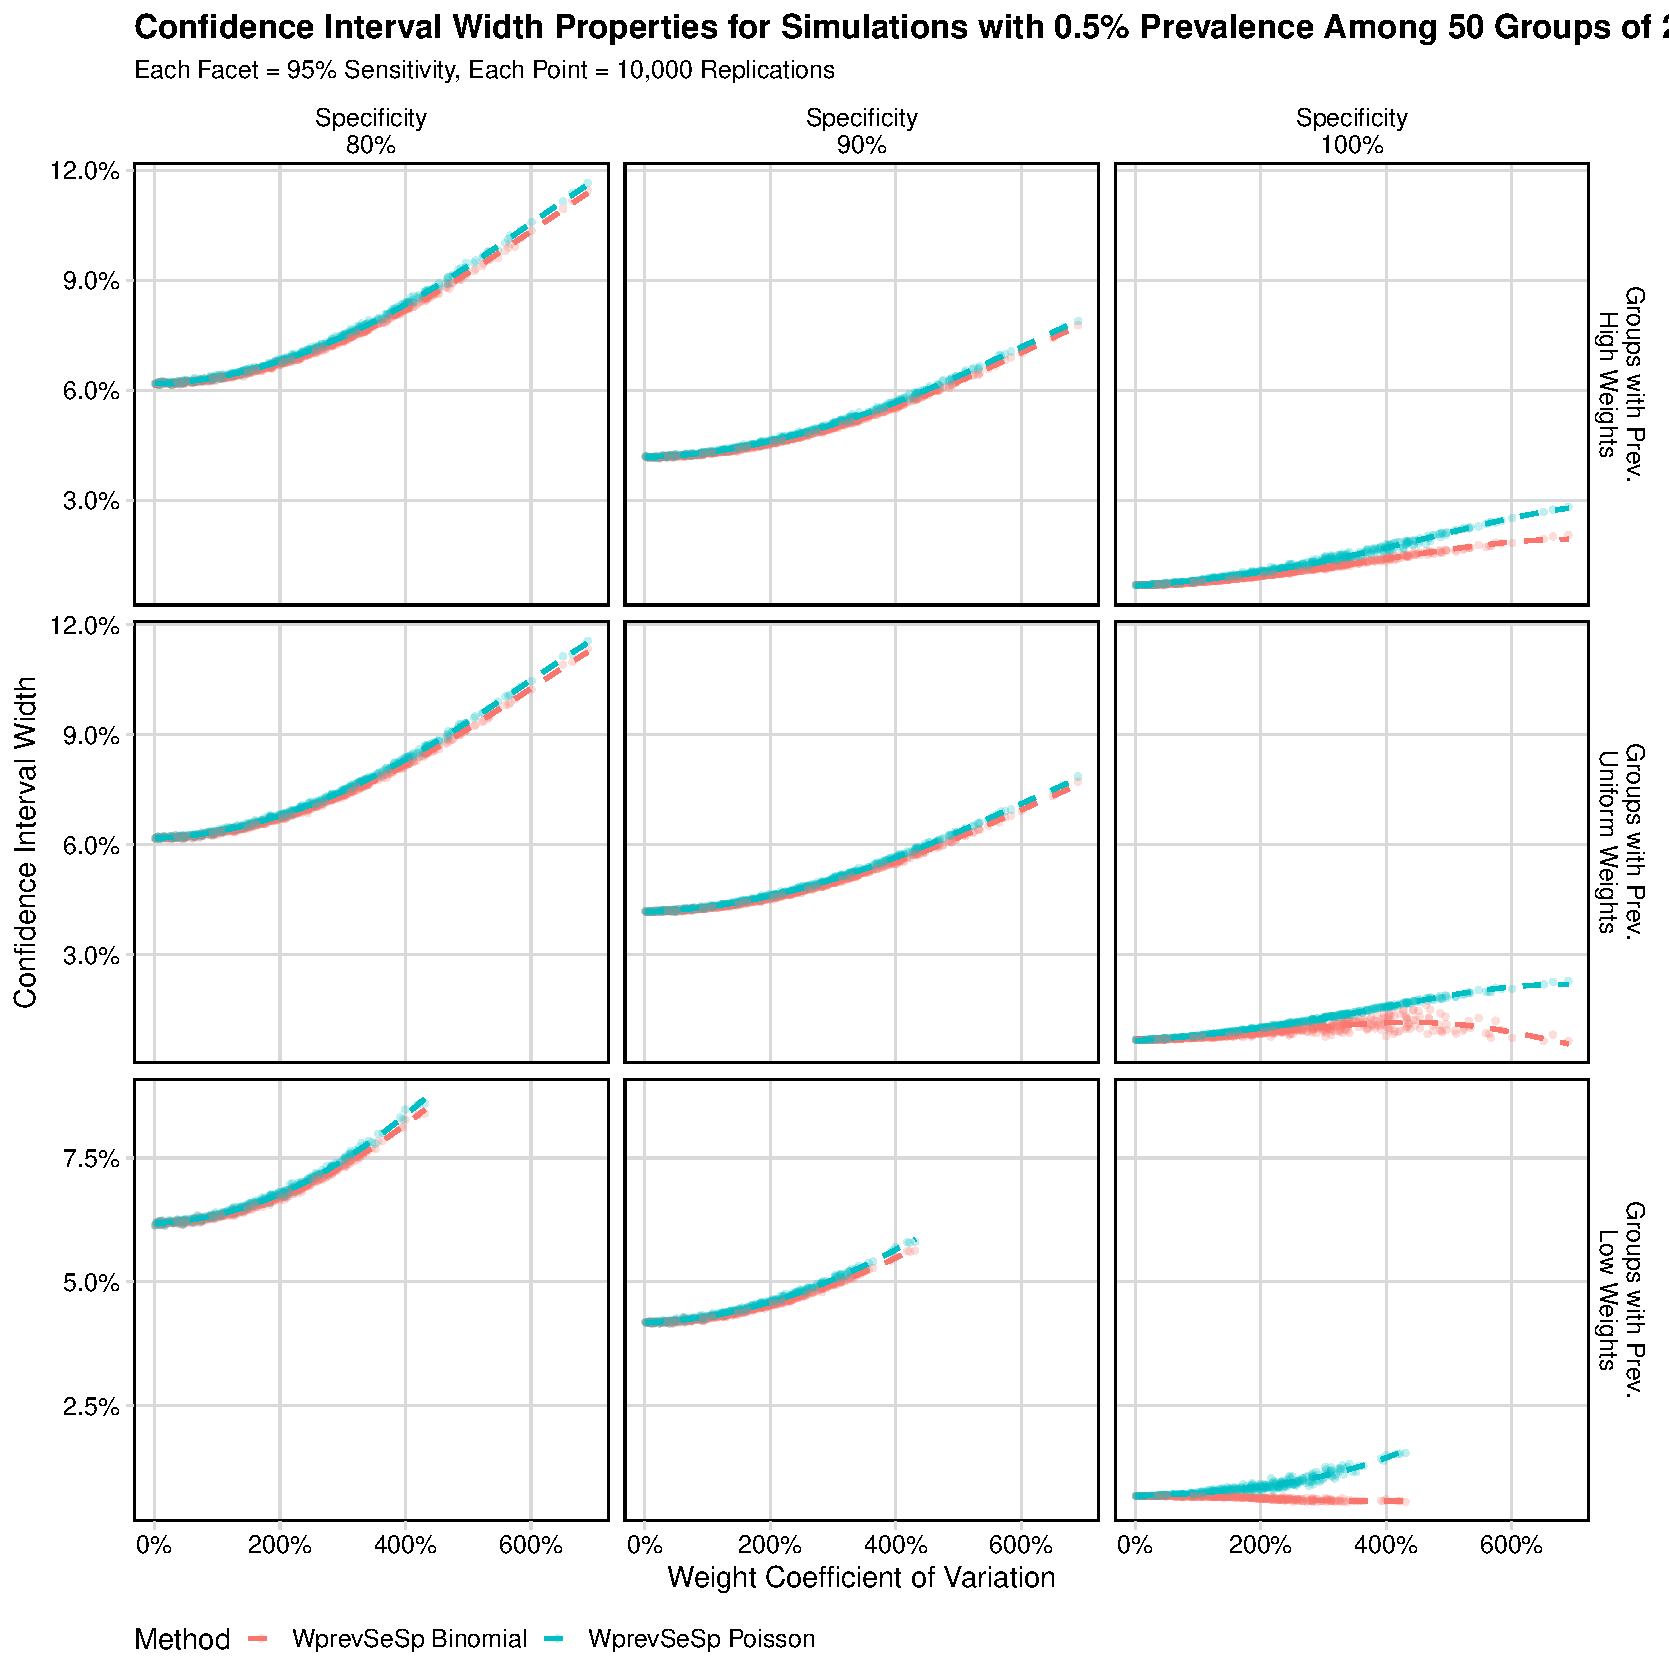
\includegraphics[width=0.8\textwidth]{imperfect_confidence_interval_width_50_groups_0_005_prev}
\caption{Confidence interval width properties for the confidence interval procedures, WprevSeSp Binomial and WprevSeSp Poisson.
Each point represents 10,000 simulations of datasets from a population with 0.5\% prevalence, where 50 groups of 200 people are sampled.
Each dataset also includes simulated results of tests to evaluate the sensitivity and specificity of the assay performed on 60 and 300 individuals, respectively.
Colored dashed lines are estimates from a logistic regression model using quadratic splines.}
\label{ch_3:fig:imperfect_confidence_interval_width_50_groups_0_005_prev}
\end{figure}


\begin{figure}
\centering
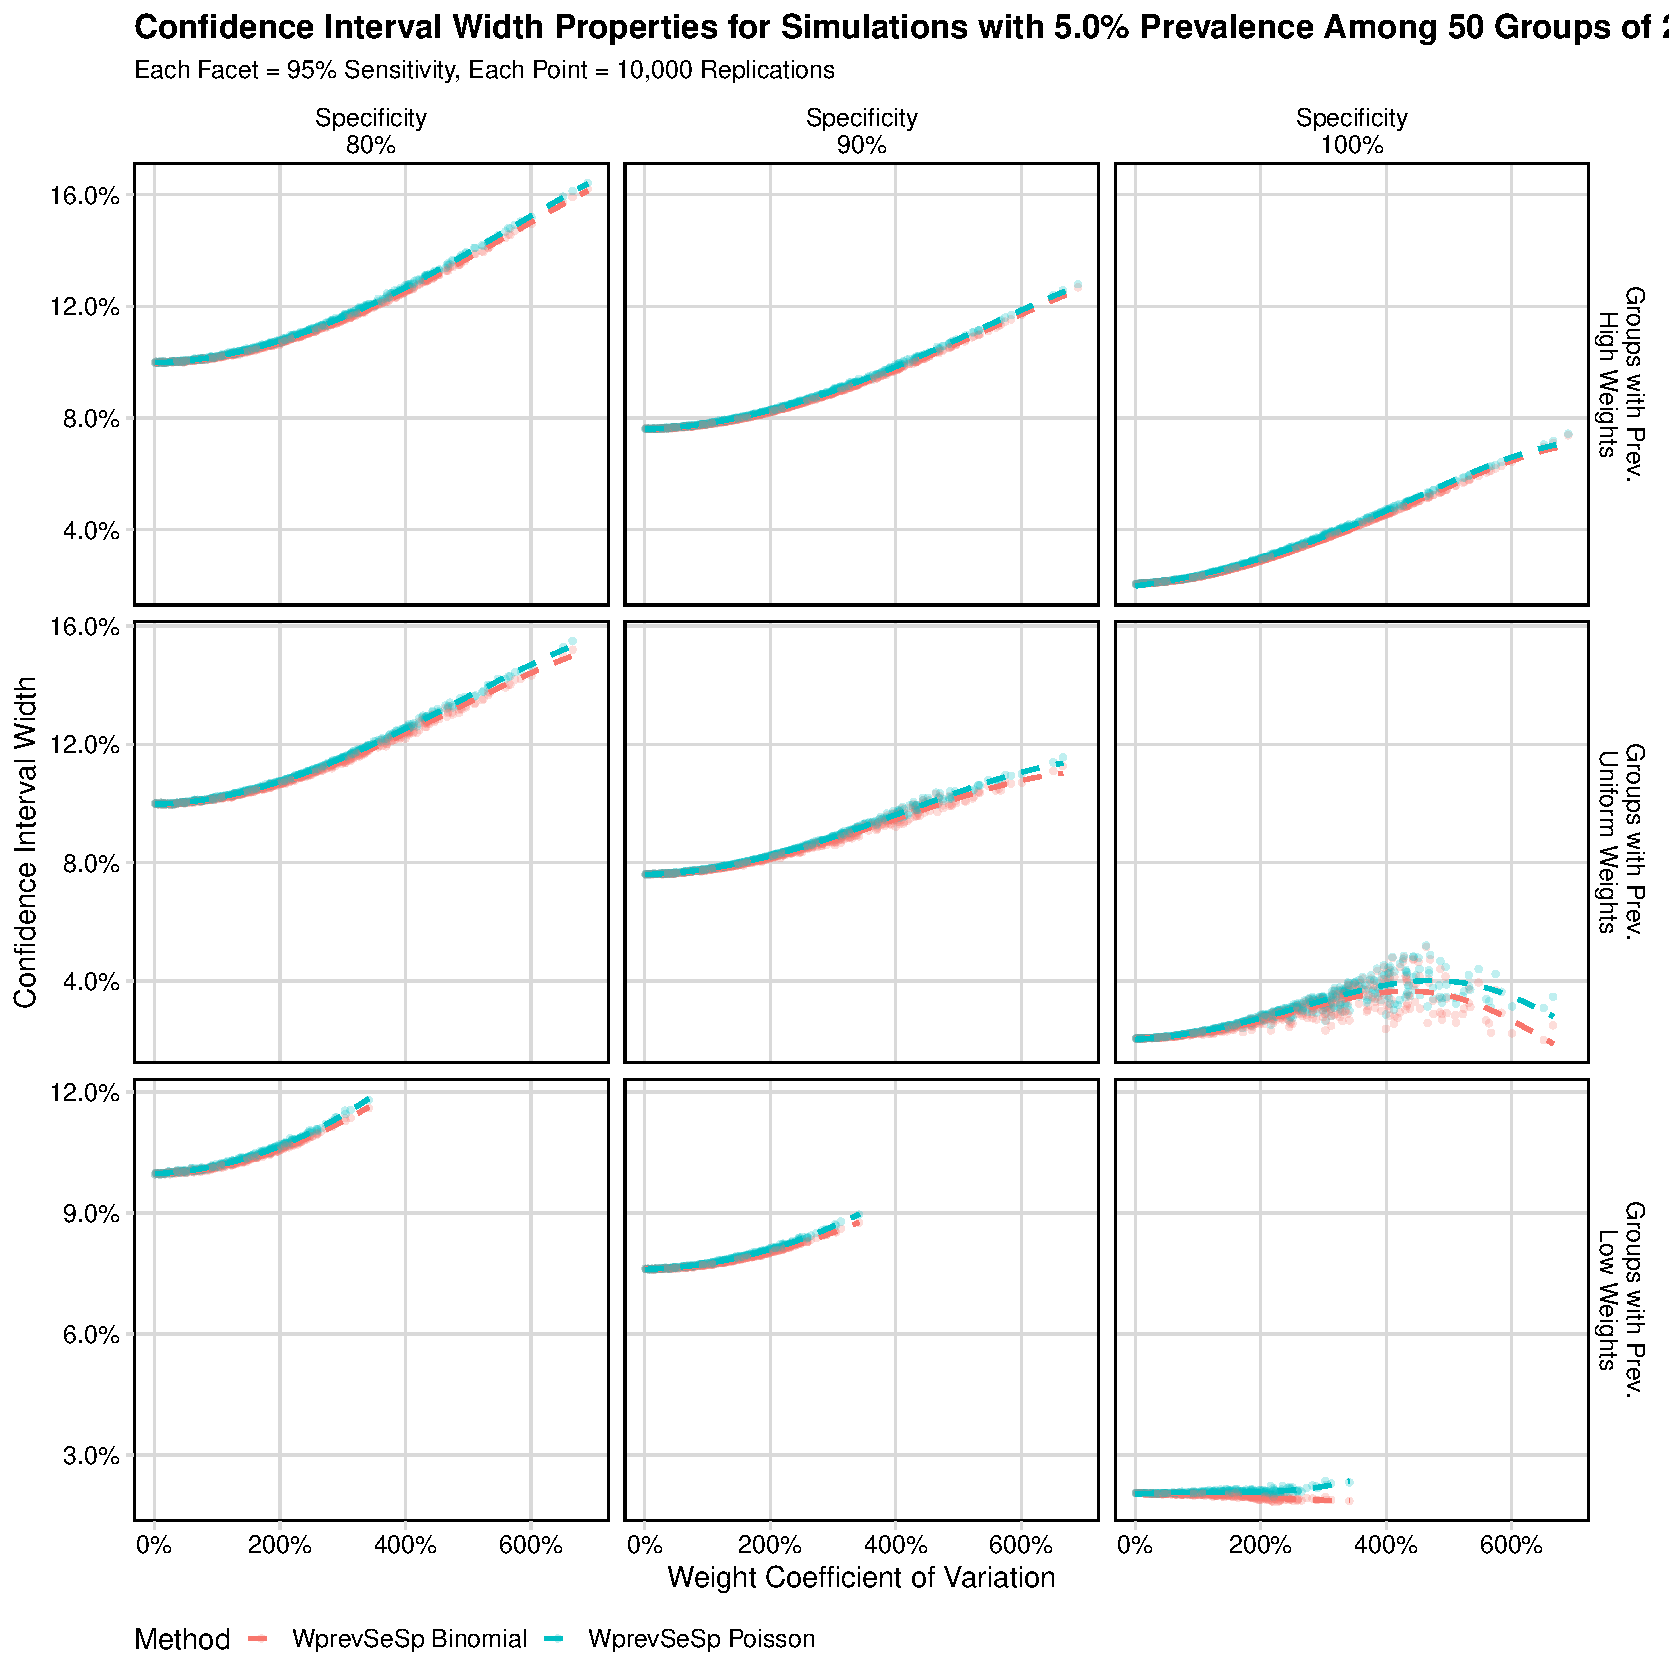
\includegraphics[width=0.8\textwidth]{imperfect_confidence_interval_width_50_groups_0_05_prev}
\caption{Confidence interval width properties for the confidence interval procedures, WprevSeSp Binomial and WprevSeSp Poisson.
Each point represents 10,000 simulations of datasets from a population with 5\% prevalence, where 50 groups of 200 people are sampled.
Each dataset also includes simulated results of tests to evaluate the sensitivity and specificity of the assay performed on 60 and 300 individuals, respectively.
Colored dashed lines are estimates from a logistic regression model using quadratic splines.}
\label{ch_3:fig:imperfect_confidence_interval_width_50_groups_0_05_prev}
\end{figure}


\begin{figure}
\centering
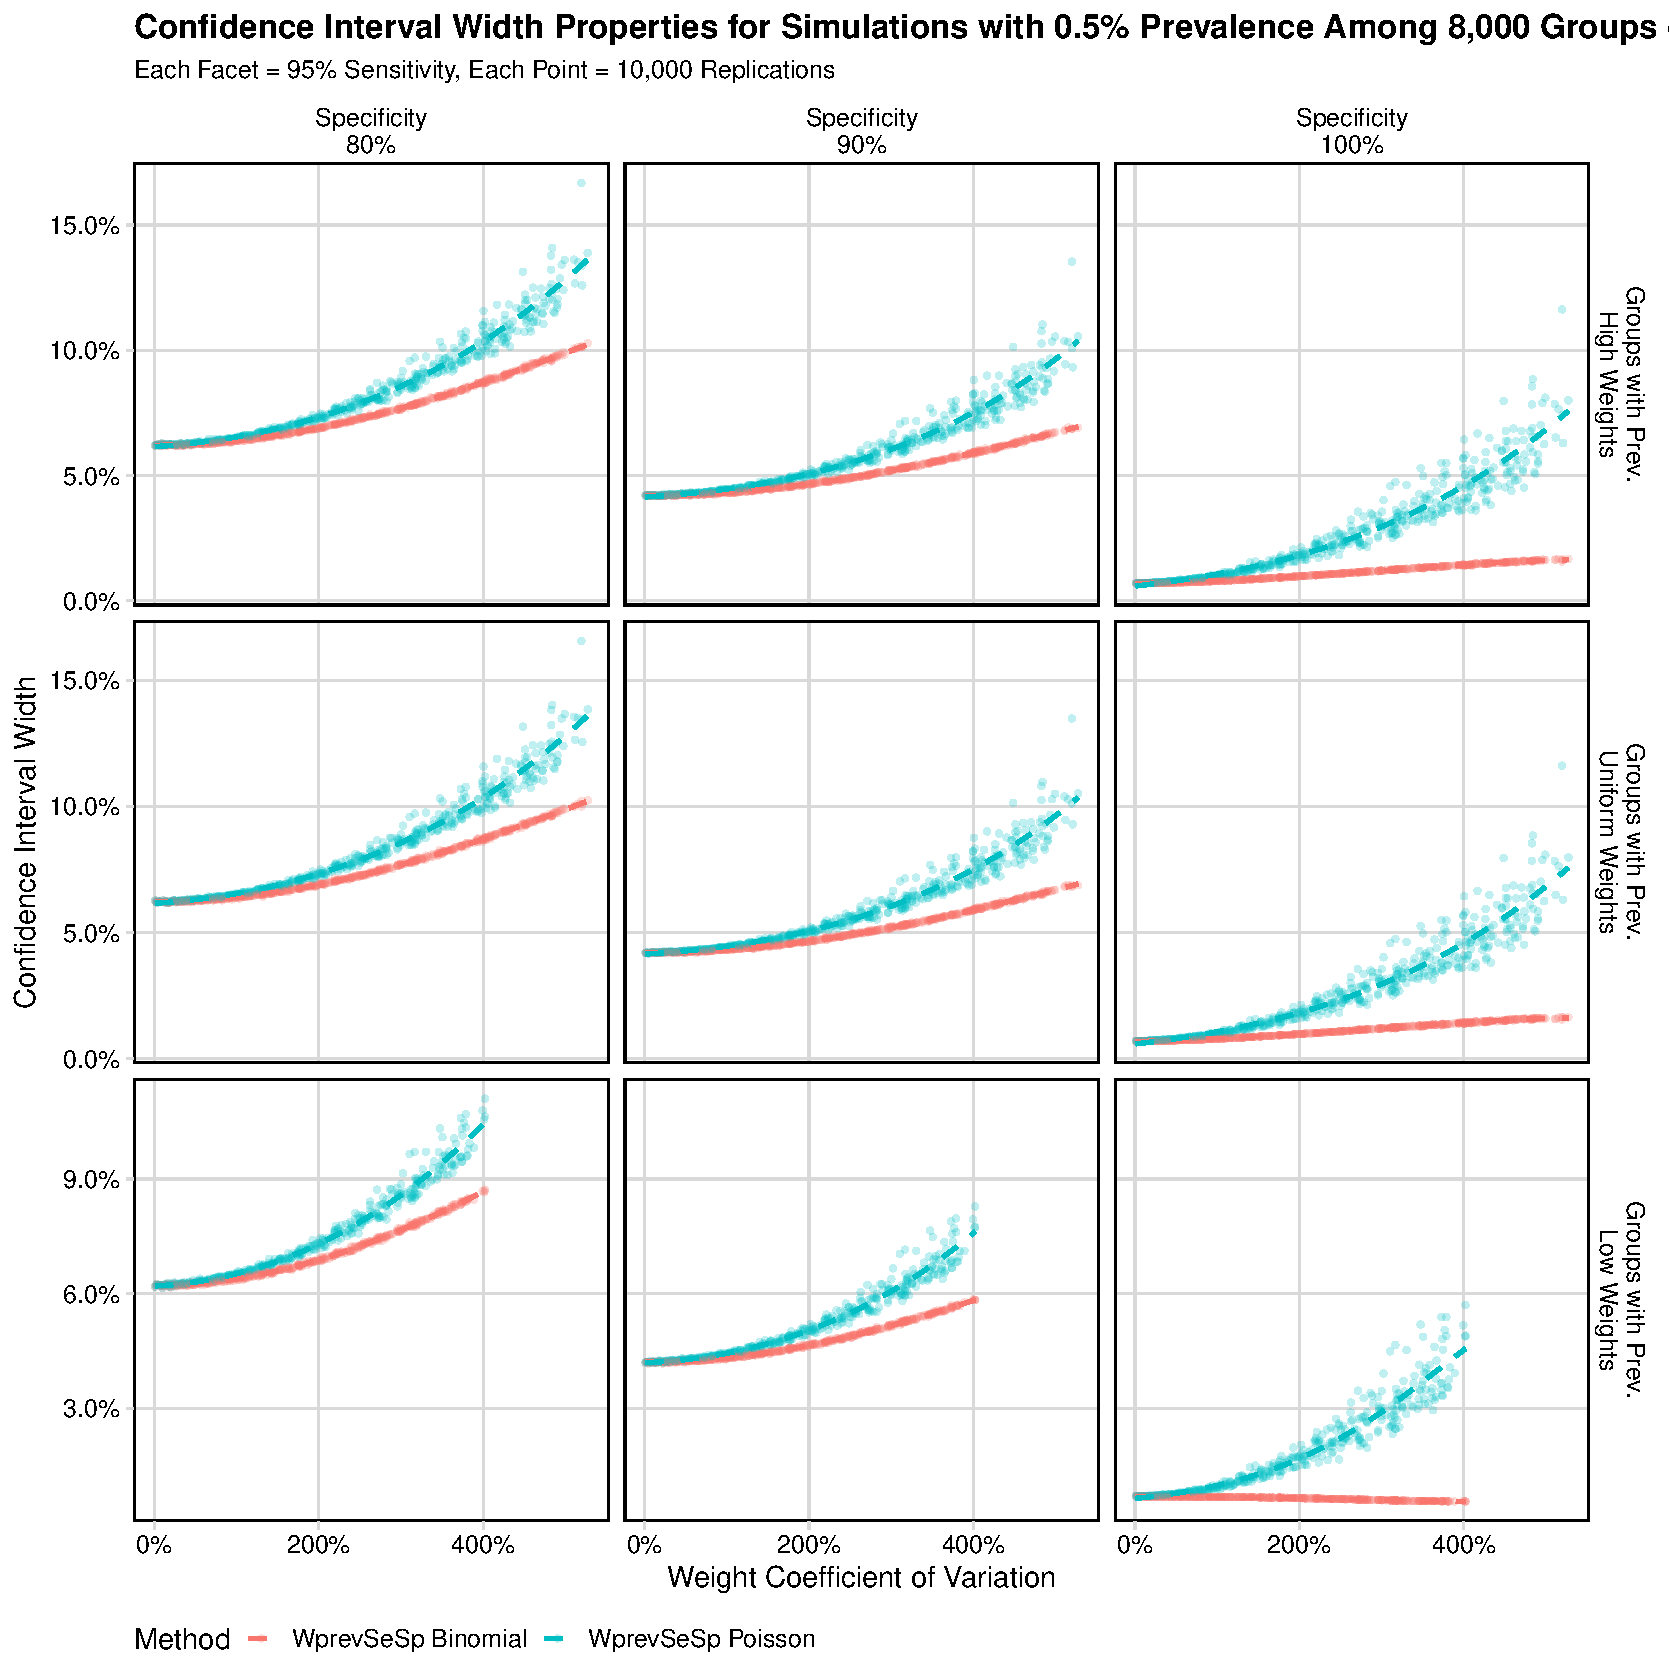
\includegraphics[width=0.8\textwidth]{imperfect_confidence_interval_width_8000_groups_0_005_prev}
\caption{Confidence interval width properties for the confidence interval procedures, WprevSeSp Binomial and WprevSeSp Poisson.
Each point represents 10,000 simulations of datasets from a population with 0.5\% prevalence, where 8000 individuals are sampled.
Each dataset also includes simulated results of tests to evaluate the sensitivity and specificity of the assay performed on 60 and 300 individuals, respectively.
Colored dashed lines are estimates from a logistic regression model using quadratic splines.}
\label{ch_3:fig:imperfect_confidence_interval_width_8000_groups_0_005_prev}
\end{figure}


\begin{figure}
\centering
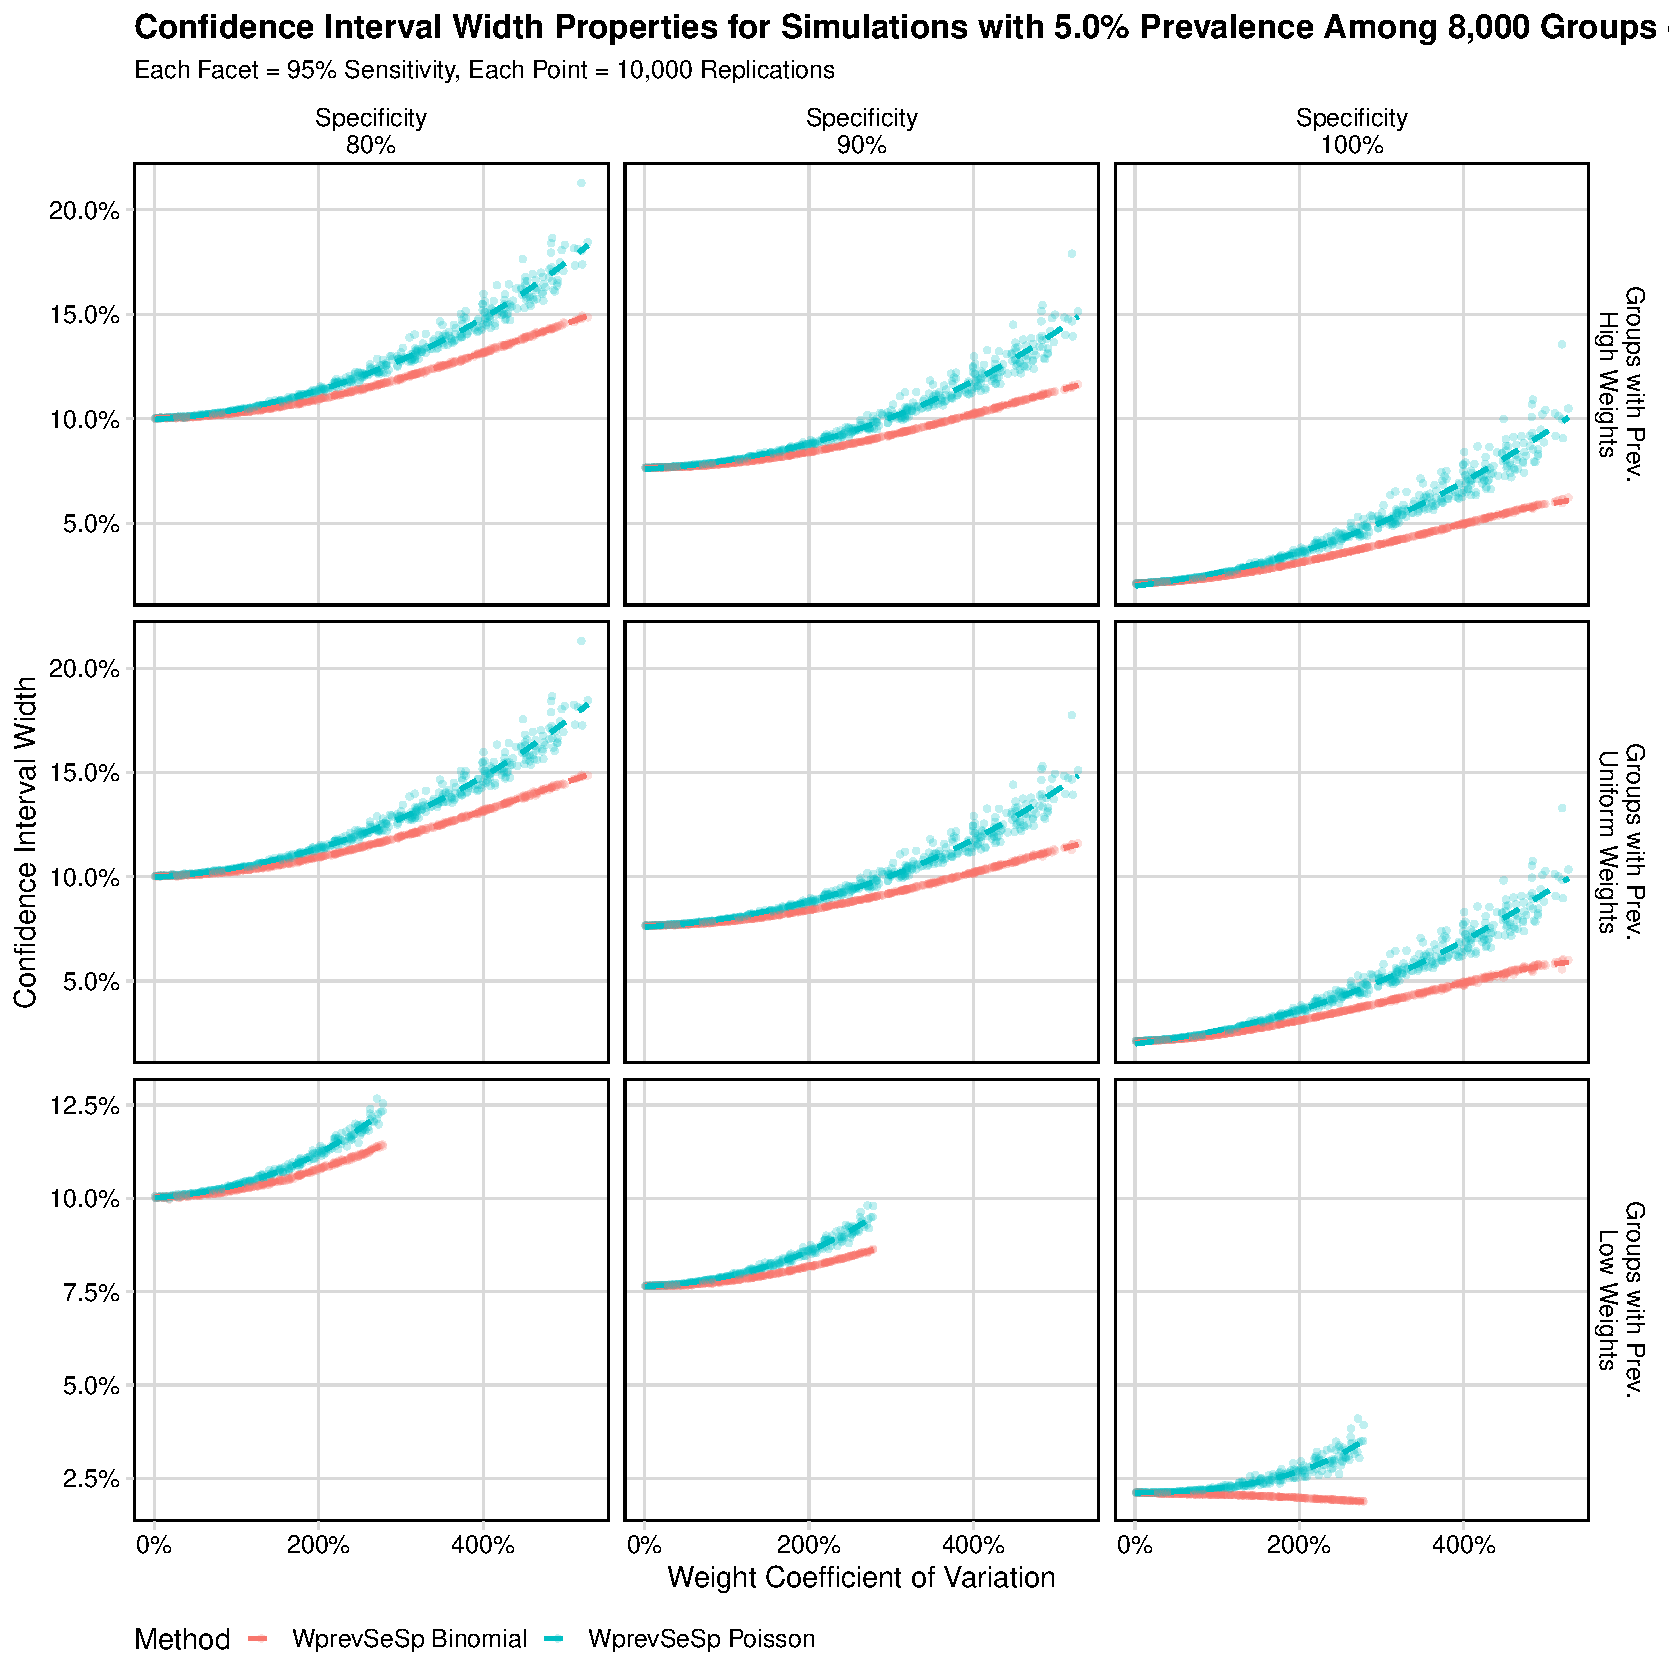
\includegraphics[width=0.8\textwidth]{imperfect_confidence_interval_width_8000_groups_0_05_prev}
\caption{Confidence interval width properties for the confidence interval procedures, WprevSeSp Binomial and WprevSeSp Poisson.
Each point represents 10,000 simulations of datasets from a population with 5\% prevalence, where 8000 individuals are sampled.
Each dataset also includes simulated results of tests to evaluate the sensitivity and specificity of the assay performed on 60 and 300 individuals, respectively.
Colored dashed lines are estimates from a logistic regression model using quadratic splines.}
\label{ch_3:fig:imperfect_confidence_interval_width_8000_groups_0_05_prev}
\end{figure}

\addtocontents{toc}{\protect\setcounter{tocdepth}{2}}